\section{Steps 1 and 2: A priori \texorpdfstring{$G$}{G}-loop estimates}\label{Sec:Steps12}


The remainder of the paper is devoted to proving \Cref{lem:main_ind}, according to the six steps outlined following its statement.
Most of the arguments extend directly to the block Anderson model, with technical differences arising in Step 1 and in the treatment of the light-weight term \smash{$\mathcal{E}^{\Gc,(2)}$} (defined in \eqref{def_EwtG}) when controlling the 2-$G$-loops---specifically, in the proofs of \Cref{lem:LWterm,lem: EWGn2_N} below. %and \Cref{lem:LWterm_EXP} (Step 6). 
We will describe the necessary modifications to adapt the argument to the block Anderson model in \Cref{sec:ext-to-BA}.


\subsection{Proof of Step 1} 

Our proof depends crucially on the following lemma, which provides estimates on the resolvent entries via bounds on 2-$G$-loops. Specifically, \eqref{GiiGEX} and \eqref{GavLGEX} establish bounds on both the entrywise and averaged differences between $G$ and $M$ in the $\max$-norm sense, while \eqref{GijGEX} provides a finer estimate on the off-diagonal resolvent entries, which allows us to derive the decay of the resolvent entries from the decay of the 2-$G$-loops.  


\begin{lemma}\label{lem_GbEXP}
Consider the setting of the random band matrix model. For any $t\in [0,t_0]$, define the event 
\begin{equation}\label{def_asGMc}
    \Omega(t, \e_0) := \big\{\|G_t - M\|_{\max} \leq W^{-\e_0} \big\}
\end{equation}
for a small constant $\e_0>0$. Then, the following \emph{entrywise local law} holds for any constants $\tau,D>0$: 
\begin{equation}
 \P\Big(\mathbf 1(\Omega(t, \e_0))\cdot \|G_{t}-M\|_{\max}^2 \le W^\tau \max_{a,b\in \Zn} \cL^{(2)}_{t,(-,+),(a,b)} \Big)\ge 1-W^{-D} \, .\label{GiiGEX}
\end{equation}
Furthermore, we have the following pointwise decay estimate of $G_t$ for all $a,b\in \Zn$:
\begin{align}\label{GijGEX}
\mathbf 1(\Omega(t, \e_0))\cdot \max_{\substack{x\in [a], y \in [b], x\ne y}} |(G_t)_{xy}|^{2}  \prec & \sum_{\substack{|a'-a|\le 1,|b'-b|\le 1,\\ \bsig\in \{(+,-),(-,+)\}}}  \cL^{(2)}_{t,\bsig,(a',b')}+ W^{-d}\mathbf 1_{|a-b|\le 1}  \, .
\end{align}
Finally, suppose the following estimates hold for a deterministic control parameter $W^{-d/2}\le \Psi_t \le W^{-\e_0}$:\footnote{This parameter $\Psi_t$ should be distinguished from the matrix $\Psi$ appearing in the block Anderson Hamiltonian \eqref{eq:H_blocka}.}
\be\label{initialGT2} 
\|G_{t} - M \|_{\max}\prec W^{-\e_0} ,\quad \max_{a,b\in \Zn} \cL^{(2)}_{t,(-,+),(a,b)} \prec \Psi_t^2 \, . 
\ee
Then, we have the \emph{averaged local law}: 
\begin{align}
\max_{a} \left|\tr\p{\left(G_{t}-M\right)E_{a}} \right| &\prec \Psi_t^2  \, . \label{GavLGEX}
\end{align}
\end{lemma}
\begin{proof}
These estimates have been proven as Lemma 4.1 in \cite{YY_25} for 1D random band matrices. However, their proofs are dimension-independent and use standard arguments based on resolvent identities and large deviation estimates as in \cite{erdHos2012rigidity,erdos2013delocalization}.     
\end{proof}

Step 1 of the proof of \Cref{lem:main_ind} is similar to that in \cite[Section 5.1]{YY_25}, where the core is to establish the following continuity estimate for the $G$-loops. 

\begin{lemma}\label{lem_ConArg}
Fix any \(\e \le s \leq t \leq 1\) for a constant \(\e > 0\). In the flow setting given by \Cref{def_flow} and \Cref{zztE}, assume that the following bound holds at time \(s\) for any fixed $n\in \N$: 
\begin{equation}\label{eq:loopbound_s}
    \max_{\bsig, {\ba}} \abs{{\cal L}^{(n)}_{s, \bsig, {\ba}}} \prec(W^{-d}B_{s,0})^{n-1}.
\end{equation}
% Next, we let $\Omega$ denote the following event:
% \begin{equation}\label{usuayzoo}
%     \Omega := \left\{\|G_{t_2}\|_{\max} \leq 2\right\}.
% \end{equation}
Then, on the event \(\Omega_t= \left\{\|G_{t}\|_{\max} \leq C_0\right\}\) for a constant $C_0>0$, the following estimate holds for any fixed \(n \in \N\) with $n\ge 2$:
\begin{equation}\label{res_lo_bo_eta}
    {\bf 1}(\Omega_t) \cdot \max_{\bsig, {\ba}} \big|{\cal L}^{(n)}_{t, \bsig, {\ba}} \big|\prec \left(
    (W^{-d}B_{s,0})\cdot\frac{\eta_{s}}{\eta_{t}}\right)^{n-1}
    \le  \left(
    (W^{-d}B_{t,0})\cdot\frac{\eta_{s}}{\eta_{t}}\right)^{n-1}.
\end{equation}
\end{lemma} 
\begin{proof}%[Proof of Lemma \ref{lem_ConArg}]%\label{sec:Inh_LE}
The proof of this lemma is exactly the same as that for Lemma 5.1 in \cite{YY_25}, except for some minor changes in notation. Hence, we omit the details.\end{proof}

%Now, combining \Cref{lem_GbEXP,lem_ConArg}, we can readily conclude the proof of Step 1 with a standard continuity argument. 

%\begin{proof}[\bf Step 1: Proof of \eqref{lRB1} and \eqref{Gtmwc}]
With \Cref{lem_GbEXP,lem_ConArg}, Step 1 of the proof of \Cref{lem:main_ind} for the random band matrix model (i.e., the proof of \eqref{lRB1} and \eqref{Gtmwc}) is the same as that in \cite[Section 5.1]{YY_25}. Hence, we omit the details. 
%\end{proof}


\subsection{Dynamics of  \texorpdfstring{$(\cal L-\cal K)$-loops}{L-K}}\label{subsec:DyLK}

We begin by presenting some representations of the $G$-loop dynamics, formulated using the loop hierarchy \eqref{eq:mainStoflow}, Duhamel's principle, and certain evolution kernels, which we introduce below. This dynamics has already been derived for random band matrices in \cite{YY_25} and for the block Anderson model in \cite{RBSO1D}, and will be the basis for Step 2 and subsequent steps of the proof of \Cref{lem:main_ind}. 
For any fixed $n\in \N$, combining the loop hierarchy \eqref{eq:mainStoflow} and the convolution tree equation \eqref{pro_dyncalK}, we obtain the following SDE for the $(\cL-\cK)$-loops as shown in equation (5.12) of \cite{YY_25}: 
\begin{align}\label{eq_L-Keee}
    \dd(\mathcal{L} - \mathcal{K})^{(n)}_{t, \bsig, \ba} = &\left[\cK^{(2)} \sim (\mathcal{L} - \mathcal{K})\right]^{(n)}_{t, \bsig, \ba} \, \dd t+\sum_{\lenk=3}^n \left[\cK^{(\lenk)}\sim (\mathcal{L} - \mathcal{K})\right]^{(n)}_{t, \bsig, \ba}\, \dd t \nonumber\\
    &+ \mathcal{E}^{(\cL-\cK)\times (\cL-\cK),(n)}_{t, \bsig, \ba}\dd t+\mathcal{E}^{\Gc,(n)}_{t, \bsig, \ba}\dd t + \dd\mathcal{E}^{M,(n)}_{t, \bsig, \ba} .
\end{align} 
% \begin{align}\label{eq_L-K-1}
%        \dd(\mathcal{L} - \mathcal{K})^{(n)}_{t, \bsig, \ba} 
%     =&~ W^d \sum_{1 \leq k < l \leq n} \sum_{a,b} 
%    (\mathcal{L} - \mathcal{K})^{(n+k-l+1)}_{t, \cutL^{(a)}_{k, l}\left(\bsig,\, \ba\right)} S^{(\sB)}_{ab}
%    \mathcal{K}^{(l-k+1)}_{t,\cutR^{(b)}_{k,l}\left(\bsig ,\ba\right)}\, \dd t \nonumber\\
%     +&~ W^d \sum_{1 \leq k < l \leq n} \sum_{a,b} \mathcal{K}^{(n+k-l+1)}_{t, \cutL^{(a)}_{k, \,l}\left(\bsig,\ba\right)} 
%    S^{(\sB)}_{ab}\left(\cL-\cK\right)^{(l-k+1)}_{t,\cutR^{(b)}_{k, l}\left(\bsig,\ba\right)} \, \dd t \nonumber\\
%    +&~ \mathcal{E}^{(\cL-\cK)\times (\cL-\cK),(n)}_{t, \bsig, \ba}\dd t+\mathcal{E}^{\Gc,(n)}_{t, \bsig, \ba}
%     \dd t + 
%     \dd\mathcal{E}^{M,(n)}_{t, \bsig, \ba}  ,
% \end{align}
Here, every \smash{$\cK^{(\lenk)}$}, $2\le \lenk\le n$, is regarded as a linear operator acting on the $(\cL-\cK)$-loops, defined as:
\begin{align}\label{DefKsimLK}
&\left[\cK^{(\lenk)}\sim (\mathcal{L} - \mathcal{K})\right]_{t, \bsig, \ba}^{(n)}:= W^d \sum_{1\le k < l \leq n : l-k=\lenk-1} \sum_{a,b} 
   (\mathcal{L} - \mathcal{K})^{(n-\lenk+2)}_{t, \cutL^{(a)}_{k, l}\left(\bsig,\, \ba\right)} 
S^{(\sB)}_{ab}\mathcal{K}^{(\lenk)}_{t,\cutR^{(b)}_{k,l}\left(\bsig ,\ba\right)} \nonumber\\
&\quad +  W^d \sum_{1 \leq k < l \leq n:l-k=n-\lenk+1} \sum_{a,b} \mathcal{K}^{(\lenk)}_{t, \cutL^{(a)}_{k, \,l}\left(\bsig,\ba\right)} S^{(\sB)}_{ab}
   \left(\cL-\cK\right)^{(n-\lenk+2)}_{t,\cutR^{(b)}_{k, l}\left(\bsig,\ba\right)} ,
\end{align}
$\mathcal{E}^{\Gc}$ and $\dd\mathcal{E}^{M}$ are defined in \eqref{def_EwtG} and \eqref{def_Edif}, respectively, and the term $\mathcal{E}^{(\cL-\cK)\times (\cL-\cK)}$ is defined by 
\begin{equation}\label{def_ELKLK}
\mathcal{E}^{(\cL-\cK)\times (\cL-\cK),(n)}_{t, \bsig, \ba} :=
    W^d \sum_{1 \leq k < l \leq n} \sum_{a,b} 
   (\mathcal{L} - \mathcal{K})^{(n+k-l+1)}_{t, \cutL^{(a)}_{k, l}\left(\bsig,\, \ba\right)} 
  S^{(\sB)}_{ab} (\cL-\mathcal{K})^{(l-k+1)}_{t,\cutR^{(b)}_{k,l}\left(\bsig ,\ba\right)}\,  .
\end{equation}
In \eqref{eq_L-Keee}, the superscript ``$(n)$'' indicates the length of the $(\cL-\cK)$-loop on the LHS of the equation, and we will sometimes omit it from our notations when the value of $n$ is clear from the context. 


We now rewrite \eqref{eq_L-Keee} into an integral equation using Duhamel's principle. First, we introduce the evolution kernel associated with this integral equation.


\begin{definition}[Evolution kernel]\label{DefTHUST}
For each $t\in [0,1)$, fixed $n\ge 2$ and $\bsig=(\sigma_1,\ldots,\sig_n)\in \{+,-\}^n$, we define the linear operator ${\varTheta}^{(n)}_{t, \bsig}$ acting on $n$-dimensional tensors ${\cal A}: (\Zn)^{n}\to \mathbb C$ as follows (recall \eqref{eq:Msig}):
\begin{align}\label{def:op_thn}
    \left({\varTheta}^{(n)}_{t, \bsig} \circ \mathcal{A}\right)_{\ba} & = \sum_{i=1}^n \sum_{b_i\in\Zn} \left(\frac{M^{(\sig_i,\sig_{i+1})}S^{(\sB)}}{1 - t M^{(\sig_i,\sig_{i+1})}S^{(\sB)}}\right)_{a_ib_i}  \mathcal{A}_{\ba^{(i)}(b_i)},
\end{align} 
where $\ba=(a_1,\ldots, a_n)\in (\Zn)^n$, \(\ba^{(i)}(b_i):= (a_1, \ldots, a_{i-1}, b_i, a_{i+1}, \ldots, a_n),\) and we adopt the cyclic convention that $\sigma_{n+1}=\sig_1$.  
The evolution kernel corresponding to ${\varTheta}^{(n)}_{t, \bsig}$ is given by
    \begin{align}\label{def_Ustz}
        \left(\mathcal{U}_{s, t, \bsig}^{(n)} \circ \mathcal{A}\right)_{\ba} = \sum_{\mathbf{b} = (b_1, \ldots, b_{n})} \prod_{i=1}^n \left(\frac{1 - s \cdot M^{(\sig_i,\sig_{i+1})} S^{(\sB)} }{1 - t \cdot M^{(\sig_i,\sig_{i+1})} S^{(\sB)}}\right)_{a_i b_i} \cdot \mathcal{A}_{\mathbf{b}} . 
    \end{align}
% Define the linear map ${\varTheta}_{t, \bsig}$ via the following action on a tensor ${\cal A}: \mathbb Z^n_L\to \mathbb C$: 
% \begin{align}\label{def:op_thn}
%     \left({{\varTheta}}_{t, \bsig} \circ \mathcal{A}\right)_{{\ba}} & = \sum_{i=1}^n \sum_{b_i} \left(\frac{m_i m_{i+1}  }{1 - t m_i m_{i+1} S^{(B)}}\right)_{a_i b_i} \cdot \mathcal{A}_{{\ba}^{(i)}},\quad m_i=m(\sigma_i) \nonumber \\
%     \quad {\ba}^{(i)}&  = (a_1, \ldots, a_{i-1}, b_i, a_{i+1}, \ldots, a_n).
% \end{align}  
% We also define the semigroup operator $\mathcal{U}_{s,t,\bsig}$ associated to $\Theta_{t,\bsig}$ as follows
%     \begin{align}\label{def_Ustz}
%         \left(\mathcal{U}_{s, t, \bsig} \circ \mathcal{A}\right)_{{\ba}} = \sum_{b_1, \ldots, b_n} \prod_{i=1}^n \left(\frac{1 - s \cdot m_i m_{i+1} S^{(B)}}{1 - t \cdot m_i m_{i+1} S^{(B)}}\right)_{a_i b_i} \cdot \mathcal{A}_{\textbf{b}}, \quad \textbf{b} = (b_1, \ldots, b_n), \quad m_i=m(\sigma_i)
%     \end{align}
\end{definition}


By the definition of the 2-$\cK$-loop in \eqref{Kn2sol}, we observe that the first term on the RHS of \eqref{eq_L-Keee} can be rewritten as ${\varTheta}^{(n)}_{t, \bsig} \circ (\mathcal{L} - \mathcal{K})^{(n)}_{t,\bsig}$. With this fact and using Duhamel's principle, we obtain the following lemma.


\begin{lemma}[Integrated loop hierarchy, Lemma 5.3 of \cite{YY_25}] \label{Sol_CalL}
First, \eqref{eq_L-Keee} is equivalent to the integral equation: for any stopping time $\tau\ge s$ with respect to the matrix Brownian motion $\{H_t\}$,
\begin{align}\label{int_K-L_ST}
({\cal L}-{\cal K})^{(n)}_{\tau,\bsig,{\ba}}&=({\cal L}-{\cal K})^{(n)}_{s,\bsig,{\ba}}+\int_{s}^{\tau}\p{\varTheta^{(n)}_{u,\bsig}\circ({\cal L}-{\cal K})^{(n)}_{u,\bsig}}_{{\ba}}\dd u+\sum_{l_\mathcal{K}=3}^n \int_s^\tau \Big[\mathcal{K}^{(\lenk)} \sim (\mathcal{L} - \mathcal{K})\Big]^{(n)}_{u, \bsig, {\ba}}\dd u \nonumber\\
&+ \int_s^\tau \mathcal{E}^{(\mathcal{L} - \mathcal{K}) \times (\mathcal{L} - \mathcal{K}),(n)}_{u, \bsig, {\ba}}\dd u + \int_{s}^{\tau}\mathcal{E}^{\Gc,(n)}_{u, \bsig, {\ba}}\dd u + \int_s^\tau \dd \mathcal{E}^{M,(n)}_{u, \bsig, {\ba}} .
\end{align}
%    
%Then we have the (simple version) of loop hierarchy (\textcolor{blue}{new})  \begin{align}\label{int_K-LcalE_simple}    (\mathcal{L} - \mathcal{K})_{t, \bsig, {\ba}} \;=\; \; &     (\mathcal{L} - \mathcal{K})_{s, \bsig,{\ba}}     \; + \;\sum_{l_\mathcal{K}\ge 2} \int_{s}^t    \Big[\mathcal{K} \sim (\mathcal{L} - \mathcal{K})\Big]^{l_\mathcal{K}}_{u, \bsig, {\ba}} du \nonumber \\   &+ \int_{s}^t   \mathcal{E}^{((\mathcal{L} - \mathcal{K}) \times (\mathcal{L} - \mathcal{K}))}_{u, \bsig, {\ba}} du \;+\; \int_{s}^t  \mathcal{E}^{(\widetilde{G})}_{u, \bsig, {\ba}} du + \int_{s}^t  \mathcal{E}^{(M)}_{u, \bsig, {\ba}}  
%\end{align}
Second, applying Duhamel's principle to \eqref{eq_L-Keee}, we obtain the following \emph{integrated loop hierarchy}:
\begin{align}\label{int_K-LcalE}
   & (\mathcal{L} - \mathcal{K})^{(n)}_{t, \bsig, \ba}  =
    \left(\mathcal{U}^{(n)}_{s, t, \bsig} \circ (\mathcal{L} - \mathcal{K})^{(n)}_{s, \bsig}\right)_{\ba} + \sum_{l_\mathcal{K} =3}^n \int_{s}^t \left(\mathcal{U}^{(n)}_{u, t, \bsig} \circ \Big[\cK^{(\lenk)}\sim (\mathcal{L} - \mathcal{K})\Big]^{(n)}_{u, \bsig}\right)_{\ba} \dd u \nonumber \\
    &+ \int_{s}^t \left(\mathcal{U}^{(n)}_{u, t, \bsig} \circ \mathcal{E}^{(\cL-\cK)\times(\cL-\cK),(n)}_{u, \bsig}\right)_{\ba} \dd u  + \int_{s}^t \left(\mathcal{U}^{(n)}_{u, t, \bsig} \circ \mathcal E^{\Gc,(n)}_{u, \bsig}\right)_{\ba} \dd u + \int_{s}^t \left(\mathcal{U}^{(n)}_{u, t, \bsig} \circ \dd \mathcal E^{M,(n)}_{u, \bsig}\right)_{\ba} .
\end{align}
% \begin{align}\label{int_K-LcalE}
%     (\mathcal{L} - \mathcal{K})_{t, \bsig, {\ba}} \;=\; \; &
%     \left(\mathcal{U}_{s, t, \bsig} \circ (\mathcal{L} - \mathcal{K})_{s, \bsig}\right)_{{\ba}} \nonumber \\
%     &+ \sum_{l_\mathcal{K} > 2} \int_{s}^t \left(\mathcal{U}_{u, t, \bsig} \circ \Big[\mathcal{K} \sim (\mathcal{L} - \mathcal{K})\Big]^{l_\mathcal{K}}_{u, \bsig}\right)_{{\ba}} du \nonumber \\
%     &+ \int_{s}^t \left(\mathcal{U}_{u, t, \bsig} \circ \mathcal{E}^{((\mathcal{L} - \mathcal{K}) \times (\mathcal{L} - \mathcal{K}))}_{u, \bsig}\right)_{{\ba}} du  \nonumber \\
%     &+ \int_{s}^t \left(\mathcal{U}_{u, t, \bsig} \circ \mathcal{E}^{(\widetilde{G})}_{u, \bsig}\right)_{{\ba}} du + \int_{s}^t \left(\mathcal{U}_{u, t, \bsig} \circ \mathcal{E}^{(M)}_{u, \bsig}\right)_{{\ba}}  
% \end{align}
% \begin{align}\label{int_K-L_ST}
%    (\mathcal{L} - \mathcal{K})_{\tau , \bsig, {\ba}} \;=\; \; &
%     \left(\mathcal{U}_{s, \tau, \bsig} \circ (\mathcal{L} - \mathcal{K})_{s, \bsig}\right)_{{\ba}}  \nonumber \\
%     &+ \sum_{l_\mathcal{K} > 2} \int_{s}^\tau \left(\mathcal{U}_{u, \tau, \bsig} \circ \Big[\mathcal{K} \sim (\mathcal{L} - \mathcal{K})\Big]^{l_\mathcal{K}}_{u, \bsig}\right)_{{\ba}} du  \nonumber \\
%     &+ \int_{s}^\tau \left(\mathcal{U}_{u, \tau, \bsig} \circ \mathcal{E}^{((\mathcal{L} - \mathcal{K}) \times (\mathcal{L} - \mathcal{K}))}_{u, \bsig}\right)_{{\ba}} du  \nonumber \\
%     &+ \int_{s}^\tau \left(\mathcal{U}_{u, \tau, \bsig} \circ \mathcal{E}^{(\widetilde{G})}_{u, \bsig}\right)_{{\ba}} du + \int_{s}^\tau \left(\mathcal{U}_{u, \tau, \bsig} \circ \mathcal{E}^{(M)}_{u, \bsig}\right)_{{\ba}}.
% \end{align}
\end{lemma}


Before returning to the proof of \Cref{lem:main_ind}, we introduce the following notation, which controls the quadratic variation of the martingale term in \eqref{def_Edif}. More precisely, $\dd\cal E^{M,(n)}$ is a sum over the $n$ edges of the loop at which the loop is cut, and the tensor defined below keeps only the terms with the same cut on both sides. Hence, by the Cauchy--Schwarz inequality over the $n$ cuts, the quadratic variation of any linear combination $\sum_{\ba}\varphi_{\ba}\,\dd\cal E^{M,(n)}_{u,\bsig,\ba}$ is bounded by $n\sum_{\ba,\ba'}\varphi_{\ba}\overline{\varphi_{\ba'}}\,(\cal E\otimes\cal E)^{M,(n)}_{u,\bsig,\ba,\ba'}\,\dd u$; in general, the two are not equal because of the cross terms between different cuts. The factor $n$ is absorbed into the constant $C_{n,p}$ in \Cref{lem:DIfREP} below.

 
\begin{definition}[Quadratic variation loop]\label{def:CALE} 
For $t\in [0,1]$ and $\bsig=(\sigma_1,\ldots,\sig_n)\in \{+,-\}^n$, we introduce the $(2n)$-dimensional \emph{quadratic variation tensor} for any \(\ba=(a_1,\ldots, a_n) \) and \(\ba'=(a_1',\ldots, a_n')\):
 %  \begin{align*}
 % \left( \cal E \otimes \cal E  \right)^{M,(n)}_{t, \bsig, \ba, \ba'} \; := \; &
 % \sum_{k=1}^n \left( \cal E \otimes \cal E \right)^{M,(n;k)}_{t,  \bsig, \ba, \ba'},\quad %\forall \ba=(a_1,\ldots, a_n) ,\ \ba'=(a_1',\ldots, a_n'), %\in (\Zn)^n,
 % \end{align*}
 % where each $\left( \cal E \otimes \cal E \right)^{M,(n;k)}_{t,  \bsig, \ba, \ba'}$ is defined as 
\be\label{defEOTE}
 \left( \cal E \otimes \cal E  \right)^{M,(n)}_{t, \bsig, \ba, \ba'} := 
 \sum_{k=1}^n \left( \cal E \otimes \cal E \right)^{M,(n;k)}_{t,  \bsig, \ba, \ba'},\ \ \text{where}\ \ \left( \cal E \otimes \cal E \right)^{M,(n;k)}_{t,  \bsig, \ba, \ba'} :
 =   W^d \sum_{b,b'} S^{(\sB)}_{bb'}{\cal L}^{(2n+2)}_{t, (\bsig\otimes\overline\bsig)^{(k) },(\ba\otimes \ba')^{(k)}(b,b')}.
\ee
Here, ${\cal L}^{(2n+2)}$ denotes a $(2n+2)$-loop obtained by cutting the $k$-th edge of ${\cal L}^{(n)}_{t,\bsig,\ba}$ and then gluing it (with indices $\ba$) with its conjugate loop (with indices $\ba'$) along the newly introduced vertices $b$ and $b'$. Formally:
\begin{align*}
   & {\cal L}^{(2n+2)}_{t, (\bsig\otimes\overline\bsig)^{(k) },(\ba\otimes \ba')^{(k )}(b,b')}:=  \tr \bigg\{ \prod_{i=k}^n \left(G_{t}(\sigma_i) E_{a_i}\right) \cdot \prod_{i=1}^{k-1} \left(G_{t}(\sigma_i) E_{a_i}\right) \cdot G_t(\sigma_k) E_{b} G_t(-\sigma_k) \\
    &\qquad \times \prod_{i={1}}^{k-1} \left(E_{a_{k-i}'} G_{t}(-\sigma_{k-i}) \right)\cdot \prod_{i=k}^{n} \left(E_{a_{n+k-i}'} G_{t}(-\sigma_{n+k-i}) \right) E_{b'}\bigg\} ,
\end{align*}
where the notations $(\ba\otimes \ba')^{(k )}$ and $(\bsig\otimes\overline \bsig)^{(k) }$ (with $\overline\bsig$ denoting $(-\sig_1,\ldots,-\sig_n)$) represent respectively
\begin{align}\label{def_diffakn_k}
 (\ba\otimes \ba')^{(k )}(b,b')&=( a_k,\ldots, a_n, a_1,\ldots , a_{k-1}, b, a'_{k-1},\ldots, a_1', a_n',\ldots, a'_{k},b'),\nonumber \\
  (\bsig\otimes \overline\bsig)^{(k )}&=(  \sigma_k, \ldots, \sigma_n,   \sigma_1,\ldots ,\sigma_{k}, -\sigma_{k}, \ldots, -\sigma_1 ,   -\sigma_n, \ldots, -\sigma_{k }).
\end{align}
%We remark that the symbol ``$\otimes$'' in the above notations is used to emphasize the symmetric structure and does not represent any kind of ``product''. 

% Denote 
%   \begin{align}\label{defEOTE}
%  \left( \mathcal{E}\otimes  \mathcal{E} \right)_{t, \,\bsig, \,{\ba}, \,{\ba}'} \; := \; &
%  \sum_{k=1}^n\left( \mathcal{E}\otimes  \mathcal{E} \right)^{(k)}_{t, \,\bsig, \,{\ba}, \,{\ba}'}
%  \nonumber \\
%  \left( \mathcal{E}\otimes  \mathcal{E} \right)^{(k)}_{t, \,\bsig, \,{\ba}, \,{\ba}'} :
% \; = \; & W^{d} \sum_{b,b'} S^{(B)}_{b,b'}{\cal L}_{t, \bsig^{(k ) },{\ba}^{(k )}},\quad \bsig^{(k ) }\in \{+,-\}^{2n+2}, 
% \end{align}
% where ${\cal L}_{t, \bsig^{(k ) },{\ba}^{(k )}}$ is obtained by cutting the $k$-th edge of ${\cal L}_{t,\bsig,{\ba}}$ and then attaching itself (with indices ${\ba}$) to its complex conjugate loop (with indices ${\ba}'$) into a bigger loop that is labeled by indices $b$ and $b'$, so that
% %where ${\ba}^{(k )}(m)$ is the $m$-th component of ${\ba}^{(k )}$. More precisely
% \begin{align}\label{def_diffakn_k}
%    & {\ba}^{(k )}=( a_k,a_{k+1},\cdots a_n, a_1,\cdots a_{k-1}, b', a'_{k-1}\cdots a_1', a_n'\cdots a'_{k},b)
%     \nonumber \\
%   &  \bsig^{(k )}=( \, \sigma_k, \, \sigma_{k+1},\cdots \sigma_n,  \, \sigma_1,\cdots \sigma_{k}, \,  \overline\sigma_{k},  \cdots \overline\sigma_1 , \,  \overline\sigma_n \cdots \overline\sigma_{k })
% \end{align}
%The symbol $\otimes$ is used to emphasize the symmetric structure of $\mathcal{E} \otimes \mathcal{E}$; it is not a tensor product.  


\end{definition}

 


Under the above notations, applying the Burkholder-Davis-Gundy inequality, we obtain the following lemma that provides high-moment bounds on the martingale term. %is an immediate consequence of the Burkholder-Davis-Gundy inequality.  We now estimate the martingale term in \eqref{int_K-L_ST} via Lemma 5.5 in \cite{YY_25}, which we record below.

\begin{lemma}[Lemma 5.5 of \cite{YY_25}]\label{lem:DIfREP}
Let $\tau$ be a stopping time with respect to the matrix Brownian motion $\{H_t\}$. Then, for any fixed $p\in \N$, there exists a constant $C_{n,p}$ such that
\begin{align}\label{aaswtghh}
   \E \left [    \int_{s}^\tau \dd  \mathcal{E}^{M,(n)}_{u, \bsig, {{\ba}}}  \right ]^{2p} 
   &\le C_{n,p}  
   \E \left(\int_{s}^\tau 
   \left( 
   \left( \mathcal{E} \otimes  \mathcal{E} \right)
  ^{M,(n)}_{u, \bsig, \ba,\ba}  
   \right)\dd u 
   \right)^{p},\\
   \label{alu9_STime}
   \E \left [    \int_{s}^t\left(\mathcal{U}^{(n)}_{u, t, \bsig} \circ \dd\cal E^{M,(n)}_{u, \bsig}\right)_{\ba} \right ]^{2p} 
   &\le C_{n,p}
   \E \left(\int_{s}^t 
   \left(\left(
   \mathcal{U}^{(n)}_{u, t,  \bsig}
   \otimes 
   \mathcal{U}^{(n)}_{u, t,  \overline{\bsig}}
   \right) \;\circ  \;
   \left( \cal E \otimes \cal E\right)^{M,(n)}
   _{u, \bsig  }
   \right)_{\ba, \ba}\dd u 
   \right)^{p}.
  \end{align} 
Here, $\mathcal{U}^{(n)}_{u, t,  \bsig} \otimes    \mathcal{U}^{(n)}_{u, t,  \overline{\bsig}}$ denotes the tensor product of the evolution kernel defined in \eqref{def_Ustz}: 
  $$
  \left[\left(
   \mathcal{U}^{(n)}_{u, t,  \bsig}
   \otimes 
   \mathcal{U}^{(n)}_{u, t,  \overline{\bsig}}
   \right)\circ \cal A\right]_{\ba,\ba'}=
   \sum_{\bfb,\bfb'\in(\Zn)^{n}}  \prod_{i=1}^n \left(\frac{1 - u\cdot M^{(\sig_i,\sig_{i+1})} S^{(\sB)}}{1 - t\cdot  M^{(\sig_i,\sig_{i+1})} S^{(\sB)}}\right)_{a_i b_i} \prod_{i=1}^n \left(\frac{1 - u\cdot M^{(-\sig_i,-\sig_{i+1})} S^{(\sB)} }{1 - t\cdot M^{(-\sig_i,-\sig_{i+1})} S^{(\sB)} }\right)_{a'_i b'_i} \mathcal{A}_{\bfb,\bfb'}
  $$
  for any $(2n)$-dimensional tensor ${\cal A}: (\Zn)^{2n}\to \mathbb C$ and $\bfb=(b_1,\ldots, b_n)$, $\bfb'=(b_1',\ldots, b_n')$.
  
% For any stopping time $T$ with respect to the filtration generated by $H_t$ we have
%  \begin{equation}\label{aaswtghh}
%    \E \left [    \int_{s}^\tau\left(  \mathcal{E}^{(M)}_{u, \bsig, {{\ba}}}\right) \right ]^{2p} 
%    \le C_{n,p} \; 
%    \E \left(\int_{s}^\tau 
%    \left( 
%    \left( \mathcal{E} \otimes  \mathcal{E} \right)
%    _{u, \,\bsig, {{\textbf a}, {\textbf a}}  }
%    \right)du 
%    \right)^{p}
%   \end{equation} 
  
  
%   \begin{equation}\label{alu9_STime}
%    \E \left [    \int_{s}^\tau\left(\mathcal{U}_{u, t, \bsig} \circ \mathcal{E}^{(M)}_{u, \bsig}\right)_{{\ba}} \right ]^{2p} 
%    \le C_{n,p} \; 
%    \E \left(\int_{s}^\tau 
%    \left(\left(
%    \mathcal{U}_{u, t,  \bsig}
%    \otimes 
%    \mathcal{U}_{u, t,  \overline{\bsig}}
%    \right) \;\circ  \;
%    \left( \mathcal{E} \otimes  \mathcal{E} \right)
%    _{u, \,\bsig  }
%    \right)_{{\textbf a}, {\textbf a}}du 
%    \right)^{p}
%   \end{equation} 
%   where $\tau:=t\wedge T$, where  $\overline{\bsig}$ is the conjugate of ${\bsig}$, and where
%   $$
%   \left[\left(
%    \mathcal{U}_{u, t,  \bsig}
%    \otimes 
%    \mathcal{U}_{u, t,  \overline{\bsig}}
%    \right)\circ \cal A\right]_{{\ba},{\ba}'}=
%    \sum_{\textbf{b},\;\textbf{b}'} \; \prod_{i=1}^n \left(\frac{1 - u \cdot m_i m_{i+1} S^{(B)}}{1 - t \cdot m_i m_{i+1} S^{(B)}}\right)_{a_i b_i}
%    \;\cdot \;\prod_{i=1}^n \left(\frac{1 - u \cdot \overline{m_i m_{i+1}} S^{(B)}}{1 - t \cdot \overline{m_i m_{i+1}} S^{(B)}}\right)_{a'_i b'_i} \cdot \mathcal{A}_{\textbf{b},\textbf{b}'}.
%   $$
\end{lemma}



 
  





\subsection{Proof of Step 2}\label{subsec:step2_pf}

In this subsection, we focus on the proof of \eqref{Eq:Gdecay_w}. The local laws \eqref{Gt_bound_flow} and \eqref{Gt_avgbound_flow} then follow directly from \eqref{Eq:Gdecay_w} together with Lemma \ref{lem_GbEXP}. 
Because of the hierarchical structure of \eqref{eq:mainStoflow}, establishing the pointwise stability estimate \eqref{Eq:Gdecay_w} would, in principle, require \emph{pointwise control} of all higher-order $G$-loops with length $n \ge 3$. Truncating this ``pointwise'' loop hierarchy (even if possible) would be substantially more involved than handling the ``maximum'' loop hierarchy used in our current approach.
Fortunately, by combining two key technical ingredients---the diagrammatic techniques developed for the light-weight estimate and the $\contract$ inequality (see \Cref{ygdhmsgq0}) used in the martingale estimate---we can overcome this difficulty and effectively truncate the pointwise loop hierarchy at order $n=2$. This is one of the pivotal components of our proof: without it, both Step 2 and the $L^\infty$-stability of the tree approximation of the loop hierarchy, established in Steps 3 and 4 below, would break down. 

We begin by defining the following tail functions to quantify the pointwise decay.

 
\begin{definition}[Tail functions]\label{def: TTfunc}
For any $t\in [0,1)$, we define a tail function $\cal T_{t}:[0,\infty)\to [0,\infty)$ as
\begin{align}\label{defTUL}
  {\cal T}_{t}(r):=  B_{t,r}\cdot e^{- \left( 
  r/\ell_t \right) ^{1/2} },\quad \forall r\ge 0,
  \end{align}
which corresponds to the $\Theta$-propagator bound in \eqref{prop:ThfadC}. 
Given any $0\le \ell \le L$ and large constant $D>0$, we will also use a truncated tail function \smash{$\widetilde{{\cal T}}$} defined as: 
\begin{align}\label{defWTTlD}
   \wT^{\ell}_{t,D}(r):= \max\left( {\cal T}_{t}(r\wedge \ell), \;  W^{-D}\right).
   %,\quad a\in (\mathbb Z_L)^d
\end{align}
 \end{definition}

Note that ${\cal T}_{t}$ is a decreasing function of $r\ge 0$. Moreover, for $0\le r\le L$, when $1-t\ge \ilambda^2/L^{2}$, the term $(L^{d}|1-t|)^{-1}$ is always dominated by the term $(\ilambda^2+|1-t|)^{-1}/(r+1)^{d-2}$ in $B_{t,r}$, while when $1-t\le \ilambda^2/L^{2}$, $\ell_t=L$ and the exponential factor \smash{$\exp (- (r/\ell_t ) ^{1/2})$} in \eqref{defTUL} is of constant order.  
The tail function $\cT_t$ satisfies the following elementary estimate, whose proof is provided in \Cref{sec:pfpropT}. %cite \cite{DYYY25_d3} here

\begin{lemma}[Property of $\cal T$]\label{lem:propT}
There exists a constant $C_d>0$ (depending only on $d$) such that the following bound holds 
% for all $t\in [0,1)$ and $a,b\in \Zn$:
%\begin{align}\label{TTT}
%    \sum_{c\in \Zn}{\cal T}_{t}(|a-c|)\cdot {\cal T}_{t}(| c -b |) \le \frac{C_d}{1-t}\cdot {\cal T}_{t}(|a-b|) .
%    % \label{TTT2}
%    % \sum_{c\in \Zn}{\cal T}_{t}(|a-c|)\cdot {\cal T}_{t}(| c-b|) \le \frac{C_d}{1-t}\cdot  {\cal T}_{t} (|a-b|). 
%\end{align}
%More generally, 
for any $0\le u\le t<1$ satisfying (i) $1-u\ge 1- t\ge \ilambda^2/L^{2}$, or (ii) $1-t\le 1-u \le \ilambda^2/L^{2}$:
\begin{align}\label{TTT2}
 \sum_{c\in \Zn}{\cal T}_{u}(|a-c|)\cdot {\cal T}_{t}(| c -b |) \le \frac{C_d}{1-u}\cdot {\cal T}_{t}(|a-b|) ,\quad \forall a,b\in \Zn.
\end{align}
\end{lemma}



Our core strategy for the proof of Step 2 involves iterating the following self-improving estimates: for any large constant $D>0$, we have that  %\textcolor{blue}{(for some $\ell$ and $\ell'$ roughly satisfying \eqref{ll'})}
\begin{align}\label{awi2iks}
\sup_{u\in [s,t]}\max_{\ba=(a,b)} \frac{\big|{\cal L}^{(2)}_{u,(+,-),\ba}\big|}{W^{-d} \widetilde{{\cal T}}^{\ell}_{u,D}\p{ |a-b|}}\prec 1  &\implies \sup_{u\in [s,t]}\max_{\ba=(a,b)}\max_{\bsig} \frac{\big|{(\cal L-\cal K)}^{(2)}_{u,\bsig,\ba}\big|}{W^{-d} \widetilde{{\cal T}}^{\ell} _{u,D}\p{|a-b|}}\prec \p{\frac{1-s}{1-t}}^{C_d}(W^{-d}B_{t,0})^{1/5} \nonumber
\\
&\implies \sup_{u\in [s,t]}\max_{\ba=(a,b)} \frac{\big|{\cal L}^{(2)}_{u,(+,-),\ba}\big|}{W^{-d} \widetilde{{\cal T}}^{\ell'}_{u,D}\p{ |a-b|}}\prec 1 ,
\end{align}
where the two scales $\ell'>\ell$ are roughly connected through the relation \({\cal T}_{t} \p{\ell'}\asymp  (W^{-d}B_{t,0})^{1/6}\cdot {\cal T}_{t}\p{\ell}.\)
% \begin{equation}\label{ll'}
%     {\cal T}_{t} \p{\ell'}\sim  (W^{-d}B_{t,0})^{1/6}\cdot {\cal T}_{t}\p{\ell}.
% \end{equation} 
Here, the decrease from $1/5$ to $1/6$ accounts for the prefactor $(|1-s|/|1-t|)^{C_d}$. In other words, \eqref{awi2iks} shows that once we have obtained a sharp 2-$G$-loop bound up to the scale $\ell$, then after one iteration, we can push this bound to a slightly larger scale $\ell'$. After $\OO(1)$ iterations, we can improve the 2-$G$-loop bound up to a scale \smash{$\wh\ell$} with \smash{$\cal T_t(\wh\ell)=\OO(W^{-D})$}. At this scale, we have 
\[{(\cal L-\cal K)}^{(2)}_{u,\bsig,\ba}\prec W^{-d}\widetilde{{\cal T}}^{\wh\ell}_{u,D}\p{|a-b|}\asymp W^{-d}\widetilde{{\cal T}}^{L}_{u,D}\p{|a-b|}.\]
Together with the middle step of \eqref{awi2iks}, it implies the desired estimate \eqref{Eq:Gdecay_w}. 

To establish \eqref{awi2iks}, we use equation \eqref{int_K-L_ST} with $n=2$:
\begin{align}\label{LK_simple}
({\cal L}-{\cal K})^{(2)}_{\tau,\bsig,{\ba}}&=({\cal L}-{\cal K})^{(2)}_{s,\bsig,{\ba}}+\int_{s}^{\tau}\p{\varTheta^{(2)}_{u,\bsig}\circ({\cal L}-{\cal K})^{(2)}_{u,\bsig} + \mathcal{E}^{(\mathcal{L} - \mathcal{K}) \times (\mathcal{L} - \mathcal{K})}_{u, \bsig} + \mathcal{E}^{\Gc}_{u, \bsig} }_{{\ba}}\dd u + \int_s^\tau \dd \mathcal{E}^{M}_{u, \bsig, {\ba}} ,
\end{align} 
where we omit ``$(2)$'' from some superscripts. %By equation \eqref{int_K-L_ST}, a similar equation as \eqref{LK_simple} with $t$ replaced by $\tau$ also holds. 
Define the following (random) control parameter:
\begin{align}\label{defCALJ}
\wh{\cal J}^{\ell}_{u,D}:=\max_{\ba=(a,b)} \max_{\bsig}{\big|\left({\cal L-\cal K}\right)^{(2)}_{u,\bsig, \ba}\big|}\big/\big[ W^{-d} \widetilde{{\cal T}}^{\ell}_{u,D}\p{|a-b|}\big].
\end{align}
The first two terms in the integrand on the RHS of \eqref{LK_simple} can be bounded as in the following lemma, whose proof is postponed to  
\Cref{subsec:pf_lem:newKLK}.

\begin{lemma}\label{lem:newKLK} 
In the setting of \Cref{lem:main_ind}, suppose the weak local law \eqref{Gtmwc} holds. Then, there exists a constant $C>0$ (depending only on $c_d$ and $C_d$ in \eqref{prop:ThfadC}) such that the following estimates hold with high probability for all $0\le \ell \le L$:
\begin{align}\label{juwo2=klk}      
\max_{\ba=(a,b)} \max_{\bsig}\abs{\p{\varTheta^{(2)}_{u,\bsig}\circ({\cal L}-{\cal K})^{(2)}_{u,\bsig}}_{{\ba}}}\Big/\br{W^{-d}\widetilde{{\cal T}}^{\ell}_{u,D}\p{|a-b|}} & \le  \frac{C}{1-u}\cdot  \wh{\cal J}^{\ell}_{u, D }  ,\\
\label{juwo=Lklk}      
\max_{\ba=(a,b)}\max_{\bsig} \left|\mathcal{E}^{(\mathcal{L} - \mathcal{K}) \times (\mathcal{L} - \mathcal{K})}_{u, \bsig, {\ba}} \right|\Big/\br{W^{-d}\widetilde{{\cal T}}^{\ell}_{u,D}\p{ |a-b|}} &\le  \frac{C}{1-u} \cdot \left( \wh{\cal J}^{\ell}_{u,D} + \left(\wh{\cal J}^{\ell}_{u,D} \right)^2\cdot {\bf 1}_{\ell\ge 1}\right)  .
\end{align}  
\end{lemma}


Next, we bound the light-weight term $\cal E^{\Gc}$ using the following two lemmas. \Cref{lem:LWterm} is applied to recover the polynomial decay $B_{t,\cdot}$ in \eqref{eq_B_param}, while \Cref{lem: EWGn2_N} is used to establish the tail behavior described by the tail function in \eqref{defWTTlD}.

%\textcolor{blue}{In the following three lemmas, you use "polynomial and exponential decay". The readers cannot understand you as we do, maybe just "with B bounds", with $T$ bound. and you need to recall $B$ in \eqref{eq_B_param}}
 
 \begin{lemma}[Light-weight estimate: $B$-bound]\label{lem:LWterm}
In the setting of \Cref{lem:main_ind}, assume that the bounds in \eqref{initialGT2} hold for some constant $\e_0>0$ and deterministic control parameter $ W^{-d/2}\le \Psi_t \le W^{-\e_0}$. Suppose we have the estimate 
\be\label{eq:LW_assm}
{\cal L}^{(2)}_{t,\bsig,(a,b)}\prec \Psi_t^2(|a-b|),\quad \forall \ \bsig\in\{(+,-),(-,+)\}, \ a,b\in \Zn, \ee
for a class of deterministic parameters $0<\Psi_t(|a-b|)\le W^{-\e_0}$. Without loss of generality, assume that $\Psi_t(\ell)$ is monotonically decreasing for $\ell\ge 0$ (otherwise, one may replace it by the function $\sup_{\ell'\ge\ell}\Psi_t(\ell')$). 
Suppose there exist constants $C_1,C_2>1$ such that the following relations hold for any constant $C>1$: 
\be\label{eq:Psi}
W^{-d/2}\lesssim \Psi_t(0)\asymp\Psi_t(\ell) \ \  \forall \ 0\le \ell\le C,\quad \text{and}\quad \Psi_t(\ell_1)/\Psi_t(\ell_2)\le C_1(\ell_2/\ell_1)^{C_2} \ \ \forall \ell_2\ge \ell_1\ge 1.
\ee
Then, the following estimate holds: 
%there exists a constant $c>0$ such that the following estimate holds:    
\be\label{eq:LW_conclusion}
\mathcal{E}^{\Gc,(2)}_{t, \bsig, (a,b)}\prec \frac{1}{\eta_t}\Psi_t(0) \cdot \Psi^2_t\p{|a-b|}, 
\quad \forall \ \bsig\in \{+,-\}^2, \ a,b\in \Zn.
\ee
In particular, if we take \(\Psi_t(|a-b|)=  (W^{-c_0}B_{t, |a-b|\wedge K})^{1/2}\) for a constant $c_0>0$ and some $0\le K\le L$, then 
\be\label{eq:LW_conclusion2}
\mathcal{E}^{\Gc,(2)}_{t, \bsig, (a,b)}\prec \frac{1}{\eta_t}\p{W^{-c_0}B_{t,0}}^{1/2}\cdot W^{-c_0} B_{t,|a-b|\wedge K}  .
\ee
\end{lemma}

\begin{lemma}[Light-weight estimate: $\cal T$-bound]\label{lem: EWGn2_N} %\label{lem:LWterm_exp}
Given any $t \in [0,1)$, assume that the bounds in \eqref{initialGT2} hold for some constant $\e_0>0$ and deterministic control parameter $W^{-d/2}\le \Psi_t\le W^{-\e_0}$. Suppose for some $0\le \ell \le (\log W)^{10}\ell_t$, the following estimate holds for any large constant $D>0$:
\be\label{eq:LW_assm_exp}
{\cal L}^{(2)}_{t,\bsig,(a,b)}\prec W^{-d}\wT_{t,D}^{\ell}(|a-b|),\quad \forall \ \bsig\in\{(+,-),(-,+)\}, \ a,b\in \Zn . \ee
Then, the following estimate holds for any large constant $D>0$: 
\be\label{eq:LW_conclusion_exp}
\mathcal{E}^{\Gc,(2)}_{t, \bsig, (a,b)} \prec \frac{1}{\eta_t}(W^{-d}B_{t,0})^{1/2} \cdot W^{-d} \wT_{t,D}^{\ell}(|a-b|)  , 
\quad \forall \ \bsig\in \{+,-\}^2, \ a,b\in \Zn.
\ee
\end{lemma}
\begin{remark}\label{rmk:poly_exp}
The second condition in \eqref{eq:Psi} implies that the parameter $\Psi_t(r)$ decays polynomially in $r$. In particular, the parameter \smash{$W^{-d}\wT_{t,D}^{\ell}(r)$} in \eqref{eq:LW_assm_exp} does not satisfy this condition because of the exponential factor \smash{$\exp\p{-(r/\ell_t)^{1/2}}$} in \eqref{defTUL}. Consequently, \Cref{lem: EWGn2_N} cannot be deduced directly from \Cref{lem:LWterm}. The corresponding proof is technically more delicate, since factors of the form $\Psi_t(c|a-b|)$, for some constant $c\in(0,1)$, can no longer be replaced by $\Psi_t(|a-b|)$ as in the polynomial-decay setting.
In \Cref{lem: EWGn2_N}, the assumption $\ell \le (\log W)^{10}\ell_t$ is made without loss of generality, since $\cal T_{t}(\ell) \le W^{-D}$ whenever $\ell > (\log W)^{10}\ell_t$. 
%Moreover, if the assumption \eqref{eq:LW_assm_exp} contains a prefactor $J\gg 1$, i.e., ${\cal L}^{(2)}_{t,\bsig,(a,b)}\prec J\cdot W^{-d}\wT_{t,D}^{\ell}(|a-b|)$, then we cannot derive a version of \eqref{eq:LW_conclusion_exp} with an additional prefactor $J^{3/2}$, as one may expect from the estimate \eqref{eq:LW_conclusion2}. 
%     Note that under the assumption \eqref{eq:LW_assm_exp}, we can take $\Phi_t=(W^{-d}B_{t,0})^{1/2}$. We keep the factor in \eqref{eq:LW_conclusion_exp} solely for easy comparison with the result \eqref{eq:LW_conclusion}. %Moreover, in our proof below, we will only use \Cref{lem:LW_moment_exp}, while \Cref{lem:LW_moment} will be used as an intermediate step in establishing \Cref{lem:LW_moment_exp}. We present \Cref{lem:LW_moment} separately because its proof illustrates the key idea concerning the graphical tools and nested properties.
\end{remark}

The proofs of \Cref{lem:LWterm,lem: EWGn2_N} are based on bounding the high moments using Gaussian integration by parts and some diagrammatic tools developed in \cite{yang2021delocalization,yang2021random}. We will present the details in \Cref{Sec:graph}.  
Finally, the martingale term is bounded as in the following lemma, whose proof will be postponed to 
\Cref{subsec:pf_lem: EMn2_N}. 

\begin{lemma}[Martingale estimate]\label{lem: EMn2_N} 
Given any $t\in[0,1)$, suppose the setting of \Cref{lem:LWterm} holds. Consider the term \smash{$\left( \cal E\otimes  \cal E \right)^{M}_{t, \bsig, \ba,\ba}\equiv \left( \cal E\otimes  \cal E \right)^{M,(2;k)}_{t, \bsig, \ba,\ba}$} defined in \eqref{defEOTE} for any \smash{$\ba=(a,b)\in (\Zn)^2$}, $\bsig=(\sig_1,\sig_2)\in \{+,-\}^2$, and $k\in\{1,2\}$.
First, the following estimate holds:
\be\label{eq:MG_conclusion}
\left( {\cal E}\otimes  {\cal E} \right)^{M}_{t, \bsig, \ba, \ba} \prec \frac{1}{\eta_t}\Psi_t(0) \cdot  \Psi_t^4\p{ |a-b|} .
\ee
In particular, if we take \(\Psi_t(|a-b|)= (W^{-c_0}B_{t, |a-b|\wedge K})^{1/2}\) for a constant $c_0>0$ and some $0\le K\le L$, then 
\be\label{eq:MG_conclusion2}
\left( \cal E\otimes  \cal E \right)^{M}_{t, \bsig, \ba, \ba} \prec \frac{1}{\eta_t}\p{W^{-c_0}B_{t,0}}^{1/2}\cdot  \p{W^{-c_0} B_{t,|a-b|\wedge K}}^2.
\ee
Second, suppose for some $0\le \ell\le (\log W)^{10}\ell_t$, the estimate \eqref{eq:LW_assm_exp} holds for any large constant $D>0$. Then, the following estimate holds for any large constant $D>0$:
\be\label{eq:MG_conclusion3}
(\mathcal{E} \otimes \mathcal{E})^{M}_{t,\bsig, \ba,\ba} \prec \frac{1}{\eta_t} \left[\left(W^{-d}B_{t,0}\right)^{1/2} +  \left(\wh{\mathcal{J}}_{t,D}^{\ell}\right)^3\right]\cdot \left(W^{-d} \wT^{\ell}_{t,D}(|a-b|)\right)^2.
\ee
% \be\label{eq:MG_conclusion3}
% (\mathcal{E} \otimes \mathcal{E})^{M}_{t,\bsig, \ba,\ba} \prec \frac{1}{\eta_t} \left[\left(W^{-d}B_{t,0}\right)^{1/2}+ \left(W^{-d}B_{t,0}\right)^{1/2}\left(\mathcal{J}_{t,D}^{\ell}\right)^2 +  \left(\mathcal{J}_{t,D}^{\ell}\right)^3\right]\cdot \left(W^{-d} \wT^{\ell}_{t,D}(|a-b|)\right)^2,
% \ee
%where the deterministic parameter $\mathcal{J}_{t,D}^{\ell}$ is defined in \eqref{defCALJ_deter}.
\end{lemma}
\begin{remark}\label{rmk_bottleneck}
We remark that the martingale estimate is the main bottleneck of our proof, preventing us from improving the exponent $1/5$ in \eqref{Eq:Gdecay_flow} to the optimal value $1$. This might be overcome by incorporating certain (not necessarily sharp) spatial decay properties of higher-order $G$-loops into the loop hierarchy analysis. However, such a refinement is far from a straightforward extension of the current argument. Even if achievable, it would entail substantial additional technical complexity while yielding only a ``marginal'' improvement in the quantum diffusion estimates. Since this refinement does not affect the main results---delocalization (\Cref{MR:decol}), local laws (\Cref{MR:locSC}), QUE (\Cref{MR:QUE}), and bulk universality (\Cref{Thm: B_Univ})---we leave this direction for future investigation.

%We remark that this martingale estimate is the bottleneck of the proof, preventing us from improving the exponent $1/5$ in \eqref{Eq:Gdecay_flow} to the optimal value $1$. This might be overcome by incorporating certain (not necessarily sharp) spatial decay properties of higher-order $\cL$-loops into the $G$-loop analysis. Yet such a refinement is far from being trivial extension of our current proof. Even if this is possible, it would introduce considerable additional technical complexity while yielding only a ``marginal'' improvement in the quantum diffusion estimates. Since this does not affect the main results---delocalization (\Cref{MR:decol}), local laws (\Cref{MR:locSC}), QUE (\Cref{MR:QUE}), and bulk universality (\Cref{Thm: B_Univ})---we leave this direction for future work.
\end{remark}

With the above Lemmas \ref{lem:newKLK}--\ref{lem: EMn2_N} as inputs, we are ready to control the terms in equation \eqref{LK_simple} and complete Step 2 of the proof of \Cref{lem:main_ind}. 

\begin{proof}[\bf Step 2: Proof of \eqref{Gt_bound_flow}--\eqref{Eq:Gdecay_w}] 
Suppose the estimate \eqref{Eq:Gdecay_w} has been established. Then, using \eqref{Kn2sol} and \eqref{prop:ThfadC}, we obtain 
\be\label{eq:kn2sol_decay}
{\cal K}^{(2)}_{u, (-,+), (a_1,a_2)}\prec W^{-d}B_{u,|a_1-a_2|}, \quad \forall a_1,a_2\in \Zn.
\ee
Together with \eqref{Eq:Gdecay_w}, this implies---provided $\fc_d$ in \eqref{con_st_ind} is chosen sufficiently small---the 2-$G$-loop bound
\be\label{eq:L2_decay}
{\cal L}^{(2)}_{u, (-,+), (a_1,a_2)}\prec W^{-d}B_{u,|a_1-a_2|}, \quad \forall a_1,a_2\in \Zn.
\ee
Applying the weak local law \eqref{Gtmwc} from Step 1 to verify the first condition in \eqref{initialGT2}, and then invoking \Cref{lem_GbEXP} with the control parameter $\Psi_u:=\max\{W^{-d/2},(W^{-d}B_{u,0})^{1/2}\}$, we obtain the entrywise local law \eqref{Gt_bound_flow} and the averaged local law \eqref{Gt_avgbound_flow}. Here, the maximum in the definition of $\Psi_u$ only ensures the lower bound $\Psi_u\ge W^{-d/2}$ required in \Cref{lem_GbEXP}: since $B_{u,0}\ge(\ilambda^2+1)^{-1}\ge(\fd^{-2}+1)^{-1}$ by \eqref{eq:WO}, $\Psi_u$ is comparable to $(W^{-d}B_{u,0})^{1/2}$, so the second condition in \eqref{initialGT2} follows from \eqref{eq:L2_decay}, and the resulting bounds are the same as with $\Psi_u=(W^{-d}B_{u,0})^{1/2}$.

It remains to establish the estimate \eqref{Eq:Gdecay_w}. From the bound \eqref{lRB1} proved in Step 1, we know 
\begin{equation} \label{lokis2}
\max_{\bsig,{\ba}}\abs{{\cal L}^{(2)}_{u,\bsig,{\ba}}}\prec \frac{1-s}{1-t}(W^{-d}B_{t,0}) =: W^{-c_0},\quad \forall u\in [s,t],
\end{equation}
where $c_0\equiv c_0(W)\gtrsim 1$ under the condition \eqref{con_st_ind}. We first prove the following maximum bound:
\be\label{eq:opt_L2}
\max_{\bsig,{\ba}}\abs{\left({\cal L}-{\cal K}\right)^{(2)}_{u,\bsig,{\ba}}}\prec  W^{-d}B_{u,0},\quad \forall u\in [s,t].
\ee
Using \Cref{lem:newKLK} (for the case $\ell=0$), \Cref{lem:LWterm}, and the inductive hypothesis \eqref{Eq:L-KGt+IND} with $n=2$, we obtain from the flow \eqref{LK_simple} (with $\tau=t$) that 
\begin{align}\label{l>0EQ}
\max_{\bsig,\ba}\left|\left({\cal L}-{\cal K}\right)^{(2)}_{t,\bsig, {\ba}}\right|
\le \int_{s}^t \frac{C_0}{1-u}\max_{\bsig,\ba}\left|\left({\cal L}-{\cal K}\right)^{(2)}_{u,\bsig,\ba}\right| \dd u  +\OO_\prec \p{(W^{-d}B_{s,0})^2+W^{-\frac32c_0}} + \abs{\int_s^t \dd \mathcal{E}^{M}_{u, \bsig, {\ba}}}   
\end{align}
for a constant $C_0>0$ depending only on $c_d$ and $C_d$ in \eqref{prop:ThfadC}. Combining the estimate \eqref{eq:MG_conclusion} in \Cref{lem: EMn2_N} with \Cref{lem:DIfREP}, and applying Markov's inequality, we obtain that 
\[\abs{\int_s^t \dd \mathcal{E}^{M}_{u, \bsig, {\ba}}} \prec \p{\int_{s}^{t}\frac{W^{-5c_0/2}}{\eta_u}\dd u}^{1/2}\prec W^{-\frac54c_0}.\]
Together with \eqref{l>0EQ}, it gives
\be\label{eq:Gronwall_2L_max}\max_{\bsig,{\ba}}\left|\left({\cal L}-{\cal K}\right)^{(2)}_{t, \bsig, {\ba} }\right|\le \int_{s}^t \frac{C_0}{1-u}\max_{\bsig,\ba}\left|\left({\cal L}-{\cal K}\right)^{(2)}_{u,\bsig,\ba}\right| \dd u  +\OO_\prec \p{(W^{-d}B_{s,0})^2+W^{-\frac54c_0 }} .
\ee
% Choose $\ell=0$ in lemma \ref{lem:newKLK}, then 
% \begin{align}\label{l>0EQ}
%   \Big|\,\Big[\mathcal{K} \sim (\mathcal{L} - \mathcal{K})\Big]^{l_\mathcal{K}=2}_{u, \bsig, {\ba}} \,\Big| \;+ \; 
%    \Big|\mathcal{E}^{((\mathcal{L} - \mathcal{K}) \times (\mathcal{L} - \mathcal{K}))}_{u, \bsig, {\ba}}  \Big| \le \frac{C}{\eta_u}\max_{{\ba}}\left|\left({\cal L}-{\cal K}\right)^{(2)}_{u, {\ba} }\right|
%     \end{align}
% It implies the following self bounded integral form estimate
% $$\max_{{\ba}}\left|\left({\cal L}-{\cal K}\right)^{(2)}_{t, {\ba} }\right|\le 
% O (W^{-d}B_{t,0})^2 +O_\prec (W^{-5c_0/4})+\int_{s}^t \frac{C}{\eta_u}\max_{{\ba}}\left|\left({\cal L}-{\cal K}\right)^{(2)}_{u, {\ba} }\right| du 
% $$
Recall the following classical Gr{\"o}nwall's inequality, where $\beta$ is non-negative and $\al$ is non-decreasing:
\be\label{Gronwall_inequality}
\begin{aligned}
&f(t) \leq \alpha(t)+\int_s^t \beta(u) f(u) \mathrm{d} u \implies f(t) \leq \alpha(t) \exp \left(\int_s^t \beta(u) \mathrm{d} u\right).
% u(t) \leq \alpha(t)+\int_a^t \alpha(s) \beta(s) \exp \left(\int_s^t \beta(r) \mathrm{d} r\right) \mathrm{d} s 
\end{aligned}
\ee
%  If, in addition, the function $\alpha$ is non-decreasing, then
% $$
% u(t) \leq \alpha(t) \exp \left(\int_a^t \beta(s) \mathrm{d} s\right)
% $$
Applying it to \eqref{eq:Gronwall_2L_max} yields that  
\be\label{eq:L-K2max} \max_{\bsig,\ba}\left|\left({\cal L}-{\cal K}\right)^{(2)}_{t,\bsig,\ba}\right|\prec 
 \p{\frac{1-s}{1-t}}^{C_0}\left((W^{-d}B_{t,0})^2 + W^{-\frac54c_0}\right)\le W^{-d}B_{t,0},
\ee
where, in the last step, we use that 
\[ \p{\frac{1-s}{1-t}}^{C_0}W^{-\frac54c_0} \le W^{-d}B_{t,0} \cdot \p{\frac{1-s}{1-t}}^{C_0+5/4}\p{W^{-d}B_{t,0}}^{1/4} \ll W^{-d}B_{t,0} \]
as long as we choose $\fc_d$ in \eqref{con_st_ind} sufficiently small depending on $C_0$. The last bound in \eqref{eq:L-K2max} is precisely \eqref{eq:opt_L2} at $u=t$. The same argument applies at each fixed $u\in [s,t]$, and a standard $N^{-C}$-net and perturbation argument extends it uniformly to all $u\in[s,t]$, which concludes \eqref{eq:opt_L2}.


We can obtain from \eqref{eq:opt_L2} that for $\ell^{(0)}=0$ and any large constant $D>0$,
\begin{align}\label{ksjjuw}
 %\cal J_{u,D}^{\ell^{(0)}}\prec 1 \implies   
 \max_{\ba=(a,b)}\max_{\bsig}\big|\cal L^{(2)}_{u, \bsig, {\ba} }\big|\Big/\p{W^{-d} \widetilde{\cal {T}}^{\ell^{(0)}}_{u,D}\p{|a-b|}} \prec 1, \quad \forall u\in[s,t],%, \quad \ell^{(0)} =0,\quad {\ba}=(a_1,a_2)
\end{align}
where we also use that 
\be\label{eq:simpleboundK}\cK^{(2)}_{u,\bsig,\ba}\prec W^{-d}\wT^{L}_{u,D}\p{|a-b|}\ee 
by \eqref{prop:ThfadC} and the definition of 2-$\cK$-loop in \eqref{Kn2sol}. 
Now, fix a large constant $D>0$. Suppose we have the following bound for a collection of length scales $\{K_u\ge 0:u\in [s,t]\}$:
\begin{align}\label{kwr3juw}
\max_{\ba=(a,b)}\max_{\bsig}\big|{\cal L}^{(2)}_{u,\bsig,{\ba} }\big|\Big/\p{W^{-d}\widetilde{\cal {T}}^{K_u}_{u,D}\p{|a-b|}}\prec 1,\quad \forall u\in[s,t]. 
\end{align}
Moreover, assume that $\cal T_u(K_u)$ is non-decreasing in $u$, i.e., 
\be\label{eq:monotone_Ku}
\cal T_{u}(K_u) \le \cal T_v(K_v), \quad  \wT_{u,D}^{K_u}(r) \le \wT_{v,D}^{K_v}(r),\quad \forall s\le u\le v \le t, \ r\ge 0.
\ee
Our goal is to establish the following estimate for a constant $C_0>0$ depending only on $c_d$ and $C_d$ in \eqref{prop:ThfadC}:
\be\label{eq:Gronwall_dervJuD}
\wh{\mathcal{J}}_{u,D}^{K_u} \prec\left(|1-s|/|1-u|\right)^{C_0}(W^{-d} {B} _{t,0})^{1/5}  ,\quad \forall u\in [s,\tau],  
\ee
where $\tau$ is a stopping time defined as
\be\label{eq:def2_stopping} 
\tau :=t\wedge T,\quad \text{with}\quad T:=\inf\left\{u\ge s: \wh{\cal J}_{u,D}^{K_u} \ge (W^{-d}B_{u,0})^{1/6}\right\}.\ee


For the proof of \eqref{eq:Gronwall_dervJuD}, using \Cref{lem: EWGn2_N}, we obtain that 
\be\label{eq:boundGcterm}
\int_{s}^{\tau}\mathcal{E}^{\Gc}_{u, \bsig, {\ba}}\dd u \prec \int_{s}^\tau \frac{1}{\eta_u} (W^{-d}B_{u,0})^{1/2} \cdot \p{W^{-d} \wT_{u,D}^{K_u}(|a-b|)}\dd u  \prec (W^{-d}B_{\tau,0})^{1/2} \cdot \p{W^{-d} \wT_{\tau,D}^{K_\tau}(|a-b|)},
\ee
where, in the second step, we also use the fact that $B_{u,0}$ and $\wT_{u,D}^{K_u}(r)$ are monotonically increasing in $u$. Similarly, using \Cref{lem: EMn2_N} along with \Cref{lem:DIfREP} and the definition of the stopping time $\tau$, we obtain that 
\be\label{eq:boundmgterm}
\begin{split}
\int_s^\tau \dd \mathcal{E}^{M}_{u, \bsig, {\ba}} &\prec  \Big[\left(W^{-d}B_{\tau,0}\right)^{1/4}  + \sup_{u\in[s,\tau]}\p{\wh{\cal J}_{u,D}^{K_u}}^{3/2}\Big]\cdot \left(W^{-d} \wT^{K_\tau}_{\tau,D}(|a-b|)\right) \\
&\lesssim \left(W^{-d}B_{\tau,0}\right)^{1/4} \cdot \left(W^{-d} \wT^{K_\tau}_{\tau,D}(|a-b|)\right).\end{split}
\ee
%where to get the second inequality, we choose $\cal J_{u,D}^{K_u}\le (W^{-d}B_{u,0})^{1/6}$ by the definition of $T$ in \eqref{eq:def2_stopping}. 
Applying \Cref{lem:newKLK}, \eqref{eq:boundGcterm}, and \eqref{eq:boundmgterm} to equation \eqref{LK_simple} yields that 
\begin{align}\label{LKu2p2mmvj}
    \left|\left({\cal L}-{\cal K}\right)^{(2)}_{\tau,\bsig,\ba}\right| \le &~
\left|\left({\cal L}-{\cal K}\right)^{(2)}_{s, \bsig,\ba}\right|+ \int_s^\tau  \frac{C_0}{1-u} \wh{\mathcal{J}}^{K_u}_{u,D} \cdot W^{-d} \widetilde{{\cal T}}^{K_u} _{u,D}\p{|a-b|} \dd u  
\\\nonumber
&~+\OO_\prec\p{\p{W^{-d} {B}_{\tau,0}}^{1/4}\cdot W^{-d} \widetilde{{\cal T}}^{K_\tau}_{\tau,D}\p{|a-b|}}.
\end{align}
%for a constant $C_0>0$ depending only on $d$. 
From this equation, using the induction hypothesis \eqref{Eq:Gdecay+IND} at time $s$ and the definition \eqref{defCALJ}, we obtain that 
  $$
  \wh{\mathcal{J}}^{K_\tau}_{\tau,D}\le  \int_s^\tau \frac{C_0}{1-u} \wh{\mathcal{J}}^{K_u}_{u,D}  \dd u + \OO_\prec \p{(W^{-d} {B} _{\tau,0})^{1/5}}.
  $$
Applying Gr{\"o}nwall's inequality \eqref{Gronwall_inequality} again to this equation, we derive \eqref{eq:Gronwall_dervJuD}.
% that 
% \be\label{eq:Gronwall_dervJuD}
% \wh{\mathcal{J}}_{u,D}^{K_u} \prec\left(\frac{1-s}{1-u}\right)^{C_0}(W^{-d} {B} _{t,0})^{1/5} \ll (W^{-d} {B} _{u,0})^{1/6},\quad \forall u\in [s,\tau],  
% \ee


 
By the induction hypothesis \eqref{Eq:Gdecay+IND} at time $s$, the stopping time $T$ defined in \eqref{eq:def2_stopping} satisfies $T>s$ with high probability. In \eqref{eq:Gronwall_dervJuD}, using again \eqref{con_st_ind} with $\fc_d$ chosen sufficiently small depending on $C_0$, we can ensure that with high probability, \smash{\(\wh{\mathcal{J}}_{u,D}^{K_u} \ll (W^{-d} {B} _{u,0})^{1/6}\)} for all \(u\in [s,\tau]\). This implies that $T\ge t$ with high probability, so that \eqref{eq:Gronwall_dervJuD} holds for all $u\in[s,t]$. 
%Then, the estimate \eqref{eq:Gronwall_dervJuD} shows that we must have $T\ge t$ with high probability, so \eqref{eq:Gronwall_dervJuD} holds for all $u\in[s,t]$. 
Next, we define a new collection of parameters $\{K_u'\ge 0:u\in [s,t]\}$ as follows: for each $u\in[s,t]$, let $K_u'$ be the unique positive solution to  
\be\label{eq:def_ell1} 
\cal T_u(K_u')=\cal T_u(K_u)\cdot (W^{-d} {B}_{u,0})^{1/6} . \ee
Under this definition, the monotonicity relation \eqref{eq:monotone_Ku} continues to hold for the family $\{K_u'\}_{u\in[s,t]}$. Furthermore, from \eqref{eq:simpleboundK} and \eqref{eq:Gronwall_dervJuD}, we obtain
\[ {\cal L}^{(2)}_{u,\bsig, \ba}\prec W^{-d} \p{\widetilde{{\cal T}}^{K_u}_{u,D}(|a-b|)\cdot (W^{-d} {B} _{u,0})^{1/6} + \wT_{u,D}^{L}(|a-b|)} \lesssim W^{-d}\widetilde{{\cal T}}^{K_u'}_{u,D}(|a-b|),\]
where, in the second step, we use \eqref{eq:def_ell1} along with the relation $\widetilde{{\cal T}}^{K_u}_{u,D}(|a-b|)\asymp \widetilde{{\cal T}}^{L}_{u,D}(|a-b|)$ for $K_u\ge L$. We now use this as the input (with $K_u$ replaced by $K_u'$) in \eqref{kwr3juw} for the next iteration of the above argument, and show that \eqref{kwr3juw} continues to hold at an even larger scale $K_u''$. From \eqref{eq:def_ell1}, it follows that, for any fixed $D>0$, after performing at most $\OO(1)$ iterations (where the number of iterations depends on $D$), we reach scales $\{K_u:u\in[s,t]\}$ such that $\cal T_u(K_u)\le W^{-D}$ for all $u\in[s,t]$. Consequently, we have %\textcolor{blue}{s.t $A\implies B$  is not misleading. s.t $A$, which implies $B$.}
\[\wT_{u,D}^{K_u}(|a-b|)\asymp \wT_{u,D}^{L}(|a-b|), \quad \forall u\in [s,t], \ a,b\in \Zn.\]
Finally, applying \eqref{eq:Gronwall_dervJuD} once more yields \eqref{Eq:Gdecay_w}.
%Now, applying \eqref{eq:Gronwall_dervJuD} again concludes \eqref{Eq:Gdecay_w}. 
\end{proof}

\begin{remark}
We briefly explain why the stability estimate \eqref{Eq:Gdecay_w} \emph{cannot} be established continuously along the flow using Duhamel's formula, as was done in the $d \in \{1,2\}$ case \cite{YY_25,DYYY25,erdHos2025zigzag}.
For a large constant $D>0$, these works consider the random control parameter \smash{$J_{u,D}\equiv \wh{\cal J}^{L}_{u,D}$} (defined in \eqref{defCALJ}) at the full-system scale $\ell=L$.   
% for $(\cL-\cK)^{(2)}$-loops:
% \be\label{eq:defJuD}
% J_{u,D}:=\max_{\ba=(a,b)}\max_{\bsig} \big|(\cL-\cK)^{(2)}_{u,\bsig,\ba}\big|\big/\big[W^{-d}\cal T_{u}(|a-b|) +W^{-D}\big],
% \ee
% which is of the same order as $\wh{\cal J}^{L}_{u,D}$ defined in \eqref{defCALJ}. 
Roughly speaking, the previous approach begins with an initial high-probability bound $J_{s,D}\le W^{-c}$ (for some constant $c>0$) at $u=s$ and then propagates this bound along a $W^{-C}$-net of $[s,t]$. The essential idea is that if $J_{u,D}\le W^{-c}$ holds, a perturbative argument yields a slightly weaker bound $J_{u',D}\le W^{-c+\e}$ at $u'=u+W^{-C}$. This can then be bootstrapped back to $J_{u',D}\le W^{-c}$ using the loop hierarchy \eqref{int_K-LcalE}, at the cost of a probability loss $W^{-D}$, which remains acceptable since the total accumulation over the net is only $W^{-D+C}$.
However, this mechanism breaks down once we attempt to incorporate the light-weight estimates from \Cref{lem:LWterm,lem: EWGn2_N}. They rely on a moment method that degrades the probability bound much more severely---from $W^{-D}$ in the original assumptions \eqref{eq:LW_assm} (resp.~\eqref{eq:LW_assm_exp}) to $W^{-\delta D}$ in \eqref{eq:LW_conclusion} (resp.~\eqref{eq:LW_conclusion_exp}) for some constant $\delta <1$. As a result, \Cref{lem:LWterm,lem: EWGn2_N} can each be applied only $\OO(1)$ times, and thus the flow-based propagation strategy is no longer applicable. 
Instead, we must prove the light-weight estimate simultaneously for all $u\in[s,t]$, starting from the weak local law \eqref{Gtmwc} established in Step 1. This necessitates the self-improving argument developed in \eqref{awi2iks}. 

%This necessity leads to the development of a self-improving argument as in \eqref{awi2iks}. 
%: starting from the weak a priori bound \eqref{eq:condon2loops}, we iteratively upgrade it to the sharper bound \eqref{eq:condon2loops_improve}, improving the control parameters $\Psi_t(\cdot)$ (inherited from Step 1, cf.~\eqref{lRB1}) until they match the sharp one (i.e., the denominator in \eqref{eq:defJuD}) after only $\OO(1)$ iterations. 

Moreover, since our initial control of $J_{u,D}$ is too weak (it can be as large as $W^D$), the quadratic term \smash{$\cal E^{(\cL-\cK)\times (\cL-\cK)}$} cannot be effectively bounded by $J_{u,D}^2$, unlike in \cite{YY_25,DYYY25,erdHos2025zigzag}. We must therefore rely on the bound \eqref{juwo=Lklk}. However, this estimate invalidates the Duhamel-based argument used in dimensions $d\in\{1,2\}$: when inserted into Duhamel's formula, it contributes a term of size \smash{$(|1-s|/|1-t|)\cdot W^{-d}\widetilde{{\cal T}}^{\ell}_{u,D}\p{|a-b|}$}, which already breaks the first step of \eqref{awi2iks}. As a result, we must treat \smash{$\cal E^{(\cL-\cK)\times (\cL-\cK)}$} as a main term rather than an error term, and reorganize the proof around a new Gr{\"o}nwall-type argument.

\end{remark}

% Starting from the scale $\ell_1$ in \eqref{eq:endofiteration1}, we assume a slightly different bound from that in \eqref{kwr3juw}: for some parameter $\al \ge 0$,
% \begin{align}\label{kwr3juw_type2}
% \max_{\bsig,\ba=(a,b)}\big|{\cal L}^{(2)}_{u,\bsig,{\ba} }\big|\Big/\p{W^{-d}\widetilde{\cal {T}}^{\ell_1+\al(\log W)^2\ell_u}_{u,D}\p{|a-b|}}\prec 1,\quad \forall u\in[s,t]. 
% \end{align}
% in which case we have  
% \[\widetilde{{\cal T}}^{\ell}_{u,D}(|a-b|) \asymp \widetilde{{\cal T}}^{L}_{u,D}(|a-b|) \quad \forall a,b\in \Zn. \]




\subsection{Proof of Lemma \ref{lem:newKLK}}\label{subsec:pf_lem:newKLK}

Without loss of generality, it suffices to consider the case where 
\begin{align}\label{uwu3po2[]}
     {\cal T}_{u}\p{\ell}\ge  W^{-D}. 
\end{align} 
Otherwise, we can find $K\le \ell$ such that ${\cal T}_{u}\p{K} = W^{-D}$, for which we always have \(\widetilde{{\cal T}}^{\ell}_{u,D}\p{|a-b|}=\widetilde{{\cal T}}^{K}_{u,D}\p{|a-b|}\) by definition \eqref{defWTTlD}. 
For the proof of \eqref{juwo2=klk}, by the definitions \eqref{def:op_thn}, \eqref{defWTTlD}, and \eqref{defCALJ}, we have that 
\begin{align} \label{uu2j2ois} W^d\abs{\p{\varTheta^{(2)}_{u,\bsig}\circ({\cal L}-{\cal K})^{(2)}_{u,\bsig}}_{{\ba}}}&\; \le \;C \wh{\cal J}^{\ell}_{u,D}\sum_c \big|\big(\Theta_{u}^{(\sig_1,\sig_2)}M^{(\sig_1,\sig_2)}\big)_{ac}\big|\cdot \widetilde{{\cal T}}^{\ell}_{u,D}\p{|c-b|} \nonumber \\
&\; \le \;  C \wh{\cal J}^{\ell}_{u,D}\sum_{c:|c-b|\ge \ell} \big|\Theta_{u,ac}^{(\sig_1,\sig_2)}\big|\cdot {\cal T}_{u}\p{\ell} + C \wh{\cal J}^{\ell}_{u,D}\sum_{c:|c-b|< \ell} \cal T_{u}(|a-c|){\cal T}_{u}\p{|c-b|} \nonumber\\
&\; \le \;  \frac{C}{1-u} \wh{\cal J}^{\ell}_{u,D}\br{{\cal T}_{u}\p{\ell} +\cal T_{u}(|a-b|)} \le \frac{C}{1-u} \wh{\cal J}^{\ell}_{u,D}\wT_{u,D}^{\ell}(|a-b|),
   \end{align} 
where, in the second step, we use the estimate \eqref{prop:ThfadC}, and the facts that under the condition \eqref{uwu3po2[]}, \be\label{eq;facts}\widetilde{{\cal T}}^{\ell}_{u,D}\p{|c-b|}\le {{\cal T}} _{u}\p{\ell}\ \ \text{for}\ \ |c-b|\ge \ell,\quad \widetilde{{\cal T}}^{\ell}_{u,D}\p{|c-b|}\le {{\cal T}} _{u}\p{|c-b|}\ \ \text{for}\ \ |c-b|<\ell,
\ee
and in the third step, we use \eqref{eq:THETAinftinf} and \eqref{TTT2}. This concludes \eqref{juwo2=klk}.


The proof of \eqref{juwo=Lklk} follows a similar argument. We have that for any $\bsig_1,\bsig_2\in\{+,-\}^2$,  
\begin{align}\label{i2kk2zgg}
&~ W^d \sum_{c_1,c_2} \left|  \p{\cal L-\cal K}_{u,\bsig_1,(a,c_1)}^{(2)} S^{(\sB)}_{c_1c_2} \p{\cal L-\cal K}^{(2)}_{u,\bsig_2,(c_2,b)}\right|\\
\;\le \;&~  \sum_{c } \left(|{\cal L}^{(2)}_{u,\bsig_1,(a,c)}|+|{\cal K}^{(2)}_{u,\bsig_1,(a,c)}|  \right)\cdot 
\max_{c':|c'-b|\ge (\ell-1)_+}
\wh{\cal J}^{\ell}_{u,D} \widetilde{\mathcal{T}}_{u,D}^{\ell}\p{|c'-b|}\nonumber \\ \nonumber
\;+ \;&~ \sum_{c } \left(|{\cal L}^{(2)}_{u,\bsig_2,(c,b)}|+|{\cal K}^{(2)}_{u,\bsig_2,(c,b)}|  \right)\cdot 
\max_{c':|c'-a|\ge  (\ell - 1)_+}
\wh{\cal J}^{\ell}_{u,D} \widetilde{\mathcal{T}}_{u,D}^{\ell}\p{|a-c'|} 
\\\nonumber
\;+ \;&~ \mathbf 1_{\ell\ge 1}\cdot W^{-d}\left(\wh{\cal J}^{\ell}_{u,D}\right)^2
 \sum_{c:|c-a|\vee |c-b| < \ell} \widetilde{\mathcal{T}}_{u,D}^{\ell}\p{|a-c|} \widetilde{\mathcal{T}}_{u,D}^{\ell}\p{|c-b|} .\nonumber
\end{align}
For the first term on the RHS of \eqref{i2kk2zgg}, applying the Cauchy--Schwarz inequality and Ward's identities \eqref{WI_calL} and \eqref{WI_calK}, we get that with high probability,
\begin{align*}
    \sum_{c } \left(|{\cal L}^{(2)}_{u,\bsig_1,(a,c)}|+|{\cal K}^{(2)}_{u,\bsig_1,(a,c)}|  \right) &\le 
\sum_{c } \p{ {\cal L}^{(2)}_{u,(-,+),(a,c)}+{\cal K}^{(2)}_{u,(-,+),(a,c)}}\\
&=\frac{\im m+ \im \tr\p{G_uE_a}}{W^{d} \eta_u} =\frac{1+\oo(1)}{W^{d} (1-u)}, 
\end{align*}
where we use the weak local law \eqref{Gtmwc} and the relation \eqref{eta} in the last step. With this estimate, we can bound the first term on the RHS of \eqref{i2kk2zgg} as follows with high probability:
$$
\frac{1+\oo(1)}{W^d(1-u)} \max_{c':|c'-b|\ge (\ell-1)_+}
\wh{\cal J}^{\ell}_{u,D} \widetilde{\mathcal{T}}_{u,D}^{\ell}\p{|c'-b|} \le \frac{C}{W^d(1-u)} \wh{\cal J}^{\ell}_{u,D} {\mathcal{T}}_{u}\p{\ell} ,
$$
where we have used \eqref{eq;facts} and ${\mathcal{T}}_{u}\p{K+1}\asymp {\mathcal{T}}_{u}\p{K}$ for any $K\ge 0$. The second term on the RHS of \eqref{i2kk2zgg} can be bounded in the same way. For the last term on the RHS of \eqref{i2kk2zgg}, using \eqref{eq;facts}, we bound it by 
\be\label{eq:i2kk2zgglast}\mathbf 1_{\ell\ge 1} \cdot CW^{-d}\left(\wh{\cal J}^{\ell}_{u,D}\right)^2
 \sum_{c}{\mathcal{T}}_{u}\p{|a-c|}  {\mathcal{T}}_{u}\p{|c-b|} \le \mathbf 1_{\ell\ge 1} \cdot \frac{C}{W^d(1-u)}\left(\wh{\cal J}^{\ell}_{u,D}\right)^2 \cal T_u(|a-b|),\ee
where we use \eqref{TTT2} in the second step. Combining the above two bounds, we conclude \eqref{juwo=Lklk}.

% Then with assumption \eqref{Gtmwc}, the 2nd line of \eqref{i2kk2zgg} is bounded by
% $$
% \le \frac{C\cdot{\bf 1}_{l<d\cdot L}}{\eta_u} {\cal J}^{\ell,D}_u \cdot \widetilde{\mathcal{T}}_{u,\ell }^{\ell, D}
% \le \frac{C\cdot{\bf 1}_{l<d\cdot L}}{\eta_u} {\cal J}^{\ell,D}_u \cdot \widetilde{\mathcal{T}}_{u,|a-b| }^{\ell, D}
% $$
% (Here we add ${\bf 1}_{l<d\cdot L}$, since if $\ell\ge dL$ then $|a-b|<dL\le \ell $ in $\mathbb Z_L^d$, which implies that the middle line of the \eqref{i2kk2zgg} is zero.) For the   last line of \eqref{i2kk2zgg}, using \eqref{cbell} and lemma   \ref{lem:propT}, it is bounded by 
% $$
% \frac{C}{\eta_u}\left( {\cal J}^{\ell,D}_u \right)^2\cdot \widetilde{\mathcal{T}}_{u,|a-b| }^{\ell, D}\cdot {\bf 1}_{\ell>0}
% $$
% Insert these two bounds back to \eqref{i2kk2zgg}, we obtain \eqref{juwo=Lklk} and complete the proof of lemma \ref{lem:newKLK}. 

%\end{proof}

\subsection{Proof of Lemma \ref{lem: EMn2_N}}\label{subsec:pf_lem: EMn2_N}
%\begin{proof}[Proof of lemma \ref{lem: EMn2_N}]

We only control the term \smash{\((\mathcal{E} \otimes \mathcal{E})_{t, \bsig, \boldsymbol{a}, \boldsymbol{a}}^M\equiv (\mathcal{E} \otimes \mathcal{E})_{t, \bsig, \boldsymbol{a}, \boldsymbol{a}}^{M,(2;1)}\)} without loss of generality. By definition \eqref{defEOTE}, we can write it as follows with $\ba(c,c')=(a,b,c',b,a,c)$ and $(\bsig\otimes \overline\bsig)^{(1)} = (\sigma_1, \sigma_2, \sigma_1, -{\sigma}_1, -{\sigma}_2, -{\sigma}_1)$:
\begin{equation}\label{eq_mart-sum}
    (\mathcal{E} \otimes \mathcal{E})_{t, \bsig, \boldsymbol{a}, \boldsymbol{a}}^M = W^d \sum_{c, c'}S^{(\sB)}_{cc'} \mathcal{L}^{(6)}_{t, (\bsig\otimes \overline\bsig)^{(1)}, \ba(c,c')}.
\end{equation}
We can represent the RHS using the following graph: 
\begin{equation}\label{eq:2martingale_quad}
\parbox[c]{0.3\linewidth}{
\scalebox{0.95}{
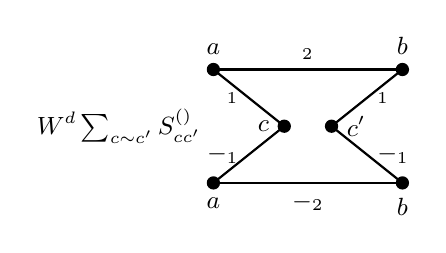
\begin{tikzpicture}[scale=1.2, every node/.style={font=\small}]

% Left graph
\coordinate (a1) at (0, 1.2);
\fill (a1) circle (2pt) node[above=2pt]{$a$};
%\node[above left] at (a1) {$a_1$};

\coordinate (a2) at (2, 1.2);
\fill (a2) circle (2pt) node[above=2pt]{$b$};

\coordinate (b) at (0.75, 0.6);
\fill (b) circle (2pt) node[left=2pt]{$c$};

\coordinate (b') at (1.25, 0.6);
\fill (b') circle (2pt) node[right=2pt]{$c'$};

\coordinate (a1') at (0, 0);
\fill (a1') circle (2pt) node[below=2pt]{$a$};

\coordinate (a2') at (2, 0);
\fill (a2') circle (2pt) node[below=2pt]{$b$};

\node at (-1,0.6) {$W^d\sum_{c\sim c'}S_{cc'}^{(\sB)}$};

\draw[thick] (a1) -- (b) node[midway, left] {$\sig_1$};
 \draw[thick] (b') -- (a2) node[midway, right] {$\sig_1$};
\draw[thick] (b') -- (a2') node[midway, right] {$-\sig_1$};
 \draw[thick] (b) -- (a1') node[midway, left] {$-\sig_1$};
\draw[thick] (a1) -- (a2) node[midway, above] {$\sig_2$};
\draw[thick] (a1') -- (a2') node[midway, below] {$-\sig_2$};
% \draw[decorate, decoration={snake, amplitude=0.4mm, segment length=2mm}, thick] (b) -- (b')
% node[midway, above] {$S^{(\sB)}$};

% Right graph
% \node (a1r) at (6, 2) {$\bullet$};
% \node[above left] at (a1r) {$[a_1]$};

% \node (a2r) at (10, 2) {$\bullet$};
% \node[above right] at (a2r) {$[a_2]$};

% \node (br) at (7.5, 1) {$\bullet$};
% \node[below] at (br) {$[b]$};

% \node (b'r) at (8.5, 1) {$\bullet$};
% \node[below] at (b'r) {$[b]$};

% \node (a1r') at (6, 0) {$\bullet$};
% \node[below left] at (a1r') {$[a_1']$};

% \node (a2r') at (10, 0) {$\bullet$};
% \node[below right] at (a2r') {$[a_2']$};

% \draw[thick] (a1r) -- (br) node[midway, left] {$-$};
%  \draw[thick] (b'r) -- (a2r) node[midway, right] {$-$};
% \draw[thick] (b'r) -- (a2r') node[midway, right] {$+$};
%  \draw[thick] (br) -- (a1r') node[midway, left] {$+$};
% \draw[thick] (a1r) -- (a2r) node[midway, above] {$+$};
% \draw[thick] (a1r') -- (a2r') node[midway, below] {$-$};
% \draw[decorate, decoration={snake, amplitude=0.4mm, segment length=2mm}, thick] (br) -- (b'r)
%         node[midway, above] {$S^{(B)}$};
        
\end{tikzpicture}}
}
\end{equation}
Each solid edge between two block vertices (e.g., $a$ and $b$) with charge $\sig\in\{+,-\}$ denotes a resolvent entry $(G_t(\sig))_{xy}$ or $(G_t(\sig))_{yx}$ with $x\in [a]$ and $y\in [b]$. The orientation of the graph is assumed to be clockwise.
To illustrate the idea for the proof of \eqref{eq:MG_conclusion}, assume without loss of generality that the vertex $c$ is closer to $b$ than to $a$. Then, the graph in \eqref{eq:2martingale_quad} already contains four ``long legs'': in addition to the two edges connecting $a$ and $b$, the two edges connecting $a$ and $c$ contribute a factor $\Psi_t^2(|a-c|) \le \Psi_t^2(|a-b|/2) \lesssim \Psi_t^2(|a-b|)$. Summing over the two remaining edges connected to $c'$ and applying Cauchy--Schwarz together with Ward's identity yields an additional factor of $\eta_t^{-1}$.
However, compared with the target estimate \eqref{eq:MG_conclusion}, we still miss the factor $\Psi_t(0)$. To recover it, we require a sharper treatment of the 6-$G$-loop that avoids applying Cauchy--Schwarz directly to the two edges connected to $c'$. Indeed, if we can directly perform the global summation over these two edges without taking absolute values, Ward's identity \eqref{eq_Ward0} produces a solid edge, which contributes the desired small factor $\Psi_t(0)$.
This is precisely achieved via the following \emph{$\contract$ inequality} for the 6-$G$-loop in \eqref{eq:2martingale_quad}, which can be regarded as a pointwise version of the more general $\contract$ inequality \eqref{u2jzooi-2} below.
For simplicity, we abbreviate $G\equiv G_t$ in the following proof. 


\begin{lemma} [$\Contract$ inequality]\label{ygdhmsgq0}
For any subset $\cal A\subset \Zn$, we have that 
%The symmetric 6-loop in \eqref{eq_mart-sum} satisfies the bound 
\begin{equation}\label{eq_sym_loop_bound}
\sum_{c'\in \cal A}\sum_{c\sim c'} \mathcal{L}^{(6)}_{t, (\bsig\otimes \overline\bsig)^{(1)}, \ba(c,c')} \lesssim \frac{1}{W^d\eta_t}\max_{c'\in \cal A}\left(\mathcal{L}^{(4)}_{t,\bsig^{(\alt)}, (c',b,c',b)}\right)^{1/2}\cdot \max_{\sig\in\{+,-\}} \big|\mathcal{L}^{(3)}_{t, (\sigma,\sig_2,-\sig_2), (a,b,a)} \big| ,
\end{equation}
where $\bsig^{(\alt)}=(\sig_1,-\sig_1,\sig_1,-\sig_1)$ is an alternating loop. By symmetry, a similar inequality holds: % with $\wt{\bsig}' = (-{\sigma}_1, -{\sigma}_2, \sigma_2, \sigma_1)$:
\begin{equation}\label{eq_sym_loop_bound2}
 \sum_{c\in \cal A}\sum_{c'\sim c}\mathcal{L}^{(6)}_{t, (\bsig\otimes \overline\bsig)^{(1)}, \ba(c,c')} \lesssim \frac{1}{W^d\eta_t}\max_{c\in \cal A} \left(\mathcal{L}^{(4)}_{t,\bsig^{(\alt)}, (a,c,a,c)}\right)^{1/2} \cdot \max_{\sig\in \{+,-\}}\big|\mathcal{L}^{(3)}_{t, (\sig, -{\sigma}_2, \sigma_2), (b,a,b)}\big|.
\end{equation}
\end{lemma}
\begin{proof}

We only prove the inequality \eqref{eq_sym_loop_bound}, while the proof of \eqref{eq_sym_loop_bound2} is similar by switching the roles of $(a,c)$ and $(b,c')$. We view the symmetric $6$-loop as a quadratic form. For any $c,c'\in \Zn$ with $|c-c'|\le 1$ and any $z\in [c]$, we define the column vector \smash{$\psi^{z}\in \C^{W^d}$} and the $W^d\times W^d$ matrix \smash{$A^{(c')}$} as
\begin{align*}
    \psi^{z}_{y} &=  (G(\sig_1)E_aG(\sig_2))_{zy}, \ \ \forall y\in [b], \quad \text{and}\quad 
    A^{(c')}_{y_1  y_2} = (G(\sig_1)E_{c'} G(-\sig_1))_{y_1 y_2}, \ \ \forall y_1, y_2 \in [b].
%    W^{-d} \sum_{z'\in \cal [c']} G_{y_1 z'}(\sig_1) G_{z'y_2}(-\sig_1), \quad \forall y_1, y_2 \in [b].
\end{align*}
% For any $z\in \mathcal{I}_c$, define the column vector $\psi^z$ and and a Hermitian matrix $A$ as follows.
% \begin{align*}
%     \psi^{z}_{y} &= W^{-d}\sum_{x\in\mathcal{I}_a}G^\ast_{zx}G_{xy}, \quad y\in \mathcal{I}_b, \\
%     A_{y_1  y_2} & = W^{-d} \sum_{z'\in \mathcal{I}_{c'}} G_{y_1 z'} G^\ast_{z'y_2}, \quad y_1, y_2 \in\mathcal{I}_b.
% \end{align*}
Then, each summand on the left-hand side (LHS) of \eqref{eq_sym_loop_bound} can be written as
\begin{equation}\label{eq_6loop_quadform}
\mathcal{L}^{(6)}_{t, (\bsig\otimes \overline\bsig)^{(1)}, \ba(c,c')} = W^{-3d} \sum_{z\in[c]} \left(\psi^{z}\right)^\ast A^{(c')} \psi^{z} \le W^{-3d} \|A^{(c')}\|  \sum_{z\in[c]} \|\psi^{z}\|_2^2.
\end{equation}
Since the operator norm of $A^{(c')}$ is bounded above by its Hilbert-Schmidt norm, we have
\begin{equation}\label{eq:L4loop}
    \|A^{(c')}\|^2 \le \sum_{y_1,y_2\in [b]} (G(\sig_1)E_{c'} G(-\sig_1))_{y_1y_2} (G (\sig_1)E_{c'}G(-\sig_1))_{y_2 y_1} =: W^{2d} \mathcal{L}^{(4)}_{t,\bsig^{(\alt)}, (c',b,c',b)}.
\end{equation}
On the other hand, the sum of the squared $L^2$-norms of $\psi^z$ is equal to
\begin{equation*}
    \sum_{z\in[c]} \|\psi^{z}\|_2^2 =  \sum_{z\in\cal [c],y\in [b]} (G(\sig_1)E_a G(\sig_2))_{z y} (G(-\sig_2)E_a G(-\sig_1))_{y z} = W^{2d} \mathcal{L}^{(4)}_{t, \bsig', (a,b,a,c)},
\end{equation*}
where $\bsig' = (\sigma_1, \sigma_2, -{\sigma}_2, -{\sigma}_1)$. Plugging the previous two displays into \eqref{eq_6loop_quadform} yields 
\begin{align}\label{eq_sym_loop_bound_old}
 \mathcal{L}^{(6)}_{t, (\bsig\otimes \overline\bsig)^{(1)}, \ba(c,c')} \le \left(\mathcal{L}^{(4)}_{t,\bsig^{(\alt)}, (c',b,c',b)}\right)^{1/2} \cdot \mathcal{L}^{(4)}_{t, \bsig', (a,b,a,c)} .
\end{align}
Summing this inequality over $c'\in \cal A$ and $c\sim c'$, we obtain 
\begin{align*}
\sum_{c'\in \cal A}\sum_{c\sim c'} \mathcal{L}^{(6)}_{t, (\bsig\otimes \overline\bsig)^{(1)}, \ba(c,c')} &\lesssim \max_{c'\in \cal A}\left(\mathcal{L}^{(4)}_{t,\bsig^{(\alt)}, (c',b,c',b)}\right)^{1/2}\cdot \sum_{c}\mathcal{L}^{(4)}_{t, \bsig', (a,b,a,c)} ,
\end{align*}
where the summation over $c$ has been extended to all of $\Zn$, at the cost of a dimensional constant, since each $c$ has at most $3^d$ neighbours $c'$. Finally, applying Ward's identity \eqref{WI_calL} to the sum over $c$ yields the desired bound \eqref{eq_sym_loop_bound}. 
\end{proof}



Now, we are ready to complete the proof of \Cref{lem: EMn2_N}. We first prove the bound \eqref{eq:MG_conclusion}. We split the summation over $c$ into two regions according to the distances from $c$ to the fixed indices $a$ and $b$: 
\begin{equation}\label{eq:S1+S2}
    (\mathcal{E} \otimes \mathcal{E})_{t, \bsig, \boldsymbol{a}, \boldsymbol{a}}^M \lesssim  W^d \sum_{\substack{c'\sim c \\ |c-b|> |c-a|}}  \mathcal{L}^{(6)}_{t, (\bsig\otimes \overline\bsig)^{(1)}, \ba(c,c')} + W^d \sum_{\substack{c'\sim c\\ |c-b|\le |c-a|}} \mathcal{L}^{(6)}_{t, (\bsig\otimes \overline\bsig)^{(1)}, \ba(c,c')} =: \mathcal{S}_1 + \mathcal{S}_2.
\end{equation}
By symmetry, it suffices to prove the bound \eqref{eq:MG_conclusion} for the sum $\mathcal{S}_1$ using \eqref{eq_sym_loop_bound}. (To control the sum $\cal S_2$, we only need to utilize the inequality \eqref{eq_sym_loop_bound2} in place of \eqref{eq_sym_loop_bound} in the following proof.) 
%In this case, by triangle inequality, we have that $|c-b|\ge |a-b|/2$. 
% We split the summation in \eqref{eq_mart-sum} into two parts as follows. Since $c\sim c'$, by triangle inequality we either have $|a-c|\ge |a-b|/3$ or $|c'-b| \ge |a-b|/3$. Since all of the terms in \eqref{eq_mart-sum} are non-negative, we have
% \begin{equation*}
%     (\mathcal{E} \otimes \mathcal{E})_{t, \bsig, \boldsymbol{a}, \boldsymbol{a}}^M \lesssim W^d \sum_{\substack{c\sim c'\\ |c'-b| \ge |a-b|/3}} \mathcal{L}^{(6)}_{t, \bsig', abc'abc} + W^d \sum_{\substack{c\sim c'\\ |c-a| \ge |a-b|/3}} \mathcal{L}^{(6)}_{t, \bsig', abc'abc} =: \mathcal{S}_1 + \mathcal{S}_2.
% \end{equation*}
%Without loss of generality, it suffices to show the bound \eqref{eq:MG_conclusion} for the sum $\mathcal{S}_1$. 
Under the conditions \(|c-c'|\le 1\) and \(|c-b| \ge |a-b|/2\), we bound each off-diagonal $G$-entry of the $4$-loop \smash{$\mathcal{L}^{(4)}_{t,\bsig^{(\alt)}, (c',b,c',b)}$} using \eqref{GijGEX}, and each diagonal $G$-entry using \eqref{GiiGEX}. This gives
\begin{align}\label{eq:pointwise_loop}
\p{ \mathcal{L}^{(4)}_{t,\bsig^{(\alt)}, (c',b,c',b)}}^{1/2} &\prec  \max_{\substack{|b'-b|\le 1,|c''-c'|\le 1,\\ \bsig\in \{(+,-),(-,+)\}}}\mathcal{L}^{(2)}_{t,\bsig, (b',c'')}+W^{-d}\mathbf 1_{|b-c'|\le 1}\prec \Psi_t^2(|b-c'|) \lesssim \Psi_t^2(|a-b|).
\end{align}
Here, the second step uses the assumption \eqref{eq:LW_assm} on the 2-loops together with condition \eqref{eq:Psi}, while the third step follows from $|c-c'|\le 1$, $|c-b|\ge |a-b|/2$, and another application of \eqref{eq:Psi}. Plugging this bound into the $\contract$ inequality \eqref{eq_sym_loop_bound}, we get that
\begin{equation}\label{eq:reduce4to3}
    \mathcal{S}_1 \prec \frac{1}{\eta_t} \Psi_t^2\left(|a-b|\right) \max_{\sig\in\{+,-\}}\left|\mathcal{L}^{(3)}_{t, (\sig,\sig_2,-\sig_2), (a,b,a)}\right|.
\end{equation}
To bound the 3-$G$-loop on the RHS, we write
\[\mathcal{L}^{(3)}_{t, (\sig,\sig_2,-\sig_2), (a,b,a)}=W^{-3d}\sum_{x,x'\in [a]}\sum_{y\in[b]}G_{xx'}(\sig)G_{x'y}(\sig_2)G_{yx}(-\sig_2), \]
and apply an argument analogous to that in \eqref{eq:pointwise_loop}, obtaining 
\begin{align}
\big| \mathcal{L}^{(3)}_{t, (\sig,\sig_2,-\sig_2), (a,b,a)}\big|& \prec \Psi_t(0) \cdot \Psi_t^2(|a-b|).\label{eq:reduce4_bdd3}
\end{align} 
Roughly speaking, the factor $ \Psi_t^2(|a-b|)$ arises from the two long legs---namely, the entries $G_{x'y}$ and $G_{yx}$ between $[a]$ and $[b]$. The short leg $G_{xx'}$, with both indices in $[a]$, contributes a factor of $\Psi_t(0)+W^{-d}$ by \eqref{GiiGEX}. (More precisely, each off-diagonal entry of $G$ contributes a factor of $\Psi_t(0)$, while diagonal entries contribute $W^{-d}$.) Substituting \eqref{eq:reduce4_bdd3} into \eqref{eq:reduce4to3} gives the desired bound \eqref{eq:MG_conclusion}.



In order to show the bound \eqref{eq:MG_conclusion3}, we define two cutoff scales 
\be\label{eq:cutoff_scales}
\ell_t^\ast = (\log W)^{3/2}\ell_t,\quad \ell_t^{\dag} = (\log W)^{7/4}\ell_t.\ee
Then, we divide the proof into two cases. 
First, suppose $|a-b| \le \ell_t^{\dag}$. In this case, the function $\widetilde{\mathcal{T}}^{\ell}_{t,D}\p{|a-b|}$ exhibits no exponential decay. Hence, it suffices to apply the polynomial decay bound \eqref{eq:MG_conclusion2} with $c_0=d$ and $K=\ell$, i.e.\ with the \emph{truncated} profile function \smash{\(\Psi_t(r) = (W^{-d} B_{t, r\wedge \ell})^{1/2}.\)}  
The conclusion \eqref{eq:MG_conclusion3} then follows directly from \eqref{eq:MG_conclusion2} and the facts 
\[
\br{\Psi_t(r)}^2 \prec  W^{-d}\widetilde{\mathcal{T}}^{\ell}_{t,D}\p{r} , \quad W^{-d}\widetilde{\mathcal{T}}^{\ell}_{t,D}\p{r} \prec \br{\Psi_t(r)}^2, \quad \forall \ 0\le r\le \ell_t^\dag,
\]
both of which hold by the definition \eqref{defWTTlD} of \smash{$\wT^{\ell}_{t,D}$}, since ${\cal T}_{t}(\rho)\asymp B_{t,\rho}\exp(-(\rho/\ell_t)^{1/2})$ and $\exp(-(\rho/\ell_t)^{1/2})\ge W^{-\oo(1)}$ for $0\le \rho\le \ell\wedge \ell_t^\dag$. We stress that the truncation is needed here: for the untruncated profile $(W^{-d}B_{t,r})^{1/2}$ the second bound fails in the range $\ell<r\le \ell_t^\dag$, where \smash{$\wT^{\ell}_{t,D}(r)={\cal T}_t(\ell)$} while $B_{t,r}\ll B_{t,\ell}$.
It remains to deal with the case 
\be\label{eq:largea-b}|a-b| > \ell_t^{\dag} = (\log W)^{7/4}\ell_t.\ee 
In this case, we split the summation \eqref{eq_mart-sum} into three parts as follows: 
\begin{align}
    (\mathcal{E} \otimes \mathcal{E})_{t, \bsig, \boldsymbol{a}, \boldsymbol{a}}^M &\lesssim W^d \bigg(\sum^\star_{\substack{|c-a| \le \ell_t^\ast \text{ or } |c'-b| > \ell}} + \sum^\star_{\substack{|c'-b| \le \ell_t^\ast \text{ or } |c-a| > \ell}} + \sum^\star_{\substack{\ell_t^\ast < |c'-b|,|c-a| \le \ell}}\bigg) \mathcal{L}^{(6)}_{t, (\bsig\otimes \overline\bsig)^{(1)}, \ba(c,c')}\nonumber\\
    &=: \widetilde{\mathcal{S}}_1 + \widetilde{\mathcal{S}}_2 + \widetilde{\mathcal{S}}_3.\label{eq;S123}
\end{align}
where $\sum^\star$ refers to the summation subject to the constraint $|c-c'|\le 1$. 
To estimate $\widetilde{\mathcal{S}}_1$, we combine \eqref{GijGEX} with \eqref{eq:LW_assm_exp} and proceed analogously to \eqref{eq:pointwise_loop}. This yields  
\begin{align}\label{eq:pointwise_loop2}
    \p{ \mathcal{L}^{(4)}_{t,\bsig^{(\alt)}, (c',b,c',b)}}^{1/2} \prec W^{-d}\wT_{t,D}^{\ell}(|b-c'|) \prec W^{-d}\wT_{t,D}^{\ell}(|a-b|),
\end{align}
where the second inequality is justified as follows: (1) if $|c'-b|>\ell$, then \smash{\(\wT_{t,D}^{\ell}(|b-c'|) = \wT_{t,D}^{\ell}(\ell)\le \wT_{t,D}^{\ell}(|a-b|);\)} (2) if $|c-a|\le \ell_t^*$, then by \eqref{eq:largea-b}, we have $|b-c'|\ge |a-b|-(\ell_t^*+1) =(1-\oo(1))|a-b|$, which implies 
\[ \wT_{t,D}^{\ell}(|b-c'|) \le \wT_{t,D}^{\ell}\p{|a-b|-(\ell_t^*+1)} \prec \wT_{t,D}^{\ell}(|a-b|). \]
Substituting \eqref{eq:pointwise_loop2} into the $\contract$ inequality \eqref{eq_sym_loop_bound}, we obtain  
\begin{align}
    \widetilde{\mathcal{S}}_1 &\prec  \frac{1}{\eta_t} \left[W^{-d} \widetilde{\mathcal{T}}^{\ell}_{t,D}\p{|a-b|}\right] \max_{\sig\in\{+,-\}}\left|\mathcal{L}^{(3)}_{t, (\sig,\sig_2,-\sig_2), (a,b,a)}\right|.\label{eq_S1tilde}
\end{align}
Next, using \eqref{GijGEX} and \eqref{eq:LW_assm_exp}, we obtain a similar bound on the 3-$G$-loop as in \eqref{eq:reduce4_bdd3}:
\[\left|\mathcal{L}^{(3)}_{t, (\sig,\sig_2,-\sig_2), (a,b,a)}\right|\prec (W^{-d}B_{t,0})^{1/2}\cdot W^{-d} \widetilde{\mathcal{T}}^{\ell}_{t,D}\p{|a-b|}.\]
Plugging this into \eqref{eq_S1tilde} gives
\begin{equation}\label{eq:boundwtS_1}
    \widetilde{\mathcal{S}}_1 \prec \frac{1}{\eta_t} \left(W^{-d}B_{t,0}\right)^{1/2}\left[W^{-d} \widetilde{\mathcal{T}}^{\ell}_{t,D}\p{|a-b|}\right]^2 , 
\end{equation}
which is controlled by the RHS of \eqref{eq:MG_conclusion3}. By symmetry, an identical bound holds for $\wt {\cal S}_2$.


% Since, all terms on the right-hand side are bounded by large constant powers of $W$ and the control parameters $B_{t,0}$, $\widetilde{\mathcal{T}}^{\ell,D}_{t,|a-b|}$ are bounded below by constant powers of $W$, the constant $\tilde{D}$ can be chosen large enough, such that
% \begin{equation*}
%      \widetilde{\mathcal{S}}_1 \prec \frac{1}{\eta_t} \left[\left(W^{-d}B_{t,0}\right)^{1/2} + \left(W^{-d}B_{t,0}\right)^{1/2}\left(\mathcal{J}^{\ell,D}_{t}\right)^2\right] \cdot \left(W^{-d} \widetilde{\mathcal{T}}^{\ell,D}_{t,|a-b|}\right)^2.
% \end{equation*}

It remains to control the sum $\widetilde{\mathcal{S}}_3$. In this case, we bound all legs of the original $6$-loop directly using \eqref{GijGEX}. Here, all legs of this loop have lengths (i.e., $|a-b|$, $|a-c|$, and $|c'-b|$) at least $\ell_t^\ast$. Then, instead of using the assumption \eqref{eq:LW_assm_exp}, we will bound the $2$-loops using the parameter defined in \eqref{defCALJ} as follows: for any $a,b\in \Zn$ satisfying $|a-b|\gtrsim \ell_t^\ast$,  
\begin{equation}\label{eq_L2-J}
    \mathcal{L}^{(2)}_{t,(-,+),(a,b)} \prec \wh{\mathcal{J}}^{\ell}_{t,D} \cdot W^{-d} \widetilde{\mathcal{T}}^{\ell}_{t,D}\p{|a-b|} + \mathcal{K}^{(2)}_{t,(-,+),(a,b)} \lesssim \big(\wh{\mathcal{J}}^{\ell}_{t,D} +W^{-D}\big)\cdot W^{-d} \widetilde{\mathcal{T}}^{\ell}_{t,D}\p{|a-b|} ,
\end{equation}
where the second step is due to the exponential decay of the 2-$\mathcal{K}$-loop given by \eqref{prop:ThfadC}. 
Then, using \eqref{GijGEX} to bound the 6 legs of the 6-loop, we obtain that 
\begin{align}
    \widetilde{\mathcal{S}}_3 \prec &~W^{-2d}\p{\wh{\mathcal{J}}^{\ell}_{t,D}+W^{-D}}^3\sum_{\substack{\ell_t^\ast < |c'-b|,|c-a| \le \ell}}^\star \widetilde{\mathcal{T}}^{\ell}_{t,D}\p{|a-b|} \widetilde{\mathcal{T}}^{\ell}_{t,D}\p{|a-c|}  \widetilde{\mathcal{T}}^{\ell}_{t,D}\p{|c-b|} ,\label{eq:boundwtS31}
\end{align}
where we also use that 
$\widetilde{\mathcal{T}}_{t,D}^{\ell}\p{|c'-b|}\asymp \widetilde{\mathcal{T}}_{t,D}^{\ell}\p{|c-b|}$ for $|c-c'|\le 1$. We can bound the RHS of \eqref{eq:boundwtS31} by
\begin{align*}
% &~W^{-2d} \left(\mathcal{J}^{\ell}_{t,D}+W^{-D}\right)^3\cdot  \widetilde{\mathcal{T}}^{\ell}_{t,D}\p{|a-b|} \sum_{\ell_t^\ast<|c-a|,|c'-b|\le \ell}^\star \widetilde{\mathcal{T}}^{\ell}_{t,D}\p{|a-c|} \widetilde{\mathcal{T}}^{\ell}_{t,D}\p{|c-b|} \\
% \lesssim 
&~\left(\wh{\mathcal{J}}^{\ell}_{t,D}+W^{-D}\right)^3\cdot W^{-2d} \widetilde{\mathcal{T}}^{\ell}_{t,D}\p{|a-b|}\cdot \sum_c \br{\mathcal{T}_{t}\p{|a-c|}+W^{-D}}\br{\mathcal{T}_{t}\p{|c-b|}+W^{-D}} \\
\lesssim &~\frac{(\wh{\mathcal{J}}^{\ell}_{t,D}+W^{-D})^3}{1-t} \cdot W^{-2d} \widetilde{\mathcal{T}}^{\ell}_{t,D}\p{|a-b|}\cdot \br{\mathcal{T}_{t}\p{|a-b|} +W^{-D}}\lesssim \frac{(\wh{\mathcal{J}}^{\ell}_{t,D}+W^{-D})^3}{\eta_t} \cdot \left(W^{-d} \widetilde{\mathcal{T}}^{\ell}_{t,D}\p{|a-b|}\right)^2,
\end{align*}
where we use \eqref{TTT2} and the fact $\sum_{a}\cal T_t\p{|a|}\lesssim (1-t)^{-1}$. This finishes the estimation of \smash{$\wt{\cal S}_3$}, and hence completes the proof of the bound \eqref{eq:MG_conclusion3}.

%We expand the RHS of \eqref{eq:boundwtS31} and notice that by choosing $D'$ sufficiently large depending on $D$, we can guarantee that each term containing the factor $W^{-D'}$ will be controlled by the RHS of \eqref{eq:MG_conclusion3}. 
%Note that replacing $c'$ by $c$ here is harmless, because $\widetilde{\mathcal{T}}^{\ell,D}_{t,|c'-b|}\prec \widetilde{\mathcal{T}}^{\ell,D}_{t,|c-b|}$. Similarly to the bound on $\widetilde{\mathcal{S}}_1$ above, we can ignore the terms involving $W^{-\tilde{D}}$, because $\tilde{D}$ can be chosen large enough to have these terms consumed by $\eta_t^{-1}\left(W^{-d}B_{t,0}\right)^{1/2}\left(W^{-d} \widetilde{\mathcal{T}}^{\ell,D}_{t,|a-b|}\right)^2$. 
%For the main term, we bound it by  %$\widetilde{\mathcal{T}}^{\ell,D}_{t,|a-c|}$ and $\widetilde{\mathcal{T}}^{\ell,D}_{t,|c-b|}$ by $\mathcal{T}_{t,|a-c|}$ and $\mathcal{T}_{t,|c-b|}$ taking into account that $|c-a|, |c-b| \le \ell$ and then extend the summation over $c$ to the entire space $\Z_L^d$. This allows us to apply \eqref{TTT2} as follows

%\end{proof}
 

 

 
\section{Steps 3 and 4: Sharp maximum estimates for \texorpdfstring{$G$}{G}-loops}\label{Sec:Steps34}


In this section, we apply the integrated loop hierarchy \eqref{int_K-LcalE} to complete the proofs of Steps 3 and 4. The key task is to show that the second through fifth terms in \eqref{int_K-LcalE} are errors in the max-norm sense.

The integrands in the second to fourth terms on the RHS of \eqref{int_K-LcalE} each involve a global sum over an index of an $\cal L$- or $(\cL-\cK)$-loop (see \eqref{DefKsimLK}, \eqref{def_ELKLK}, and \eqref{def_EwtG}). In low dimensions $d\in \{1,2\}$, these terms can be controlled directly using their max-norms, together with a factor $\ell_t^d$ that captures the range of exponential decay.
For $d\in\{1,2\}$, the factor $\ell_t^d$ is bounded by $|1-t|^{-1}$, which incurs only a harmless logarithmic contribution upon integration in time. However, in higher dimensions $d\ge 3$, an additional factor $\ell_t^{d-2}$ arises on top of the $(1-t)^{-1}$, creating a substantial term that cannot be canceled. 
To obtain sufficiently sharp bounds without relying on the precise pointwise decay of higher-order $G$-loops, we develop a new \emph{$\contract$ inequality} \eqref{yi2oslxj2}, derived from the Cauchy--Schwarz inequality and the Ward's identities \eqref{WI_calL} and \eqref{WI_calK}. Although technically simple, this inequality provides a powerful tool: it allows us to control the absolute sum of a higher-order $G$-loop in terms of lower-order ones in a sharp max-norm sense, and crucially produces the desired $(1-t)^{-1}$ factor without introducing any excess powers of $\ell_t$.
Among all these terms, one remains that cannot be effectively controlled using the $\contract$ inequalities---namely, the term of the form $(\cal L-\cal K)^{(2)}\diamond(\cal L-\cal K)^{(n)}$ (recall the notation in \eqref{eq:diamond}) in \eqref{def_ELKLK}. This term is instead shown to be an error by applying the pointwise $(\cal L-\cal K)^{(2)}$-estimate \eqref{Eq:Gdecay_w}.


Bounding the martingale term requires controlling a $(2n+2)$-loop (recall \Cref{def:CALE}). The corresponding loop structure is symmetric and involves two summation indices along the loop (see e.g., \eqref{eq:2martingale_quad}). To handle it, we derive another $\contract$ inequality \eqref{u2jzooi-2}, obtained by extending the argument in the proof of \Cref{ygdhmsgq0}. This inequality yields a non-sharp but sufficient bound for the martingale term, introducing an additional power of $W$, i.e., the factor $(W^{-d}B_{t,0})^{-1/(2p)}$ in \eqref{eq:MG_nloop}. However, this factor remains small enough for our proof for large enough $p$.


Our overall strategy for Steps 3 and 4 can now be summarized as follows. Using the $\contract$ inequalities together with a good stability estimate \eqref{Eq:Gdecay_w} for $({\cal L}-{\cal K})^{(2)}$-loops, we can bound each term in \eqref{int_K-LcalE} either by lower-order $(\cL-\cK)$-loops or by higher-order $(\cL-\cK)$-loops with an extra small factor $W^{-\varepsilon}$. Then, with the integrated hierarchy \eqref{int_K-LcalE}, we can bootstrap from a sequence of weaker bounds to tighter ones, ultimately yielding improved control on the entire hierarchy of $(\cL -\cK)$-loops in each induction. As in \cite{YY_25, DYYY25, erdHos2025zigzag}, after $\OO(1)$ iterations, this process yields (almost) sharp max-norm bounds for all $(\cL-\cK)$-loops.



%\subsection{Ward's inequality and estimation of the loop hierarchy}


%The proofs of Steps 3 and 4 rely crucially on the following (maximum) Ward's inequalities. % which are consequences of the Ward's identities \eqref{WI_calL} and \eqref{WI_calK}. %The second Ward's inequality \eqref{u2jzooi-2} is essential to bound the quadratic variation of the martingale term $\mathcal{E}^{M,(n)}$. It is a generalized $G$-loop version of the bound used in Lemma 10 of \cite{DY} to control the term $\mathcal{E}^{M,(2)}$.  

\begin{lemma} [$\Contract$ inequality]\label{ygdhmsgq}
For each $1\le k \le n-1$, we have the bound
\begin{align}\label{yi2oslxj2}
  \max_{\bsig}\sum_{a_n} |{\cal L}^{(n)}_{t, \bsig, \ba}|\le \frac 1 {W^{d}\eta_t} \left(\max_{\bsig,\mathbf{b}}  \left|{\cal L}^{(2k-1)}_{t, \bsig, \mathbf{b}}\right|\cdot \max_{\bsig,\mathbf{b}}  \left|{\cal L}^{(2n-2k-1)}_{t, \bsig, \mathbf{b} }\right|\right)^{\frac 1 2}   .
\end{align}
Furthermore, for any $n\ge 4$, $1\le k<j<l\le n-1$, and subsets $\cal A(a_n)\subset \Zn$ (which may depend on $a_n$) of cardinality $|\cal A(a_n)|\le C$ for a constant $C>0$, the following bound holds for any fixed $p\ge 1$: 
\begin{align}\label{u2jzooi-2}
   \max_{\bsig} \sum_{a_n}\sum_{a_j\in \cal A(a_n)} |{\cal L}^{(n)}_{t,\bsig, {\ba}}|\le  &~\frac{C}{W^d\eta_t} \left(\max_{\bsig,\mathbf{b}}  \left|{\cal L}^{(2k-1)}_{t, \bsig, \mathbf{b}}\right|\cdot \max_{\bsig,\mathbf{b}}  \left|{\cal L}^{(2n-2l-1)}_{t,\bsig,\mathbf{b}}\right|\right)^{\frac 1 2}   \left(\max_{\bsig,\bfb}   \left|{\cal L}^{(2(l-k)p)}_{t,\bsig, \mathbf b}\right|\right)^{\frac1{2p}} .
\end{align}
\end{lemma}

\begin{proof}%[Proof of lemma \ref{ygdhmsgq}]
We first prove \eqref{yi2oslxj2}.  Applying the Cauchy-Schwarz inequality with respect to the averages over $[a_k]$ and $[a_n]$ in the loop \smash{${\cal L}^{(n)}_{t,\bsig, \ba}$}, we obtain that for $\bsig=(\sig_1,\ldots, \sig_n)$ and $\ba=(a_1,\ldots, a_n)$, 
\begin{align}\label{eq:CS1}
     |{\cal L}^{(n)}_{t, \bsig,\ba}| 
     \; \le \;&
     \left({\cal L}^{(2k)}_{t,\bsig_1,\ba_1 }\cdot  {\cal L}^{(2n-2k)}_{t,\bsig_2,\ba_2}\right)^{1/2},
     \end{align}
where $\ba_1$, $\ba_2$, $\bsig_1$, and $\bsig_2$ are defined as     
 \begin{align}
    {\ba}_1= (a_1,\cdots, a_{k-1}, a_k, a_{k-1},\cdots ,a_1,a_n), &\quad 
    \bsig_1 = (\sigma_1, \cdots, \sigma_{k}, -{\sigma_{k}},\cdots, -\sigma_1) ,\nonumber
     \\\nonumber
    {\ba}_2= (a_{n-1},\cdots, a_{k+1}, a_k, a_{k+1}, \cdots ,a_{n-1},a_n), &\quad 
    \bsig_2 = (-{\sigma_n}, \cdots, -\sig_{k+1}, \sigma_{k+1}, \cdots ,\sigma_n).
\end{align}  
Note that the loops ${\cal L}^{(2k)}_{t,\bsig_1,{\ba}_1}$ and ${\cal L}^{(2n-2k)}_{t, \bsig_2,{\ba}_2}$ are both non-negative since $\bsig_1$ and $\bsig_2$ are symmetric.  Then, applying the Cauchy-Schwarz inequality to \eqref{eq:CS1} again, we obtain that 
\be\label{eq;genWard0}
      \sum_{a_n} |{\cal L}^{(n)}_{t, \bsig,\ba}| \le  
     \Big(\sum_{a_n}{\cal L}^{(2k)}_{t, \bsig_1,\ba_1}\Big)^{1/2} \Big(\sum_{a_n}{\cal L}^{(2n-2k)}_{t, \bsig_2,\ba_2}\Big)^{1/2}.
\ee
Using Ward's identity \eqref{WI_calL}, we can express the $G$-loops on the RHS as  
\be\label{eq;genWard1}
\sum_{a_n}{\cal L}^{(2k)}_{t, \bsig_1,\ba_1} =\frac{{\cal L}^{(2k-1)}_{t, \bsig^+_1,\ba'_1}
-{\cal L}^{(2k-1)}_{t, \bsig^-_1,\ba'_1}}{2\ii W^d\eta_t} ,\quad
\sum_{a_n}{\cal L}^{(2n-2k)}_{t, \bsig_2,\ba_2} =\frac{{\cal L}^{(2n-2k-1)}_{t, \bsig^+_2,\ba'_2}
-{\cal L}^{(2n-2k-1)}_{t, \bsig^-_2,\ba'_2}}{2\ii W^d\eta_t},
\ee
where $\ba'_1$, $\ba'_2$, $\bsig^{\pm}_1$, and $\bsig^{\pm}_2$ are defined as 
\begin{align*}
\ba'_1=(a_1,\cdots, a_{k-1}, a_k, a_{k-1}\cdots, a_1),\quad &\bsig^{\pm}_1 = ( \pm,\sigma_2, \cdots, \sigma_{k}, -{\sigma_{k}},\cdots,-{\sigma_2}), \\
\ba'_2=( a_{n-1}\cdots,   a_{k+1}, a_{k}, a_{k+1},\cdots, a_{n-1}), \quad 
    &\bsig^{\pm}_2 = (\pm, -{\sigma_{n-1}}, \cdots, - \sigma_{k+1}, \sigma_{k+1},\cdots  \sigma_{n-1}).
\end{align*}
Plugging \eqref{eq;genWard1} into \eqref{eq;genWard0}, we  conclude \eqref{yi2oslxj2}. 

For $\bsig=(\sigma_1,  \ldots, \sigma_n)\in \{+,-\}^n$ and \smash{$\ba = (a_1, \ldots, a_{n-1})\in (\Zn)^{n-1}$}, denote a $G$-chain of length $n$ by 
\begin{equation}\label{defC=GEG}
    {\cal C}^{(n)}_{t, \bsig, \ba} = \prod_{i=1}^{n-1}\left(G_t(\sigma_i) E_{a_i}\right)\cdot  G_t(\sigma_n) .
\end{equation}
To show \eqref{u2jzooi-2}, we split the loop ${\cal L}^{(n)}_{t, \bsig, \ba}$ at $a_k$, $a_l$, and $a_n$, and write it as 
$${\cal L}^{(n)}_{t, \bsig, \ba} = W^{-3d}\sum_{x_k\in\br{a_k} }\sum_{x_l\in\br{a_l}} \sum_{x_n\in \br{a_n}} \p{{\cal C}^{(k)}_{t, \bsig_1, \ba_1}}_{x_n x_k}\p{{\cal C}^{(l-k)}_{t, \bsig_2, \ba_2}}_{x_kx_l}\p{{\cal C}^{(n-l)}_{t, \bsig_3, \ba_3}}_{x_lx_n} ,$$
where $\ba_1=(a_1,\ldots,a_{k-1})$, $\bsig_1=(\sig_1,\ldots,\sig_k)$, $\ba_2=(a_{k+1},\ldots,a_{l-1})$, $\bsig_2=(\sig_{k+1},\ldots,\sig_l)$, $\ba_3=(a_{l+1},\ldots,a_{n-1})$, and $\bsig_3=(\sig_{l+1},\ldots,\sig_n)$. We can bound the RHS by using the operator norm of the $W^d\times W^d$ matrix $A=(A_{xy}:x\in  \br{a_k}, y\in \br{a_l})$ with \smash{$A_{xy}= ({\cal C}^{(l-k)}_{t, \bsig_2, \ba_2})_{xy}$}:
\begin{align}
    \left|{\cal L}^{(n)}_{t, \bsig, \ba}\right|\le 
\frac{1}{W^{2d}}\sum_{x_n\in \br{a_n}}
\bigg(\sum_{x_k\in \br{a_k}}\Big|\p{{\cal C}^{(k)}_{t, \bsig_1, \ba_1}}_{x_n x_k}\Big|^2\bigg)^{1/2}
\bigg(\sum_{x_l\in \br{a_l}}\Big|\p{{\cal C}^{(n-l)}_{t, \bsig_3, \ba_3}}_{x_l x_n}\Big|^2\bigg)^{1/2} \cdot \frac{1}{W^d}\|A\| .\label{eq:Apsipsi}
\end{align}
To control the operator norm $\|A\|$, we use the simple linear algebra fact 
\(\|A\|\le \left\{\tr[(AA^*)^p]\right\}^{\frac{1}{2p}} \)
for any $p\in \N$, which gives that  
\begin{align}\label{eq:Apsipsi1}
\frac{1}{W^d}\|A\| \le  \left\{\frac{1}{W^{2pd}}\tr \br{\left(AA^*\right)^{p}}\right\}^{\frac1{2p}}
\le \left(\max_{\bsig,\bfb}   \left|{\cal L}^{(2(l-k)p)}_{t, \bsig , \bfb}\right|\right)^{\frac1{2p}}
\end{align}
Plugging \eqref{eq:Apsipsi1} into \eqref{eq:Apsipsi} and applying the Cauchy--Schwarz inequality, we obtain that 
\begin{align*}
 \sum_{a_n}\sum_{a_j\in \cal A(a_n)} \left|{\cal L}^{(n)}_{t, \bsig, \ba}\right|&\le C  \left(\max_{\bsig,\bfb}  \left| {\cal L}^{(2(l-k)p)}_{t, \bsig, \bfb}\right|\right)^{\frac1{2p}} \bigg(\frac{1}{W^{2d}}\sum_{a_n}\sum_{x_n\in\br{a_n}}\sum_{x_k\in\br{a_k}}\Big|\p{{\cal C}^{(k)}_{t, \bsig_1, \ba_1}}_{x_n x_k}\Big|^2\bigg)^{1/2} \\
 &\qquad \qquad \times \bigg(\frac{1}{W^{2d}}\sum_{a_n}\sum_{x_n\in\br{a_n}}\sum_{x_l\in\br{a_l}}\Big|\p{{\cal C}^{(n-l)}_{t, \bsig_3, \ba_3}}_{x_l x_n}\Big|^2\bigg)^{1/2}   \\
&\le \frac{C}{W^d\eta_t}\left(\max_{\bsig,\bfb}   \left|{\cal L}^{(2(l-k)p)}_{t, \bsig, \bfb}\right|\right)^{\frac1{2p}} \bigg(\max_{\bsig,\bfb}  \left|{\cal L}^{(2k-1)}_{t, \bsig, \bfb}\right|\cdot \max_{\bsig,\bfb}  \left|{\cal L}^{(2n-2l-1)}_{t, \bsig, \bfb}\right| \bigg)^{1/2},
\end{align*}
where we applied Ward's identity \eqref{WI_calL} in the second step. This concludes \eqref{u2jzooi-2}.
\end{proof}

%cite \cite{DYYY25_d3} here
In the course of proving \Cref{ML:Kbound}, we will also establish the following bound, whose proof is deferred to \Cref{Sec:CalK}.

\begin{lemma}\label{lem_wardineq_K}
For any $n\ge 2$ and $t\in[0,1)$, we have that
\begin{align}\label{wardineq_K}
  \max_{\bsig\in\{+,-\}^n}\sum_{a_n} |{\cal K}^{(n)}_{t, \bsig, \ba}|\prec \frac 1 {W^{d}\eta_t} (W^{-d}B_{t,0})^{n-2}.  
\end{align} 
\end{lemma}
 

For any $n\ge 1$, let $\Xi^{({\cal L})}_{t, n}\ge 1$ and $\Xi^{({\cal L}-{\cal K})}_{t, n}\ge 1$ be \emph{deterministic} control parameters for $\cL$-loops and $(\cL-\cK)$-loops of length $n$ such that the following bounds hold: 
\begin{align}\label{def:XiL}
	\wh\Xi^{({\cal L})}_{t, n} &:= 1+ \max_{\bsig\in \{+, -\}^n}\max_{\ba\in (\Zn)^n} \left|{\cal L}^{(n)}_{t, \bsig, \ba} \right|\Big/ \left(W^{-d}B_{t,0}\right)^{n-1}\prec \Xi^{({\cal L})}_{t, n},\\
\wh\Xi^{({\cal L}-{\cal K})}_{t, n} &:=1+\max_{\bsig\in \{+, -\}^n}\max_{\ba\in (\Zn)^n} \left|({\cal L}-{\cal K})^{(n)}_{t, \bsig, \ba} \right|\Big/\left(W^{-d}B_{t,0}\right)^{n} \prec \Xi^{({\cal L}-{\cal K})}_{t, n}.\label{def:XIL-K}
\end{align}
Using these control parameters and the $\contract$ inequalities in \Cref{ygdhmsgq,lem_wardineq_K}, we can control the terms on the RHS of equation \eqref{int_K-LcalE} as follows. 
  
  
\begin{lemma}[Estimates of $\cal E$ terms]\label{lem:SEforLn}
In the setting of \Cref{lem:main_ind}, suppose the local laws \eqref{Gt_bound_flow} and \eqref{Gt_avgbound_flow} and the $2$-$G$-loop estimate \eqref{Eq:Gdecay_w} hold. Then, the following estimates hold for any fixed $n\ge 2$: 
 \begin{enumerate}

\item The light-weight term defined in \eqref{def_EwtG} satisfies that  
\begin{align}\label{bEwGn}
 \max_{\bsig,\ba}\abs{{\cal E}^{\Gc, (n)}_{t,\bsig,\ba}}\prec \frac{\p{W^{-d}B_{t,0}}^n}{\eta_t} \cdot\p{\wh\Xi^{({\cal L})}_{t, n_1}\cdot \wh\Xi^{({\cal L})}_{t, n_2}}^{\frac12}, 
\end{align} 
where $n_1=n-1$ and $n_2=n+1$ if $n$ is even, and $n_1=n_2=n$ if $n$ is odd.
 
\item For $3\le \lenk \le n$, the $[\cK^{(\lenk)}\sim (\cL-\cK)]^{(n)}$ term defined in \eqref{DefKsimLK} satisfies that
\begin{align}\label{eq:KsimL-K}
\max_{\bsig,\ba} \abs{[\cK^{(\lenk)}\sim (\cL-\cK)]^{(n)}_{t,\bsig,\ba}}\prec \frac{\left(W^{-d}B_{t,0}\right)^{n}}{\eta_t}\cdot \wh\Xi^{({\cal L}-{\cal K})}_{t, n-\lenk+2}. 
\end{align}


\item The ${\cal E}^{(\cL-\cK)\times (\cL-\cK),(n)}$ term defined in \eqref{def_ELKLK} satisfies that 
\begin{align}\label{eq:L-KsimL-K}
\max_{\bsig,\ba} \abs{ {\cal E}^{(\cL-\cK)\times (\cL-\cK),(n)}_{t,\bsig,\ba}}\prec &~ 
  \frac{\left(W^{-d}B_{t,0}\right)^{n}}{\eta_t}  \sum_{n'= \lceil n/2\rceil +1}^{n-1} \wh\Xi^{({\cal L}-{\cal K})}_{t,n+2-n'} \cdot \left(\wh\Xi^{({\cal L})}_{t,n_1'} \cdot  \wh\Xi^{({\cal L})}_{t,n_2'}\right)^{1/2} \nonumber\\
 &~ +\frac{\left(W^{-d}B_{t,0}\right)^{n}}{\eta_t}  \cdot (W^{-d} {B}_{t,0})^{\frac 1 6}\wh\Xi^{({\cal L}-{\cal K})}_{t,n},
\end{align}
where $n'_1=n_2'=n'-1$ if $n'$ is even, and $n'_1=n'-2$ and $n_2'=n'$ if $n'$ is odd. Note that the first term on the RHS is zero when $n\in\{2,3\}$. 
 
\item The term $\left( \cal E\otimes  \cal E \right)^{M}_{t, \bsig, \ba,\ba'}\equiv \left( \cal E\otimes  \cal E \right)^{M,(n;k)}_{t, \bsig, \ba,\ba'}$ defined in \eqref{defEOTE} satisfies the following estimate for each $k \in \qqq{n}$ and any fixed $p\in \N$:
\begin{align}\label{eq:MG_nloop}
\max_{\bsig}\max_{\ba,\ba'}\left( \cal E\otimes  \cal E \right)^{M}_{t, \bsig, \ba,\ba'}\prec \frac{(W^{-d} {B}_{t,0})^{2n-\frac{1}{2p}}}{\eta_t}  \cdot \wh\Xi^{({\cal L})}_{t,2n-1}  \left(\wh\Xi^{({\cal L})}_{t,4p}\right)^{\frac{1}{2p}}. 
\end{align}
\end{enumerate}
\end{lemma}
\begin{proof}%[Proof of lemma \ref{lem:SEforLn}]
Using the inequality \eqref{yi2oslxj2} (with $k=\lceil n/2\rceil$) and the averaged local law \eqref{Gt_avgbound_flow} established in Step 2, we can bound that 
\begin{align*}
   \abs{\mathcal{E}^{\Gc,(n)}_{t, \bsig, \ba}} &\le   {W}^d \sum_{k=1}^n \sum_{a, b\in \Zn} \; 
 \abs{\tr\p{ \Gc_t(\sigma_k) E_{a} }}
   S^{(\sB)}_{ab} 
  \abs{\left( {\cut}^{(b)}_{k} \circ {\cal L}^{(n)}_{t, \bsig, \ba} \right)} \\
 & \prec W^d\cdot (W^{-d}B_{t,0}) \cdot \frac{1}{W^d\eta_t} \left(\max_{\bsig,\bfb}  \left|{\cal L}^{(n_1)}_{t, \bsig, \bfb}\right|\cdot \max_{\bsig,\bfb}  \left|{\cal L}^{(n_2)}_{t, \bsig, \bfb}\right|\right)^{\frac 1 2},
  \end{align*}
which concludes \eqref{bEwGn} together with the definition \eqref{def:XiL}. For \eqref{eq:KsimL-K}, with the $\cK$-loop bounds \eqref{eq:bcal_k} and \eqref{wardineq_K}, we obtain that 
 \begin{align*}
\max_{\bsig,\ba}\abs{[\cK^{(\lenk)}\sim (\cL-\cK)]^{(n)}_{t,\bsig,\ba}} &\lesssim W^d \p{\max_{\bsig,\ba}\abs{(\mathcal{L} - \mathcal{K})^{(n-\lenk+2)}_{t, \bsig, \ba}}} \cdot  \max_{\bsig,\ba} \sum_{a_{\lenk}}\abs{\cK^{(\lenk)}_{t,\bsig,\ba}}    \\
&\lesssim \frac{1}{\eta_t}\p{\max_{\bsig,\ba}\abs{(\mathcal{L} - \mathcal{K})^{(n-\lenk+2)}_{t, \bsig, \ba}}} \cdot (W^{-d}B_{t,0})^{\lenk-2} ,
%\max_{\bsig,\mathbf{b}}  \left|{\cal K}^{(2\lenk-2k-1)}_{t, \mathbf{b}, \bsig}\right|\right)^{\frac 1 2} \\&\prec \frac{(W^{-d}B_{t,0})^{\lenk-2}}{\eta_t}\p{\max_{\bsig,\ba}\abs{(\mathcal{L} - \mathcal{K})^{(n-\lenk+2)}_{t, \bsig, \ba}}},  
\end{align*} 
which concludes \eqref{eq:KsimL-K} together with the definition \eqref{def:XIL-K}. 

For the estimate \eqref{eq:L-KsimL-K}, we first consider the case $n\in\{2,3\}$. In this case, we have that  
\begin{align*}
\max_{\bsig,\ba} \abs{\mathcal{E}^{(\cL-\cK)\times (\cL-\cK),(n)}_{t, \bsig, \ba}} &\lesssim  \p{\max_{\bsig,\ba}\abs{(\mathcal{L} - \mathcal{K})^{(n)}_{t, \bsig, \ba}}}\cdot \max_{\bsig,\ba}W^{d}\sum_{a_2}\abs{(\mathcal{L} - \mathcal{K})^{(2)}_{t, \bsig,\ba}} \prec \frac{(W^{-d} {B}_{t,0})^{\frac16}}{\eta_t}{\max_{\bsig,\ba}\abs{(\mathcal{L} - \mathcal{K})^{(n)}_{t, \bsig, \ba}}},
\end{align*}
which concludes \eqref{eq:L-KsimL-K} for $n\in\{2,3\}$ by using the definition \eqref{def:XIL-K}. Above, in the second step, we use the $2$-$G$-loop estimate \eqref{Eq:Gdecay_w} to get that 
\be\label{eq:sumtwoloop}W^{d}\sum_{a_2}\abs{(\mathcal{L} - \mathcal{K})^{(2)}_{t, \bsig,\ba}} \prec \p{\frac{1-s}{1-t}}^{C_d}(W^{-d} {B}_{t,0})^{1/5}\cdot \sum_{a_2} {\cal T}_{t}(|a_1-a_2|)+W^{-D} \prec \frac{(W^{-d} {B}_{t,0})^{1/6}}{\eta_t} \ee
under the condition \eqref{con_st_ind} as long as $\fc_d$ is chosen sufficiently small depending on $C_d$. 
For general $n\ge 4$, we need to bound that 
\begin{align}\nonumber
\max_{\bsig,\ba}\abs{\mathcal{E}^{(\cL-\cK)\times (\cL-\cK),(n)}_{t, \bsig, \ba}} &\lesssim \sum_{n'= \lceil n/2\rceil +1}^{n-1} \p{\max_{\bsig,\ba}\abs{({\cal L}-{\cal K})^{(n+2-n')}_{t,\bsig,\ba}}} \cdot \max_{\bsig,\ba}  
    W^d \sum_{a_{n'}}\abs{({\cal L}-{\cal K})^{(n')}_{t,\bsig,\ba}} \\
    &+ \p{\max_{\bsig,\ba}\abs{({\cal L}-{\cal K})^{(n)}_{t,\bsig,\ba}}} \cdot \max_{\bsig,\ba}  
    W^d \sum_{a_{2}}\abs{({\cal L}-{\cal K})^{(2)}_{t,\bsig,\ba}}.\label{eq:sumtwoloop2}
\end{align}
Note that the second term on the RHS can be controlled using \eqref{eq:sumtwoloop} again, while the first term on the RHS can be handled with the $\contract$ inequality \eqref{yi2oslxj2} for $\cL$-loops and the bound \eqref{wardineq_K} for $\cK$-loops:
\begin{align*}
    W^d \sum_{a_{n'}}\abs{({\cal L}-{\cal K})^{(n')}_{t,\bsig,\ba}} &\le W^d \sum_{a_{n'}}\p{\abs{{\cal L}^{(n')}_{t,\bsig,\ba}}+\abs{{\cal K}^{(n')}_{t,\bsig,\ba}}}\\
    &\le \frac{1}{\eta_t}\min_{k=1}^{n'-1}\left(\max_{\bsig,\bfb}  \left|{\cal L}^{(2k-1)}_{t, \bsig, \bfb}\right|\cdot \max_{\bsig,\bfb}  \left|{\cal L}^{(2n'-2k-1)}_{t, \bsig,\bfb}\right|\right)^{1/2}+ \frac{1}{\eta_t}(W^{-d}B_{t,0})^{n'-2}.
\end{align*}
Then, using \eqref{def:XiL} and \eqref{def:XIL-K}, and setting $k=\lceil n'/2\rceil$, we can bound the RHS of \eqref{eq:sumtwoloop2} by that of \eqref{eq:L-KsimL-K}.

Finally, to establish the estimate \eqref{eq:MG_nloop}, we apply the inequality \eqref{u2jzooi-2}---with $n$ replaced by $2n+2$, and choosing $k=n$, $j=n+1$, and $l=n+2$. This yields that for any $p\ge 1$,
\begin{align*}
\max_{\bsig}\max_{\ba,\ba'}\abs{\left( \cal E\otimes  \cal E \right)^{M}_{t, \bsig, \ba,\ba'}}&\lesssim \max_{\bsig,\ba} W^d \sum_{a_{n+1}\sim a_{2n+2}}  |{\cal L}^{(2n+2)}_{t, \bsig, \ba}|  \lesssim \frac{1}{\eta_t} \p{\max_{\bsig,\bfb}  \left|{\cal L}^{(2n-1)}_{t, \bsig, \bfb }\right|} \cdot  \left(\max_{\bsig,\bfb} \left|  {\cal L}^{(4p)}_{t, \bsig, \bfb}\right|\right)^{\frac{1}{2p}}. 
\end{align*}
Combined with the definition \eqref{def:XiL}, this completes the proof of \eqref{eq:MG_nloop}.
 % for any \smash{$\ba=(a,b),\ba'=(a',b')\in (\Zn)^2$} and $\bsig\in \{+,-\}^2$. ${\cal E}^M$: 
 % (choose $k=n+1$ and $l=n+3$ in \eqref{u2jzooi-2})
 % \[\left( \cB\times  \cB \right)^{(k)}_{t, \bsig, \ba, \ba'} :
 % =   W^d \sum_{[b],[b']} S^{(\sB)}_{[b][b']}{\cal L}^{(2n+2)}_{t, (\bsig\times\overline\bsig)^{(k) },(\ba\times \ba')^{(k )}([b],[b'])}.\]
% \begin{align}
%   \max_{\bsig,\ba} \abs{ {\cal E}^{(\cL-\cK)\times (\cL-\cK),(2)}_{t,\bsig,\ba}}\prec 
%   \sum_{n'= \lceil n/2\rceil +1}^n &\frac{1}{\eta_t}  \max_{{\ba},\bsig}\left|
%   \left({\cal L}-{\cal K}\right)_{t,\bsig,\ba}^{(n+2-n')}\right|
%   \nonumber\\ &\times\min_{k=2}^{n'}\left(\max_{\bsig,\bfb}  \left|{\cal L}^{(2k-3)}_{t, \bsig, \bfb}\right|\cdot \max_{\bsig,\textbf{b}}  \left|{\cal L}^{(2n'-2k+1)}_{t, \bsig, \bfb}\right|\right)^{1/2} .
% \end{align}
%   This one use $|(L-K)^{(m)}|\le |L^{(m)}|+|K^{(m)}|$ for $m\ge n/2+1$, and induction. 
\end{proof}

With the estimates from \Cref{lem:SEforLn}, we now proceed to analyze the integrated loop hierarchy in \eqref{int_K-LcalE}. 
Without loss of generality, the proof can be divided into two cases, depending on whether (i) $1-t \ge \ilambda^2/L^{2}$, or (ii) $1-s \le \ilambda^2/L^{2}$.\footnote{If $1-t < \ilambda^2/L^{2} < 1-s$, then we can add a middle time $u=1-\ilambda^2/L^{2}$ and perform the proofs for case (i) from $s$ to $u$, and for case (ii) from $u$ to $t$.} 
In case (i), we employ the sum-zero operator introduced in \cite{YY_25}. In contrast, case (ii) requires a new approach based on the removal of zero modes from the $\cL$-loops.

\subsection{Proof of Step 3: The case \texorpdfstring{$1-t \ge \ilambda^2/L^{2}$}{1-t >= L-2}}

Throughout this subsection, we always assume that $1-t \ge \ilambda^2/L^{2}$, in which case we have 
\be\label{eq:Bu0asymp}
B_{u,0}\asymp (\ilambda^2+|1-u|)^{-1},\quad  \ell_u\asymp \ilambda\eta_u^{-1/2}+1, \quad \forall u\in [s,t].
\ee 
In Step 2 of the proof of \Cref{lem:main_ind}, we have established an exponential decay of the 2-$G$-loops beyond the scale $\ell_u$ as shown in \eqref{Eq:Gdecay_w}. With \eqref{GijGEX}, we can easily extend this decay to general $G$-loops.

\begin{definition}[Fast decay property]\label{Def_decay}
Let ${\cal A}: (\Zn)^{n}\to \mathbb C$ be an $n$-dimensional tensor for a fixed $n\ge 2$. Given $u\in[s,t]$ and constants $\e,D>0$, we say $\cal A$ satisfies the $(u, \e, D)$-decay property if 
\begin{equation}\label{deccA}
    \max_{i,j\in \qqq{n}}|a_i-a_j|\ge W^{\e}\ell_u \ \implies \ {\cal A}_{\ba}=\OO(W^{-D})\quad \text{for}\quad \ba=(a_1,a_2,\ldots, a_n).
\end{equation}
\end{definition}


It is easy to see that the $G$-loops satisfy the $(u, \e, D)$-decay property for any constants $\e,D>0$ under the estimate \eqref{Eq:Gdecay_w} by using \Cref{lem_GbEXP}. Moreover, in \Cref{Sec:CalK}, we will present a tree representation formula for the $\cK$-loops, which is formed with the $\Theta$-propagators. Thus, the $\cK$-loops also satisfy the $(u, \e, D)$-decay property for any constants $\e,D>0$ by using \eqref{prop:ThfadC}.
%cite \cite{DYYY25_d3} here

\begin{claim}\label{lem_decayLoop} 
Suppose the estimates \eqref{Gt_bound_flow} and \eqref{Eq:Gdecay_w} hold. For any $n\ge 2$, $\bsig\in \{+,-\}^n$, $u\in[s,t]$, and constants $\e,D>0$, the loops \smash{${\cal L}^{(n)}_{u,\bsig,\ba}$} and \smash{${\cal K}^{(n)}_{u,\bsig,\ba}$} satisfy the $(u, \e, D)$-decay property with probability $1-\OO(W^{-D'})$ for any large constant $D'>0$. In other words, we have that
\begin{align}\label{res_decayLK}
\mathbb P\left( \max_{\bsig}  \Big(\left|{\cal L}^{(n)}_{u,\bsig,\ba}\right|+\left|{\cal K}^{(n)}_{u,\bsig,\ba}\right|\Big)\cdot{\bf 1}\left(\max_{  i, j\in \qqq{n} } |a_i-a_j|\ge W^{\e}\ell_u \right) \ge W^{-D}\right)\le W^{-D'}. 
\end{align}
 \end{claim}

Due to the fast decay property of the $G$-loops and $\cK$-loops, when the evolution kernels act on them, we can apply the evolution kernel estimates in \Cref{lem:sum_decay}. In particular, for non-alternating loops $\bsig$, using the estimates in \Cref{lem:SEforLn} and the estimate \eqref{sum_res_2_NAL} in \Cref{lem:sum_decay}, we readily establish the following lemma.  


\begin{lemma}[Non-alternating loops]\label{lem:STOeq_NQ}  
Under the assumptions of \Cref{lem:main_ind}, suppose $1-t\ge \ilambda^2/L^{2}$ and the estimates \eqref{Gt_bound_flow}--\eqref{Eq:Gdecay_w} hold uniformly in $u\in[s,t]$. Fix any $n\ge 2$ and $\bsig\in \{+,-\}^n$ satisfying 
\begin{equation}\label{NALsigm}
\sigma_k=\sigma_{k+1} \quad \text{for some}\quad  k\in\qqq{n}.
\end{equation} 
(Recall that $\sig_{n+1}=\sig_1$ as a convention.) 
Then, we have the following estimate for any fixed $p\ge 1$: 
\begin{align}\label{am;asoiuw}
\max_{\ba\in (\Zn)^n} \big|({\cal L}-{\cal K})^{(n)}_{t, \bsig, \ba} \big|  \big/ (W^{-d}B_{t,0})^n\prec \sup_{u\in [s,t]}
  \left( (W^{-d}B_{t,0})^{\frac 1 6}\wh\Xi^{(\cal L-\cK)}_{u, n}+ \max_{n'=2}^{n-1} \Xi^{({\cal L-\cal K})}_{u,n'}+ \max_{n'=n-1}^{n+1} \Xi^{({\cal L})}_{u,n'} \right)\\
+\sup_{u\in [s,t]}
  \left(\max_{n'=\lceil n/2\rceil + 1}^{n-1} \Xi^{({\cal L-\cal K})}_{u,n+2-n'} \p{\Xi^{({\cal L})}_{u,n_1'} \Xi^{({\cal L})}_{u,n_2'}}^{\frac 12 } +(W^{-d}B_{s,0})^{-\frac{1}{4p}}(\Xi^{(\cal L)}_{u, {2n-1}})^{\frac 1 2}(\Xi^{(\cal L)}_{u, 4p})^{\frac{1}{4p}}\right),\nonumber
\end{align} 
where, as defined below \eqref{eq:L-KsimL-K}, $n'_1=n_2'=n'-1$ if $n'$ is even, and $n'_1=n'-2$ and $n_2'=n'$ if $n'$ is odd. %More generally, this estimate still holds if we replace the LHS by $\sup_{u\in[s,t]}\max_{\ba} |({\cal L}-{\cal K})^{(n)}_{u, \bsig, \ba}| / (W^{-d}B_{u,0})^n$. 
\end{lemma}

\begin{proof}%{Proof of \Cref{lem:STOeq_NQ}}\label{sec:pf_STOeq_NQ}
By \Cref{lem_decayLoop}, the light-weight term $\cal E_{t,\bsig,\ba}^{\Gc,(n)}$ satisfies condition \eqref{deccA0} below for any constants $\e,D>0$. Then, under the assumption \eqref{NALsigm}, using the bound \eqref{bEwGn} together with the evolution kernel estimate \eqref{sum_res_2_NAL} below, we can control the fourth term on the RHS of \eqref{int_K-LcalE} as  
\begin{align*}
\int_{s}^t \left(\mathcal{U}^{(n)}_{u, t, \bsig} \circ \mathcal E^{\Gc,(n)}_{u, \bsig}\right)_{\ba} \dd u &\prec \int_{s}^t \p{\frac{\ilambda^2+|1-u|}{\ilambda^2+|1-t|}}^{n-1} \frac{\p{W^{-d}B_{u,0}}^n}{\eta_u} \p{\wh\Xi^{({\cal L})}_{u, n_1}\cdot \wh\Xi^{({\cal L})}_{u, n_2}}^{\frac12} \dd u \\
&\prec \p{W^{-d}B_{t,0}}^n\int_{s}^t\frac1{\eta_u} \max_{n'=n-1}^{n+1} \Xi^{(\cal L)}_{u,n'}\dd u ,
\end{align*}
where in the second step, we use $\frac{\ilambda^2+|1-u|}{\ilambda^2+|1-t|} B_{u,0} \le B_{t,0}$ and the control parameter in \eqref{def:XiL}.
Using the bounds \eqref{eq:KsimL-K} and \eqref{eq:L-KsimL-K}, together with the assumption \eqref{Eq:L-KGt+IND} on \smash{$(\mathcal{L} - \mathcal{K})^{(n)}_{s, \bsig, \ba}$} and the evolution kernel estimate  \eqref{sum_res_2_NAL}, the first three terms on the RHS of \eqref{int_K-LcalE} can be bounded in the same manner. This yields that 
\begin{align}\label{sahwNQ}
&(\mathcal{L} - \mathcal{K})^{(n)}_{t, \bsig, \ba}\big/ (W^{-d}B_{t,0})^n \prec 
1 + (W^{-d}B_{t,0})^{-n} \int_{s}^t \left(\mathcal{U}^{(n)}_{u, t, \bsig} \circ  \dd  \mathcal{E}^{M,(n)}_{u, \bsig}\right)_{\ba} +   \int_{s}^t \frac1{\eta_u} \max_{n'=2}^{n-1} \Xi^{({\cal L-\cal K})}_{u,n'}\dd u  
     \\
    &+ \int_{s}^t \frac1{\eta_u} \max_{n'=n-1}^{n+1} \Xi^{(\cal L)}_{u,n'}\dd u +  \int_{s}^t \frac1{\eta_u} \max_{n'=\lceil n/2\rceil + 1}^{n-1} \Xi^{({\cal L-\cal K})}_{u,n+2-n'} \p{\Xi^{({\cal L})}_{u,n_1'} \Xi^{({\cal L})}_{u,n_2'}}^{\frac 12 } \dd u + (W^{-d}B_{t,0})^{\frac16} \int_{s}^t \frac{1}{\eta_u}  \wh\Xi^{({\cal L-\cal K})}_{u,n} \dd u  .\nonumber
\end{align}
For the martingale term, by \Cref{lem:DIfREP}, and using \eqref{eq:MG_nloop} together with \eqref{sum_res_2_NAL}, we obtain that
\begin{align*} %\label{sahwNQ2}
(W^{-d}B_{t,0})^{-n}\int_{s}^t \left(\mathcal{U}^{(n)}_{u, t, \bsig} \circ  \dd  \mathcal{E}^{M,(n)}_{u, \bsig}\right)_{\ba} & \prec (W^{-d}B_{t,0})^{-n} \left\{\int_{s}^t 
   \left(\left(
   \mathcal{U}^{(n)}_{u,t,  \bsig}
   \otimes 
   \mathcal{U}^{(n)}_{u,t,  \overline{\bsig}}
   \right) \;\circ  \;
   \left( \cE \otimes  \cE \right)^{M,(n)}
   _{u, \bsig  }
   \right)_{\ba, \ba}\dd u\right\}^{1/2} \nonumber\\
   &\prec (W^{-d}B_{s,0})^{-\frac{1}{4p}}\left\{\int_{s}^t 
   \frac{1}{\eta_u}\Xi^{(\cal L)}_{u, {2n-1}}\p{\Xi^{(\cal L)}_{u, 4p}}^{\frac{1}{2p}}\dd u\right\}^{1/2} 
  \end{align*} 
for any fixed $p\ge 1$. Here, the bound \eqref{eq:MG_nloop} produces the factor $(W^{-d}B_{u,0})^{2n-\frac{1}{2p}}$ in the integrand. Together with the factors produced by \eqref{sum_res_2_NAL}, its positive powers $B_{u,0}^{2n}$ are bounded by $B_{t,0}^{2n}$ using $\frac{\ilambda^2+|1-u|}{\ilambda^2+|1-t|}B_{u,0}\le B_{t,0}$ and $B_{u,0}\le B_{t,0}$, while for the remaining negative power we can only use $B_{u,0}^{-\frac{1}{2p}}\le B_{s,0}^{-\frac{1}{2p}}$, since $B_{s,0}\le B_{u,0}\le B_{t,0}$. Plugging it into \eqref{sahwNQ} and performing the integral over $u$, we conclude \eqref{am;asoiuw}.\end{proof}

%It is clear from the above argument that the same estimate \eqref{am;asoiuw} indeed holds for each $\Xi^{({\cal L-\cal K})}_{u,n}$ with $u\in[s,t]$. Then, a standard $N^{-C}$-net argument allows us to extend it uniformly to all $u\in[s,t]$ and hence conclude \eqref{am;asoiuw} for \smash{$\sup_{u\in[s,t]}\max_{\ba} |({\cal L}-{\cal K})^{(n)}_{u, \bsig, \ba}| \cdot W^{dn}$}.


% First we need to use lemma \ref{Sol_CalL} (the one WITHOUT sum zero property) to prove Step 3 in the case that the loop is not alternative. 

% \begin{lemma}[$\cal L$ bound for non-alternative loop] \textbf{BYYY}

% Assume $\bsig$ is not alternative, i.e., 
% $$
% \exists\; i: \sigma_i=\sigma_{i-1},\quad \sigma_0=\sigma_n
% $$
% Then
% $$
% {\cal L}\prec (W^{-d}B_{0,t})^{n-1}$$
% \end{lemma}

\noindent{\textbf{Alternating cases}}: It remains to deal with the case with alternating signs, where \eqref{NALsigm} does not occur:
\begin{equation}\label{NALsig_diff}
\sigma_k=- \sigma_{k+1}, \quad \forall \ k\in\qqq{n}\, .
\end{equation}
For this purpose, we introduce another key tool---a sum-zero operator ${\cal Q}_t$.

\begin{definition}[Partial sum and sum-zero operator]\label{Def:QtPt} 
Let ${\cal A}: (\Zn)^{n}\to \mathbb C$ be an $n$-dimensional tensor for a fixed $n\in \N$ with $n\ge 2$. Define the partial sum operator ${\cal P}$ as 
$$
\left( {\cal P} \circ {\cal A}\right)_{a_1}:= \sum_{a_i: i\in\qqq{2,n}}  {\cal A}_{\ba},\quad \ba=(a_1,\ldots, a_n). 
$$
We say a tensor $\cal A$ satisfies the \emph{sum-zero property} if $ {\cal P} \circ {\cal A}\equiv 0$. For $t\in[0,1)$, we define the operator $\cal Q_t$ as
\be\label{eq:sumzero_op}
 \left({\cal Q}_{t}\circ {\cal A}\right)_{\ba}:={\cal A}_{\ba}-\left({\cal P} \circ {\cal A}\right)_{a_1}\dthn^{(n)}_{t, \ba},\ee
where the tensor $\dthn^{(n)}_{t, \ba}$ is a mollifier satisfying \be\label{eq:suma1chi}\sum_{a_2,\ldots,a_n}\dthn^{(n)}_{t, \ba}\equiv 1,\quad \forall a_1\in \Zn,
\ee
along with the following estimates for a constant $c>0$: 
\be\label{eq:derv_Theta} \dthn_{t,\ba}^{(n)} \prec (\ell_t^d)^{-(n-1)}\exp\p{-c\sum_{i=2}^n|a_i-a_1|/\ell_t} ,\quad 
\big|\partial_t\dthn_{t,\ba}^{(n)}\big| \prec |1-t|^{-1}(\ell_t^d)^{-(n-1)}\exp\p{-c\sum_{i=2}^n|a_i-a_1|/\ell_t}. \ee  
The detailed form of $\dthn^{(n)}_{t, \ba}$ is not important to us, and we will give an example in \Cref{rmk:choosechi} below. 
With equation \eqref{eq:suma1chi}, we see that \smash{$ {\cal P} \circ  \dthn^{(n)}_{t, \ba}\equiv 1$}, ${\cal P} \circ {\cal Q}_t =0$, and that for any tensor $\cal A$,
\be\label{eq:sum0PA}
{\cal P} \circ {\cal A} \equiv 0\ \ \implies\ \ {\cal P} \circ \left(\varTheta^{(n)}_{t, \bsig}  \circ {\cal A}\right) \equiv 0,
\ee
where we recall that \(\varTheta^{(n)}_{t, \bsig} \) is the operator defined in \Cref{DefTHUST}. In other words, if \({\cal A}\) satisfies the sum-zero property, then so does \smash{$\varTheta^{(n)}_{t, \bsig}  \circ {\cal A}$}. 
\end{definition}


% \begin{definition}
%     \textbf{New (important) $\vartheta$}: 
% We define $\widetilde{\Theta}^{( 1)}_{t}$
% $$
% \widetilde{\Theta}^{( 1)}_{t, ab}= \left[\left(1-tS^{( 1)} \right)^{-1}\right]_{ab},\quad a,b\in \mathbb Z_L
% $$
% where $S^{( 1)}$ is the $S$ matrix we used in $d=1$ paper. Note this function has no polynomial structure.
% Then 
% $$
% \vartheta_{a_1,a_2\cdots a_n}= \prod_{i=2}^n F_{a_1-a_i}, \quad F_{a}=(\sum_{b\in \mathbb Z_L^d}\Theta^{( 1)}_{0, [\|b\|]})^{-1}\cdot \Theta^{( 1)}_{0, [\|a\|]}  
% $$
% where $[x]$ is the largest integer which is not larger than $x$. 

% Note 
% $$
% \sum_a F_a=1,\quad F_a\prec \ell_t^{-d},\quad \ell_t\sim \eta^{-1/2}
% $$
% and 
% $$
% d F_a/dt\prec \frac{1}{\eta}\cdot \ell_t ^{-d},\quad \max_{|a|\gg \ell_t}F_a\approx 0
% $$
% \end{definition}


\begin{example}\label{rmk:choosechi}
To construct the mollifier tensor \(\dthn_{t,\ba}^{(n)}\), we first choose a compactly supported, smooth, non-negative function \smash{$f\in C_c^{\infty}(\R^d)$} that is not identically equal to zero, and rescale it as \smash{\(f_t(a):=\ell_t^{-d}f(|a|/\ell_t)\)} for $a\in \Zn$. We then define, with an appropriate normalization constant $C_{f,t}$,  
\begin{align}
 \dthn^{(n)}_{t, \ba}:=C_{f,t}\cdot \prod_{i=2}^n   f_t(a_i-a_1) ,\quad \forall \ba\in (\Zn)^n .
\end{align}
It is easy to see that this function satisfies the required properties in \eqref{eq:derv_Theta}; in particular, both $\dthn^{(n)}_{t,\ba}$ and $\partial_t\dthn^{(n)}_{t,\ba}$ vanish unless $\max_{i}|a_i-a_1|\lesssim \ell_t$. 
\end{example}



We will use the sum-zero operator to get improved estimates on the terms on the RHS of \eqref{int_K-LcalE} when \eqref{NALsig_diff} holds. 
Roughly speaking, we will decompose a tensor $\cal A$ as \smash{${\cal A}_{\ba}= ({\cal Q}_{t}\circ {\cal A})_{\ba} + \left({\cal P} \circ {\cal A}\right)_{a_1}\dthn^{(n)}_{t, \ba}$} using \eqref{eq:sumzero_op}. For the first part, we can get an improvement by using the evolution kernel estimate \eqref{sum_res_2}, while for the second part, we can apply Ward's identity to ${\cal P} \circ {\cal A}$. 

We first claim that when $\bsig$ satisfies \eqref{NALsig_diff}, the following estimate holds uniformly in $u\in[s,t]$:
\be\label{eq:Ward_typeP}
\left[\cal P\circ (\mathcal{L} - \mathcal{K})^{(n)}_{u, \bsig}\right]_{a_1} \dthn^{(n)}_{u, \ba} \prec   (W^{-d}B_{u,0})^{n}  \Xi^{(\mathcal{L}-\mathcal{K})}_{u, n-1}.
\ee
To see this, we apply Ward's identities in \Cref{lem_WI_K} at the vertex $a_n$ and get  
$$\left[\cal P\circ (\mathcal{L} - \mathcal{K})^{(n)}_{u, \bsig}\right]_{a_1}= \frac{1}{2\ii W^d \eta_u}\left[\cal P\circ (\mathcal{L} - \mathcal{K})^{(n-1)}_{u, \wh\bsig^{(+,n)}}-\cal P\circ (\mathcal{L} - \mathcal{K})^{(n-1)}_{u, \wh\bsig^{(-,n)}}\right]_{a_1}.$$
By \eqref{def:XIL-K}, the two $(\cL-\cK)^{(n-1)}$-loops on the RHS are controlled by 
$$(\mathcal{L} - \mathcal{K})^{(n-1)}_{u, \wh\bsig^{(\pm,n)},\wh \ba^{(n)}} \prec (W^{-d}B_{u,0})^{n-1}\Xi^{(\mathcal{L}-\mathcal{K})}_{u, n-1}.$$ Moreover, due to the fast decay property of the $(\cal L-\cal K)$-loops, the partial sums over the remaining $(n-2)$ vertices lead to an additional \smash{$\ell_u^{d(n-2)}$} factor up to a negligible error $\OO(W^{-D})$. This leads to
\begin{align}\label{jywiiwsoks}
 \left[\cal P\circ (\mathcal{L} - \mathcal{K})^{(n)}_{u, \bsig}\right]_{a_1}  \prec (W^d\eta_u)^{-1}(\ell_u^{d})^{n-2}\cdot (W^{-d}B_{u,0})^{n-1}   \Xi^{(\mathcal{L}-\mathcal{K})}_{u, n-1}.
\end{align}
Together with \eqref{eq:derv_Theta}, it implies that 
%we can bound \smash{$\dthn^{(n)}_{u, \ba}$ by $(\ell_u^d)^{-(n-1)}$}. Together with \eqref{jywiiwsoks}, it implies that 
\begin{align*}
\left[\cal P\circ (\mathcal{L} - \mathcal{K})^{(n)}_{u, \bsig}\right]_{a_1} \dthn^{(n)}_{u, \ba} \prec (W^d\ell_u^d\eta_u)^{-1}\cdot (W^{-d}B_{u,0})^{n-1}\Xi^{(\mathcal{L}-\mathcal{K})}_{u, n-1} \lesssim (W^{-d}B_{u,0})^{n}\Xi^{(\mathcal{L}-\mathcal{K})}_{u, n-1} 
\end{align*}
uniformly in $u\in [s,t]$, where, in the second step, we use $(\ell_u^d\eta_u)^{-1}\lesssim B_{u,0}$ by \eqref{eq:Bu0asymp}.  



It remains to control ${\cal Q}_t \circ (\mathcal{L} - \mathcal{K})^{(n)}_{t, \bsig, \ba}$. For this purpose, we need the following claim on the $(\infty\to \infty)$-norm of the sum-zero operator, which follows easily from \Cref{Def:QtPt} and the estimate \eqref{eq:derv_Theta}.  

\begin{claim}\label{lem_+Q} 
Let ${\cal A}: (\Zn)^{n}\to \mathbb C$ be an $n$-dimensional tensor for a fixed $n\ge 2$. If $\cal A$ satisfies the $(t, \e, D)$-decay property, then we have that 
\begin{align}\label{normQA}
\left\|{\cal Q}_t\circ \cal A\right\|_{\infty} \le W^{C_n \e} \|\cal A\|_\infty +W^{-D+C_n}
\end{align}
for a constant $C_n$ that does not depend on $\e$ or $D$. Furthermore, if $\|\cal A\|_\infty\le W^C$ for a constant $C>0$, then $\cal A_{\ba}-({\cal Q}_t\circ \cal A)_{\ba}=\left({\cal P} \circ {\cal A}\right)_{a_1}\dthn^{(n)}_{t, \ba}$ satisfies the $(t, \e', D')$-decay property for any constants $\e',D'>0$. 
\end{claim}
% \begin{proof}
% The $(t, \e', D')$-decay property of $\cal A_\fa-({\cal Q}_t \circ \cal A)_{\ba}$ follows easily from the exponential decay of $\Theta^{(+,-)}_{t}$ given by \eqref{prop:ThfadC}. To show \eqref{normQA}, it suffices to prove that   
% \be\label{eq:boundPA}
%  \max_{\ba}\left|\left({\cal P} \circ {\cal A}\right)_{[a_1]}\dthn^{(n)}_{t, \ba}\right| \le W^{C_n \e}\|\cal A\|_\infty + W^{-D+C_n}. 
% \ee
% Using the estimate \eqref{prop:ThfadC} and the $(t,\e,D)$-decay property of $\cal A$, we get that 
% \begin{align*}
%    \max_{\ba}\left|\left({\cal P} \circ {\cal A}\right)_{[a_1]}\dthn^{(n)}_{t, \ba}\right| &\prec  \frac{|1-t|^{n-1}}{(\ell_t^d|1-t|)^{n-1}}\cdot (W^\e\ell_t^d)^{(n-1)}\|\cal A\|_\infty + W^{-D}n^d \\
%    &= W^{\e (n-1)}\|\cal A\|_\infty + W^{-D}n^d, 
% \end{align*}
% which concludes \eqref{eq:boundPA}.
% \end{proof}



We derive from equation \eqref{eq_L-Keee} that 
\begin{align} 
\dd{\cal Q}_t \circ (\mathcal{L} - \mathcal{K})^{(n)}_{t, \bsig, \ba} 
&= {\cal Q}_t \circ \left[{\cK}^{(2)} \sim (\mathcal{L} - \mathcal{K})\right]^{(n)}_{t, \bsig, \ba}\dd t 
    + \sum_{l_\mathcal{K}=3}^n {\cal Q}_t \circ \Big[{\cK}^{(\lenk)}\sim (\mathcal{L} - \mathcal{K})\Big]^{(n)}_{t, \bsig, \ba}\dd t + {\cal Q}_t \circ \mathcal{E}^{(\cL-\cK)\times(\cL-\cK),(n)}_{t, \bsig, \ba}\dd t \nonumber
    \\
& + {\cal Q}_t \circ \mathcal{E}^{\Gc,(n)}_{t, \bsig, \ba} \dd t
    + {\cal Q}_t \circ \dd\mathcal{E}^{M,(n)}_{t, \bsig, \ba} 
    - \left[{\cal P} \circ \left(\mathcal{L} - \mathcal{K}\right)^{(n)}_{t,\bsig}\right]_{a_1} \big(\partial_t \dthn_{t,\ba}^{(n)}\big) \dd t.\label{zjuii1}
\end{align} 
Recalling \Cref{DefTHUST}, we can rewrite the first term on the RHS as 
\begin{align}\label{zjuii2}
{\cal Q}_t \circ \Big[{\cK}^{(2)}\sim (\mathcal{L} - \mathcal{K})\Big]_{t, \bsig,\ba}^{(n)}
& = \varTheta^{(n)}_{t, \bsig} \circ \left[{\cal Q}_t \circ (\mathcal{L} - \mathcal{K})_{t, \bsig}^{(n)}\right]_{\ba} 
+ \left[{\cal Q}_t , \varTheta^{(n)}_{t, \bsig} \right] \circ (\mathcal{L} - \mathcal{K})_{t, \bsig, \ba}^{(n)},
\end{align}
where  $[{\cal Q}_t , \varTheta^{(n)}_{t, \bsig} ] = {\cal Q}_t \circ \varTheta^{(n)}_{t, \bsig} - \varTheta^{(n)}_{t, \bsig}\circ \cal Q_t$ denotes the commutator
between ${\cal Q}_t $ and $\varTheta^{(n)}_{t, \bsig}$. Since \({\cal P} \circ {\cal Q}_t = 0\), we notice that the first 5 terms on the RHS of \eqref{zjuii1} satisfy the sum zero property. 
Since \smash{${\cal P}  \circ \dthn^{(n)}_{t,  \ba}\equiv 1$}, we have \smash{${\cal P} \circ \big(\partial_t \dthn_{t,\ba}^{(n)}\big)=0$}, so the last term on the RHS of \eqref{zjuii1} also satisfies the sum zero property.
% \be\label{eq:sumzero666}
%  {\cal P}  \circ \left\{\left[{\cal P} \circ \left(\mathcal{L} - \mathcal{K}\right)^{(n)}_{t,\bsig}\right]_{[a_1]} \partial_t \dthn_{t,\ba}^{(n)}\right\}
% =\left[{\cal P} \circ \left(\mathcal{L} - \mathcal{K}\right)^{(n)}_{t,\bsig}\right]_{[a_1]} {\cal P} \circ \left(\partial_t \dthn_{t,\ba}^{(n)}\right)=0.
% \ee
Next, due to \eqref{eq:sum0PA}, the first term on the RHS of \eqref{zjuii2} also satisfies the sum-zero property. 
Finally, since the LHS of \eqref{zjuii2} has the sum-zero property, the second term on the RHS of \eqref{zjuii2} also satisfies the sum-zero property.
% \begin{align}\label{pqthlk}
%    {\cal P}\circ \big[{\cal Q}_t , \thn^{(n)}_{t,\bsig} \big]\circ (\mathcal{L} - \mathcal{K}) _{t, \bsig, \ba}=0 .
% \end{align} 

With Duhamel's principle, we can derive from \eqref{zjuii1} and \eqref{zjuii2} the following counterpart of \eqref{int_K-LcalE}:
\begin{align}\label{int_K-L+Q}
  {\cal Q}_t\circ   (\mathcal{L} - \mathcal{K})^{(n)}_{t, \bsig, \ba} &= 
    \left(\mathcal{U}^{(n)}_{s, t, \bsig} \circ  {\cal Q}_s\circ  {\cal B}_0(s)\right)_{\ba} +   \int_{s}^t \left(\mathcal{U}^{(n)}_{u, t, \bsig} \circ  {\cal Q}_u\circ \sum_{k=1}^5{\cal B}_k(u) \right)_{\ba} \dd u \nonumber\\
    &+  \int_{s}^t \left(\mathcal{U}^{(n)}_{u, t, \bsig} \circ  {\cal Q}_u\circ \dd\mathcal{E}^{M,(n)}_{u, \bsig}\right)_{\ba} ,
\end{align}
where the tensors $\cal B_i$ for $i\in \qqq{0,5}$ are defined as follows:
\begin{align*}
&{\cal B}_0(s):=(\mathcal{L} - \mathcal{K})^{(n)}_{s, \bsig},\quad {\cal B}_1(u):=\sum_{\lenk=3}^n \Big[\mathcal{K}^{(\lenk)} \sim (\mathcal{L} - \mathcal{K})\Big]^{(n)}_{u, \bsig},\quad {\cal B}_2(u):=\mathcal{E}^{(\mathcal{L} - \mathcal{K}) \times (\mathcal{L} - \mathcal{K}),(n)}_{u, \bsig},\\
&{\cal B}_3(u):=\mathcal{E}^{\Gc,(n)}_{u, \bsig},\quad {\cal B}_4(u):= \big[{\cal Q}_u , \varTheta^{(n)}_{u,\bsig} \big]\circ (\mathcal{L} - \mathcal{K})^{(n)}_{u, \bsig },\quad {\cal B}_5(u):= -\br{{\cal P} \circ\left(\mathcal{L} - \mathcal{K}\right)^{(n)}_{u, \bsig}}\cdot \partial_u  \dthn^{(n)}_{u } . 
\end{align*}
%  \begin{align}\label{int_K-L+Q}
%  & {\cal Q}_t\circ  (\mathcal{L} - \mathcal{K})^{(n)}_{t, \bsig, \ba}   = 
% \left(\mathcal{U}^{(n)}_{s, t, \bsig} \circ  {\cal Q}_s\circ (\mathcal{L} - \mathcal{K})^{(n)}_{s, \bsig}\right)_{\ba}  + \sum_{l_\mathcal{K} = 3}^n \int_{s}^t \left(\mathcal{U}^{(n)}_{u, t, \bsig} \circ  {\cal Q}_u\circ \Big[\mathcal{O}_{\cK}^{(\lenk)} (\mathcal{L} - \mathcal{K})\Big]^{(n)}_{u, \bsig}\right)_{\ba} \dd u \nonumber \\
% &+ \int_{s}^t \left(\mathcal{U}^{(n)}_{u, t, \bsig} \circ  {\cal Q}_u\circ \mathcal{E}^{(n)}_{u, \bsig}\right)_{\ba} \dd u + \int_{s}^t \left(\mathcal{U}^{(n)}_{u, t, \bsig} \circ  {\cal Q}_u\circ \mathcal{W}^{(n)}_{u, \bsig}\right)_{\ba} \dd u + \int_{s}^t \left(\mathcal{U}^{(n)}_{u, t, \bsig} \circ  {\cal Q}_u\circ \dd\mathcal{B}^{(n)}_{u, \bsig}\right)_{\ba} 
%     \nonumber \\
% &+ \int_{s}^t \left(\mathcal{U}^{(n)}_{u, t, \bsig} 
% \circ \left( \left[{\cal Q}_u , \thn^{(n)}_{u,\bsig} \right]\circ (\mathcal{L} - \mathcal{K})^{(n)}_{u, \bsig }\right) \right)_{\ba} \dd u
%    - \int_{s}^t \left(\mathcal{U}^{(n)}_{u, t, \bsig} 
%      \circ \left\{\left[ {\cal P} \circ
%       \left(\mathcal{L} - \mathcal{K}\right)^{(n)}_{u, \bsig}\right] \partial_u\dthn_{u}^{(n)} \right\}\right)_{\ba} \dd u.
% \end{align}
We can control the terms on the RHS of \eqref{int_K-L+Q} by applying the improved evolution kernel estimate \eqref{sum_res_2}, which exploits both the sum-zero and fast-decay properties of the terms on the RHS of \eqref{zjuii1}. Combining this with \eqref{eq:Ward_typeP} and \Cref{lem:STOeq_NQ} for the non-alternating case, we obtain the following inductive bootstrap bounds for the $\Xi$-parameters. The proof proceeds by estimating the RHS of \eqref{int_K-L+Q} %via the evolution kernel estimate \eqref{sum_res_2}, 
in a manner analogous to the proof of \Cref{lem:STOeq_NQ}, using the bounds established in \Cref{lem:SEforLn} together with straightforward controls of the $\mathcal{B}_4$ and $\mathcal{B}_5$ terms, based on the properties in \eqref{eq:derv_Theta}. Hence, we defer the detailed proof to \Cref{subsec:support}.


\begin{lemma}[Inductive bootstrap bound for $\Xi$-parameters]
%\textcolor{blue}{$\Xi$-self bound}]
\label{lem:STOeq_Qt} 
Under the assumptions of \Cref{lem:main_ind}, suppose $1-t\ge \ilambda^2/L^{2}$ and the estimates \eqref{Gt_bound_flow}--\eqref{Eq:Gdecay_w} hold uniformly in $u\in[s,t]$. Then, for any fixed $n\ge 2$ and $p\ge 1$, the following bound holds uniformly in $u\in[s,t]$: 
\begin{align}\label{am;asoi222}
\sup_{v\in[s,u]} \wh\Xi^{({\cal L-\cal K})}_{v,n} &\prec \sup_{v\in[s,u]} \left(\p{W^{-d}B_{s,0}}^{-\frac{1}{4p}}(\Xi^{(\cal L)}_{v, {2n-1}})^{\frac 1 2}(\Xi^{(\cal L)}_{v, 4p})^{\frac{1}{4p}}\right)\\
&+ \sup_{v\in[s,u]} \left(\max_{n'=1}^{n-1} \Xi^{({\cal L-\cal K})}_{v,n'}+ \max_{n'=n-1}^{n+1} \Xi^{({\cal L})}_{v,n'} + \max_{n'=\lceil n/2\rceil + 1}^{n-1} \Xi^{({\cal L-\cal K})}_{v,n+2-n'} \p{\Xi^{({\cal L})}_{v,n_1'} \Xi^{({\cal L})}_{v,n_2'}}^{\frac 12 } \right).\nonumber
\end{align}

% we have the following bound for each fixed $p\ge 1$: 
% \begin{align}\label{am;asoi222}
% \sup_{u\in[s,t]} \wh\Xi^{({\cal L-\cal K})}_{u,n} &\prec \sup_{u\in[s,t]} \left(\p{W^{-d}B_{t,0}}^{-\frac{1}{4p}}(\Xi^{(\cal L)}_{u, {2n-1}})^{\frac 1 2}(\Xi^{(\cal L)}_{u, 4p})^{\frac{1}{4p}}\right)\\
% &+ \sup_{u\in [s,t]} \left(\max_{n'=1}^{n-1} \Xi^{({\cal L-\cal K})}_{u,n'}+ \max_{n'=n-1}^{n+1} \Xi^{({\cal L})}_{u,n'} + \max_{n'=\lceil n/2\rceil + 1}^{n-1} \Xi^{({\cal L-\cal K})}_{u,n+2-n'} \p{\Xi^{({\cal L})}_{u,n_1'} \Xi^{({\cal L})}_{u,n_2'}}^{\frac 12 } \right).\nonumber
% \end{align}
\end{lemma}

 

Now, similar to the argument in Section 5.6 of \cite{YY_25}, we will iterate the bootstrap bound \eqref{am;asoi222} to obtain the sharp $L^\infty$-bound \eqref{Eq:LGxb} on the $G$-loops in the regime $1-t\ge \ilambda^2/L^{2}$. That is, for any fixed $n\in \N$, 
\be\label{eq:Xiiter}
\sup_{u\in [s,t]} \wh\Xi^{(\cL)}_{u,n} \prec 1.
\ee
Observe that when $1-s>\ilambda^2$, we have \(B_{u,0}\asymp |1-u|^{-1}\) for all $u\in [s,1-\ilambda^2]$. Consequently, the $G$-loop bound \eqref{Eq:LGxb} follows directly from \eqref{lRB1}. 
Hence, in the remainder of the proof, it suffices to consider the case $1-t\le 1-s \le \ilambda^2$, where \(W^{-d}B_{u,0}\asymp (\ilambda^2W^d)^{-1}\) for all \(u\in [s,t].\) %When $1-s \le \ilambda^2$, 
First, the averaged local law \eqref{Gt_avgbound_flow} gives that \smash{$\wh\Xi_{u,1}^{(\cL-\cK)}\prec 1=:\Xi_{u,1}^{(\cL-\cK)}$} uniformly for $u\in[s,t]$. Second, by the $\cK$-loop bound \eqref{eq:bcal_k}, we have %\smash{$\wh\Xi^{(\cal L)}_{u,n}$ and $\wh\Xi^{(\cal L-\cal K)}_{u,n}$} control each other via
\begin{align}\label{rela_XILXILK}
    \wh\Xi^{(\cal L)}_{u,n}\prec 1+(\ilambda^2W^{d})^{-1} \wh\Xi^{({\cal L-\cal K})}_{u, n},\quad \quad \wh\Xi^{({\cal L-\cal K})}_{u, n}\prec  (\ilambda^2W^{d})\left(\wh\Xi^{(\cal L)}_{u,n}+1\right),\quad \text{for}\quad n\ge 2 .
\end{align}
Moreover, the a priori $G$-loop bound \eqref{lRB1} provides the following initial estimates, uniform in $u\in[s,t]$:
\begin{align}\label{sef8w483r324}
  \wh\Xi^{(\cal L)}_{u,n}\prec (\eta_s/\eta_u)^{n-1}, \quad 
 \wh\Xi^{({\cal L-\cK})}_{u, n}\prec (\eta_s/\eta_u)^{n-1}\cdot (\ilambda^2W^{d}).
\end{align}
We then introduce the control parameter
\begin{equation}\label{adsyzz0s8d6}
\Psi(n,k;s,t):= (\ilambda^2W^{d})^{3/4} +\p{{\eta_s}/{\eta_t}}^{n-1}(\ilambda^2W^{d})^{1-k/8}.
\end{equation} 
% \begin{equation}\label{adsyzz0s8d6}
% \Psi(n,k;s,t):=  W^{3d/4}+\p{\frac{\eta_s}{\eta_t}}^{n-1}W^{d(1-k/8)}.
% \end{equation} 
%Note that when $k\ge 1$, $\Psi_{u}(n,k;[s,t])$ does not depend on $u$. % $\Psi_{u}(n,k;[s,t])\equiv \Psi_{t}(n,k;[s,t])$ for all $u\in[s,t]$. 
The iteration will proceed simultaneously in the indices $n$ and $k$. The outcome of each step is summarized in the following lemma, whose proof---being analogous to that of (5.109) in \cite{YY_25}---is deferred to \Cref{subsec:support}.

%The iterations will be performed in both $n$ and $k$ at the same time. We summarize the result of each iteration in the next lemma, whose proof will be deferred to \Cref{sec:pf_iterations} because it is similar to that for equation (5.109) in Section 5.6 of \cite{YY_25}.  

\begin{lemma}\label{lem:iterations}
In the setting of \Cref{lem:main_ind}, suppose \eqref{lRB1}--\eqref{Eq:Gdecay_w} and \eqref{am;asoi222} hold uniformly for all $u\in[s,t]$ with $ 1-s \le \ilambda^2$. Fix any $(n,k)\in \N^2$ with $n\ge 2$ and $k\ge 1$. %Suppose the following estimate holds 
Assume that, uniformly for $u\in[s,t]$, 
    \be\label{eq:iteration_induc}
    \sup_{v\in[s,u]}\wh \Xi^{({\cal L-\cK})}_{v,r}\prec   \Psi(r,l;s,u)\ee
    %for all $(r,l)\in \mathbb N^2$ in the set
holds for all index pairs $(r,l)\in \{(r, k): 2\le r\le n-1\}\cup \{(r, k-1): 2\le r\le n+2\}.$ %satisfying one of the following conditions: (1) $l=k$ and $2\le r \le n-1$; (2) $l=k-1$ and $2\le r\le n+2$. 
Then, \eqref{eq:iteration_induc} also holds for $(r,l)=(n, k)$. %we have the following estimate uniformly in $u\in[s,t]$:
% \be\label{eq:iteration_improve}
    % \sup_{v\in[s,u]}\wh \Xi^{({\cal L-K})}_{v,n}\prec   \Psi(n,k;s,u).\ee
\end{lemma}

Roughly speaking, this lemma states that if we have already established a ``good'' bound for all shorter $G$-loops of length $r\le n-1$, along with a ``weaker'' bound for $G$-loops of length $r\le n+2$, then we can derive the ``good'' bound for all $G$-loops of length $n$. 
Using \Cref{lem:iterations}, we apply a simple iterative argument to complete the proof of \eqref{Eq:LGxb} in Step 3 for the case $1-t\ge \ilambda^2/L^{2}$. 

\begin{proof}[\bf Proof of \eqref{Eq:LGxb} when $1-t\ge \ilambda^2/L^{2}$]
As discussed above, it remains to deal with the case $1-s \le \ilambda^2$. By \eqref{sef8w483r324}, we initially have a weak bound for $G$-loops of arbitrarily large lengths, meaning that \eqref{eq:iteration_induc} holds with $l=0$ for every fixed $r\in \N$. Applying \Cref{lem:iterations} once, we obtain a slightly improved bound \eqref{eq:iteration_induc} for $r=2$ and $l=1$. Then, continuing the iteration in $r$ while keeping $l=1$ fixed, we establish the bound \eqref{eq:iteration_induc} for each fixed $r\in \N$ with $l=1$. 
Next, applying the iteration in \Cref{lem:iterations} again yields an even stronger bound \eqref{eq:iteration_induc} with $r=2$ and $l=2$. Repeating the iteration in $r$ with $l=2$ fixed, we further establish the bound \eqref{eq:iteration_induc} for every fixed $r\in \N$ with $l=2$. This process continues, progressively improving the bound to \eqref{eq:iteration_induc} for each fixed $r\in \N$ with $l=3$, and so forth.

For any given $(n,k)\in \N^2$, by repeating the above procedure for $\OO(1)$ times, we conclude that the estimate \eqref{eq:iteration_induc} holds for $(r,l)=(n,k)$.  
In particular, if we choose $\fc_d$ in condition \eqref{con_st_ind} sufficiently small and take $k$ large enough so that $(\eta_s/\eta_t)^{n-1}\cdot  (\ilambda^2W^{d})^{1-k/8} \ll (\ilambda^2W^{d})^{3/4}$, then we get from \eqref{eq:iteration_induc} that 
\begin{equation}\label{eq:iterative_pf_largeeta}\sup_{u\in[s,t]}\wh\Xi^{({\cal L-\cK})}_{u,n}\prec \Psi(n,k;s,t) \lesssim (\ilambda^2W^{d})^{3/4}.\end{equation}
Together with \eqref{rela_XILXILK}, this implies the estimate \eqref{eq:Xiiter}, % under the condition \eqref{con_st_ind}, provided $\fc_d$ is chosen sufficiently small. 
which completes the proof of the bound \eqref{Eq:LGxb}.
\end{proof}



\subsection{Proof of Step 3: The case \texorpdfstring{$1-s \le \ilambda^2/L^{2}$}{1-s <= L-2}}\label{sec:1-s<L-2}


In this setting, we have $\ell_u\equiv L$ for all $u\in[s,t]$. Here, a key difference from the $d = 2$ case in \cite{DYYY25} arises in the intermediate regime $\ilambda^2/L^{d} \leq 1 - t \leq \ilambda^2/L^{2}$, where the polynomial decay mode $\ilambda^{-2} / (|a - b| + 1)^{d - 2}$ and the zero mode $(L^d |1 - t|)^{-1}$ mix in the quantity $B_{t, |a - b|}$ (recall \eqref{eq_B_param}).
In this regime, we lose the fast decay property for $G$-loops that is required by \Cref{lem:sum_decay} below, and instead the weaker evolution kernel estimate \eqref{sum_res_Ndecay} becomes relevant. This estimate introduces a factor of $(1 - s)/(1 - t)$, which transforms the zero mode $(L^d |1 - s|)^{-1}$ at time $s$ into the zero mode $(L^d |1 - t|)^{-1}$ at time $t$. However, this transformation breaks the polynomial decay mode, potentially destabilizing the tree approximation at time $t$.
To address this difficulty, we observe that the two modes actually propagate independently along the flow. Motivated by this, we introduce a zero-mode-removing operator, which decomposes the $(\cL - \cK)$-loops into two parts: (1) the zero-mode components, which can be controlled using Ward's identities, and (2) the zero-mode-free components, whose evolution kernel satisfies sharper estimates thanks to the bound \eqref{prop:ThfadC0} (see \eqref{sum_res_Ndecay_nonzero} below).



\begin{definition}[Zero-mode-removing operators]\label{def;zero_mode_remove}
Let ${\cal A}: (\Zn)^{n}\to \mathbb C$ be an arbitrary $n$-dimensional tensor for a fixed $n\ge 1$. Define $P^{(i)}$ as the \emph{partial averaging operator} with respect to the $i$-th index of the loop: 
$$
(P^{(i)}\circ {\cal A})_{(a_1,\ldots, a_{i-1},b,a_{i+1},\ldots,a_n)}=L^{-d} \sum_{a_i}{\cal A}_{(a_1,\ldots, a_{i-1},a_i,a_{i+1},\ldots,a_n)},\quad \forall i\in \qqq{n}, \ b\in \Zn.$$
Correspondingly, we define the \emph{zero-mode-removing} operator as $Q^{(i)}:= I-P^{(i)}.$ Furthermore, for any subset $A\subset \qqq{n}$, we denote 
$$P^{(A)}:=\prod_{i\in A} P^{(i)},\quad \text{and}\quad  
Q^{(A)}:=\prod_{i\in A} Q^{(i)}.
$$
As a convention, when $A=\emptyset$, we define $P^{(\emptyset)}$ and $Q^{(\emptyset)}$ as the identity operator. 
Note that for any subsets $A$ and $A'$, the operators $P^{(A)}$, $P^{(A')}$, $Q^{(A)}$, and $Q^{(A')}$ all commute with each other. 
%Define non-zero-mode Loop $\mathring{\cal L}$
%$$
% \mathring{\cal L}_{{\ba},\bsig}:= (Q^{(A_0)}\cdot {\cal L})_{{\ba},\bsig}, \quad A_0=A_0(\bsig)
%$$
%where
%\begin{align}\label{def:A0sigma}
%     A_0(\bsig):=\{i: \sigma_{i-1}\ne \sigma_i\} ,\quad \sigma_0:=\sigma_n 
%\end{align} 

\end{definition}

By definition, the $(\infty\to \infty)$-operator norm of $Q^{(i)}$ is trivially bounded:
\begin{align}\label{normQA2}
\big\|Q^{(i)}\circ \cal A\big\|_{\infty} \le 2\|\cal A\|_\infty .
\end{align}
Given any $\bsig\in \{+,-\}^n$, we denote
\( I_{\mathrm{diff}}(\bsig):=\{i\in\qqq{n}:\sig_i\ne\sig_{i+1}\},\)
where we again adopt the cyclic convention $\sig_{n+1}=\sig_1$. Given any $\cL$- or $\cK$-loop, we can express it as a linear combination of $(Q^{(A)}\circ \cL)_{t,\bsig,\ba}$ or $(Q^{(A)}\circ \cK)_{t,\bsig,\ba}$ loops with $A\supset I_{\mathrm{diff}}(\bsig)$, by repeatedly applying \eqref{WI_calL} and \eqref{WI_calK}. 
This is summarized in \Cref{lem: newPQ}, whose proof is deferred to \Cref{subsec:support} below.

% \begin{align}
% \big(\cal Q^{(1)}\circ {\cal L}^{(3)}\big)_{t,\bsig,\ba}
% = &\big(Q^{(\{1,2\})}\circ {\cal L}^{(3)}\big)_{t,\bsig,\ba}+\frac{\big(Q^{(\{1 \})}\circ {\cal L}^{(2)}\big)_{t,(a_1,a_3),(-,+)}-
% \big(Q^{(\{1 \})}\circ {\cal L}^{(2)}\big)_{t,(a_1,a_3),(-,-)}}{2\ii N\eta_t},
% \end{align}

%The proof of \Cref{lem: newPQ} is straightforward by using Ward's identities \eqref{WI_calK} and \eqref{WI_calL}, and we will provide a proof in \Cref{Sec:pf_newPQ} below for reader's convenience. 

\begin{lemma}\label{lem: newPQ}
For any fixed $n\in \N$, $\bsig\in \{+,-\}^n$, $\ba\in(\Zn)^n$, and subset $A\subset\qqq{n}$, we have the expansion: 
\begin{align}\label{yurenAL}
\left(Q^{(A)}\circ {\cal L}^{(n)}\right)_{t,\bsig,\ba}=\left(Q^{(A_n)}\circ {\cal L}^{(n)}\right)_{t,\bsig,\ba}+\sum_\al \frac{\xi_{\al}}{(2\ii N\eta_t)^{n-k_\al}} \left( Q^{(A_\al)}\circ {\cal L}^{(k_\al)}\right)_{t,\bsig_{\al},\ba_{\al}},
 \end{align}
where $A_n:=A\cup I_{\mathrm{diff}}(\bsig)$, $\{\al\}$ denotes a collection of $\OO(1)$ many labels, $1\le k_\al \le n-1$, $\ba_{\al}\in (\Zn)^{k_\al}$ consists of a subset of indices in $\ba$, $\bsig_\al\in \{+,-\}^{k_\al}$, $\qqq{k_\al}\supset A_\al \supset I_{\mathrm{diff}}(\bsig_\al)$, and $\xi_{\al}$ denote some deterministic and integer-valued coefficients of order $\OO(1)$. The same expansion also holds for the $\cK$-loop:
\begin{align}\label{yurenAK}
\left(Q^{(A)}\circ {\cal K}^{(n)}\right)_{t,\bsig,\ba}=\left(Q^{(A_n)}\circ {\cal K}^{(n)}\right)_{t,\bsig,\ba}+ \sum_\al \frac{\xi_{\al}}{(2\ii N\eta_t)^{n-k_\al}} \left( Q^{(A_\al )}\circ {\cal K}^{(k_\al)}\right)_{t,\bsig_\al,\ba_\al }.
 \end{align}
As a special case that is of particular importance to us, the above expansions hold for $A=\emptyset$. 
    % For any fixed $n\in \mathbb N$, ${\ba}\in (\mathbb Z_L^d)^n$,  $\bsig\in \{+,-\}^n$ and $A\subset [[1,n]]$,  there exist 
    % $$
    % \left({\ba}_\alpha,\; \bsig_\alpha, \; 
    % A _\alpha, \;
    % \xi_\alpha,\; n_\alpha\right), \quad \alpha \le C_n
    % $$
    % such that
    % $$
    % {\ba} _{\;\alpha}\in  (\mathbb Z_L^d)^{n_\alpha}, \quad 
    % \bsig_\alpha\in  \{+,-\}^{n_\alpha},\quad
    % %A^p_\alpha, A^q_\alpha\subset
    % A _\alpha \subset[[1,n_\alpha]],\quad 
    %  \xi_ \alpha=\pm 1, \quad  1\le n_\alpha\le n $$
    % and 
    % $$
    %  A _\alpha \supset B_\alpha:=\left\{1\le i\le n_\alpha: (\sigma_\alpha) _i\ne (\sigma_\alpha)_{i-1} \right\}
    %  $$
    % and   
    \end{lemma}



% Our primary strategy is to apply mathematical induction with respect to the pair
% \[
% (n, |A|),
% \]
% where the induction proceeds by increasing \( n \) and decreasing \( |A| \). First it is trivial for $n=1$. For $n\ge 2$, define $B $ as
%     \begin{align}\label{def:A0sigma}
%      B :=B (\bsig):=\{i: \sigma_{i-1}\ne \sigma_i\} ,\quad \sigma_0:=\sigma_n 
%  \end{align} 
%  If $ B\subset A$, then just choose 
%  $$
%  \alpha=1, \quad \xi_\alpha =1, \quad A_1=A, \quad {\ba}_\alpha= {\ba},\quad \bsig_\alpha=\bsig
%  $$
%  Now if $B\not\subset A$, assume that there exists $i\in B\setminus A$, then we write 
%  $$
%  \left(Q^{(A )}\circ {\cal L}\right)_{{\ba},\bsig}= \left(Q^{(A\cup \{i\} )}\circ {\cal L}\right)_{{\ba},\bsig}+\left(Q^{(A )}\circ P^{(i)}\circ{\cal L}\right)_{{\ba},\bsig}
%  $$
 


Given any $n\ge 2$ and $A\subset\qqq{n}$, we derive from equation \eqref{eq_L-Keee} that 
\begin{align} 
\dd Q^{(A)} \circ (\mathcal{L} - \mathcal{K})^{(n)}_{t, \bsig, \ba} 
&= Q^{(A)} \circ \left[\varTheta_{t,\bsig}^{(n)} \circ (\mathcal{L} - \mathcal{K})^{(n)}_{t, \bsig}\right]_{\ba} \dd t
    + \sum_{l_\mathcal{K}=3}^n Q^{(A)} \circ \Big[{\cK}^{(\lenk)}\sim (\mathcal{L} - \mathcal{K})\Big]^{(n)}_{t, \bsig, \ba}\dd t \nonumber
    \\
&+ Q^{(A)} \circ \mathcal{E}^{(\cL-\cK)\times(\cL-\cK),(n)}_{t, \bsig, \ba}\dd t  + Q^{(A)} \circ \mathcal{E}^{\Gc,(n)}_{t, \bsig, \ba} \dd t
    + Q^{(A)} \circ \dd\mathcal{E}^{M,(n)}_{t, \bsig, \ba} .\label{eq_L-Keee_nonzeromode}
\end{align} 
Due to the translation invariance of $S^{(\sB)}$ and $M^{(\sig_i,\sig_{i+1})}$, they both have an eigenvector $\mathbf e$ with $\mathbf e(a)\equiv L^{-d/2}$ for all $a\in \Zn$. As a consequence, the operators $\varTheta^{(n)}$ and $\mathcal{U}^{(n)}$ defined in \eqref{def:op_thn} and \eqref{def_Ustz} commute with the operators $P^{(i)}$, and hence also commute with the operators $Q^{(A)}$ for all $A\subset \qqq{n}$. Hence, the first term on the RHS of \eqref{eq_L-Keee_nonzeromode} can be written as 
\[\left[ \varTheta_{t,\bsig}^{(n)} \circ Q^{(A)} \circ (\mathcal{L} - \mathcal{K})^{(n)}_{t, \bsig}\right]_{\ba}.\]
Then, applying Duhamel's principle to the equation \eqref{eq_L-Keee_nonzeromode}, we derive the following integral equation: 
\begin{align}\label{iisuwjyys}
   Q^{(A )}\circ (\mathcal{L} - \mathcal{K})^{(n)}_{t, \bsig, \ba} 
   &=    \left(Q^{(A)}\circ \mathcal{U}^{(n)}_{s, t, \bsig} \circ  {\cal B}_0(s)\right)_{\ba} +   \int_{s}^t \left( Q^{(A)}\circ\mathcal{U}^{(n)}_{u, t, \bsig} \circ \sum_{k=1}^3{\cal B}_k(u) \right)_{\ba} \dd u \nonumber\\
   & +  \int_{s}^t \left(Q^{(A)}\circ\mathcal{U}^{(n)}_{u, t, \bsig} \circ   \dd\mathcal{E}^{M,(n)}_{u, \bsig}\right)_{\ba} , 
   % \\
   % &
   %  \left(Q^{(A )}\circ\mathcal{U}_{s, t, \bsig} \circ (\mathcal{L} - \mathcal{K})_{s, \bsig}\right)_{{\ba}} \nonumber \\
   %  &+ \sum_{l_\mathcal{K} > 2} \int_{s}^t \left(Q^{(A )}\circ\mathcal{U}_{u, t, \bsig} \circ \Big[\mathcal{K} \sim (\mathcal{L} - \mathcal{K})\Big]^{l_\mathcal{K}}_{u, \bsig}\right)_{{\ba}} du \nonumber \\
   %  &+ \int_{s}^t \left(Q^{(A )}\circ\mathcal{U}_{u, t, \bsig} \circ \mathcal{E}^{((\mathcal{L} - \mathcal{K}) \times (\mathcal{L} - \mathcal{K}))}_{u, \bsig}\right)_{{\ba}} du  \nonumber \\
   %  &+ \int_{s}^t \left(Q^{(A )}\circ\mathcal{U}_{u, t, \bsig} \circ \mathcal{E}^{(\widetilde{G})}_{u, \bsig}\right)_{{\ba}} du + \int_{s}^t \left(Q^{(A )}\circ\mathcal{U}_{u, t, \bsig} \circ \mathcal{E}^{(M)}_{u, \bsig}\right)_{{\ba}}  
\end{align}
where we use the notations in \eqref{int_K-L+Q}. %Given any $\bsig \in \{+,-\}^{n}$, 
If $A\supset I_{\mathrm{diff}}(\bsig)$, then the new kernel \smash{$Q^{(A)}\circ \mathcal{U}^{(n)}_{s, t, \bsig}$} has a better $(\infty\to \infty)$-norm estimate (as stated in \Cref{lem:sum_decay_nonzero} below) than the original kernel \smash{$\mathcal{U}^{(n)}_{s, t, \bsig}$} when $1-s\le \ilambda^2/L^{2}$. In fact, corresponding to each $i\in I_{\mathrm{diff}}(\bsig)$, the $(\infty\to \infty)$-norm estimate of \smash{$\mathcal{U}^{(n)}_{s, t, \bsig}$} will be weaker by an $\eta_s/\eta_t$ factor.  

Combining the expansions \eqref{yurenAL} and \eqref{yurenAK} (for the case $A=\emptyset$), the equation \eqref{iisuwjyys}, the evolution kernel estimate in \Cref{lem:sum_decay_nonzero}, and the estimates in \Cref{lem:SEforLn}, we can establish a result similar to that in \Cref{lem:STOeq_Qt}. We postpone the proof of \Cref{lem:STOeq_Qt_nonzero} to \Cref{subsec:support} below.

\begin{lemma}\label{lem:STOeq_Qt_nonzero} 
Under the assumptions of \Cref{lem:main_ind}, suppose $1-s\le \ilambda^2/L^{2}$ and the estimates \eqref{Gt_bound_flow}, \eqref{Gt_avgbound_flow}, and \eqref{Eq:Gdecay_w} hold uniformly in $u\in[s,t]$. 
%Then, for any fixed $n\ge 2$, we have that: 
% \begin{align}\label{am;asoi222_smalletacase}
% \sup_{u\in[s,t]} \wh\Xi^{({\cal L-\cal K})}_{u,n} &\prec \sup_{u\in[s,t]} \left( (W^{-d}B_{t,0})^{-\frac{1}{4p}}(\Xi^{(\cal L)}_{u, {2n-1}})^{\frac 1 2}(\Xi^{(\cal L)}_{u, 4p})^{\frac{1}{4p}}\right)\\
% &+\sup_{u\in [s,t]}
%   \left(\max_{n'=1}^{n-1} \Xi^{({\cal L-\cal K})}_{u,n'}+ \max_{n'=n-1}^{n+1} \Xi^{({\cal L})}_{u,n'} + \max_{n'=\lceil n/2\rceil + 1}^{n-1} \Xi^{({\cal L-\cal K})}_{u,n+2-n'} \p{\Xi^{({\cal L})}_{u,n_1'} \Xi^{({\cal L})}_{u,n_2'}}^{\frac 12 } \right).\nonumber
% \end{align}
Then, for any fixed $n\ge 2$ and $p\ge 1$, the bound \eqref{am;asoi222} holds uniformly in $u\in[s,t]$. 
\end{lemma}

Now, we are ready to complete the proof of Step 3 for the case $1-s\le \ilambda^2/L^{2}$.


\begin{proof}[\bf Proof of \eqref{Eq:LGxb} when $1-s\le \ilambda^2/L^{2}$]
Given \Cref{lem:STOeq_Qt_nonzero}, we can prove a similar iterative result to \Cref{lem:iterations}, but with a different control parameter defined as follows: 
\begin{equation}\label{eq:psipara_smalletacase}
\Psi(n,k;s,t):=  (W^{-d}B_{s,0})^{-3/4}+(\eta_s/\eta_t)^{n-1}(W^{-d}B_{s,0})^{k/8-1}.
% \times
%     \begin{cases}
%         (W^{-d}B_{u,0})^{-1} , &  \ \text{if}\ k=0\\
%         (W^{-d}B_{s,0})^{k/8-1}, &   \ \text{if}\  k\ge 1 
%     \end{cases}.
\end{equation} 
%(Note that when $k\ge 1$, $\Psi_{u}(n,k;s,t)$ does not depend on $u$.) 
More precisely, suppose the estimate \eqref{eq:iteration_induc} holds uniformly in $u\in[s,t]$ for all index pairs $(r,l)\in \{(r, k): 2\le r\le n-1\}\cup \{(r, k-1): 2\le r\le n+2\}$. 
% \be\label{eq:iteration_induc_smalleta}
% \cor    \sup_{v\in[s,u]}\wh \Xi^{({\cal L-K})}_{v,r}\prec   \Psi(r,l;s,u).
% \ee
%for all $(r,l)$ satisfying one of the following conditions: (1) $l=k$ and $2\le r \le n-1$; (2) $l=k-1$ and $2\le r\le n+2$. 
Then, we have the following estimate uniformly in $u\in[s,t]$:
\be\label{eq:iteration_improve_smalleta}
    \sup_{v\in[s,u]}\wh \Xi^{({\cal L-\cK})}_{v,n}\prec   \Psi(n,k;s,u).\ee
Since the proof of \eqref{eq:iteration_improve_smalleta} is very similar to that for \Cref{lem:iterations} by using \Cref{lem:STOeq_Qt_nonzero}, we omit the details. 
With this result, performing exactly the same iterative argument as in the case $1-t\ge \ilambda^2/L^{2}$ (i.e., the argument around \eqref{eq:iterative_pf_largeeta}), we can conclude \eqref{Eq:LGxb} for the case $1-s\le \ilambda^2/L^{2}$.
\end{proof}





\subsection{Proof of Step 4}

We again divide the proof of \eqref{Eq:L-KGt-flow} into two cases according to whether $1-t \ge \ilambda^2/L^{2}$ or $1-s \le \ilambda^2/L^{2}$. In the former case, we apply \Cref{lem:STOeq_Qt} established in Step 3, while in the latter we apply \Cref{lem:STOeq_Qt_nonzero}. 
At this step, using the sharp $G$-loop bound \eqref{Eq:LGxb} together with the averaged local law \eqref{Gt_avgbound_flow}, we may choose the optimal parameters \smash{$\Xi^{(\cal L)}_{v,n'}=1$} for all $G$-loops and \smash{$\Xi^{(\cal L-\cK)}_{v,1}=1$}. Then, from \eqref{am;asoi222}, we get the following bound for any fixed $n\ge 2$ and $p\ge 1$: 
 \begin{align} \label{saww02}
 \sup_{v\in[s,u]}\wh\Xi_{v,n}^{(\mathcal{L}-\mathcal{K})}  \prec (W^{-d}B_{s,0})^{-\frac{1}{4p}}+ \sup_{v\in [s,u]}
  \left(\max_{n'=2}^{n-1}\Xi^{({\cal L-\cal K})}_{v,n'} \right).
\end{align}
First, taking $n=2$ in \eqref{saww02}, the second term on the RHS vanishes. Since $p$ can be chosen arbitrarily large, we conclude that \smash{\(\sup_{v\in[s,u]}\wh\Xi_{v,2}^{(\mathcal{L}-\mathcal{K})}\prec 1.\)} 
Starting from this base case, we can derive that \smash{\(\sup_{v\in[s,u]}\wh\Xi_{v,n}^{(\mathcal{L}-\mathcal{K})}\prec 1\)} 
for any fixed $n\in\N$ by applying \eqref{saww02} inductively in $n$. This completes the proof of \eqref{Eq:L-KGt-flow} in Step 4.
%The proof of \eqref{Eq:L-KGt-flow} in the case $1-s \le \ilambda^2/L^{2}$ is similar by using \Cref{lem:STOeq_Qt_nonzero} instead.

\subsection{Evolution kernel estimates}\label{ks-statements}

%cite \cite{DYYY25_d3} here
In the above proof, we have used the following estimates on the evolution kernel defined in \Cref{DefTHUST}. Their proofs are postponed to \Cref{ks}. We first have an easy bound on the $({\infty\to \infty})$-norm of \smash{$\mathcal U^{(n)}_{s,t,\bsig}$}. 

 \begin{lemma}\label{lem:sum_Ndecay}
	 	Let ${\cal A}: (\Zn)^{n}\to \mathbb C$ be an $n$-dimensional tensor for a fixed $n\ge 2$. Then, for any $0\le s \le t < 1$, we have that 
	 	\begin{align}\label{sum_res_Ndecay}
		 		\| {\cal U}^{(n)}_{s,t,\bsig}\;\circ {\cal A}\|_{\infty} \le \left(  \frac{1-s}{1-t}\right)^{n }\cdot \|{\cal A}\|_{\infty} , 
		 	\end{align}
	 	where the $L^\infty$-norm of ${\cal A}$ is defined as $\|{\cal A}\|_{\infty}=\max_{\ba\in (\Zn)^n}|\cal A_{\ba}|$.
	 \end{lemma}


If the tensor $\cal A$ exhibits faster-than-polynomial decay on scales larger than $\ell_s$, we show that the $({\infty \to \infty})$-norm of the evolution kernel \smash{${\cal U}^{(n)}_{s,t,\bsig}$} satisfies a better bound. This bound can be further improved when $\bsig$ is non-alternating or when $\cal A$ satisfies a sum-zero property.


\begin{lemma}\label{lem:sum_decay}
	Let ${\cal A}: (\Zn)^{n}\to \mathbb C$ be an $n$-dimensional tensor for a fixed $n\ge 2$. Suppose it satisfies the following fast-decay property for some small constant $\e\in(0,1)$ and large constant $D>1$:  
	\begin{equation}\label{deccA0}
	|\cal A_{\ba}|\le W^{-D}, \quad \forall\ \ba=(a_1,\ldots, a_n)\in (\Zn)^{n} \ \ \text{with}\ \	\max_{i,j\in \qqq{n}}|a_i-a_j|\ge W^{\e}\ell_s  \, .
	\end{equation}
	Fix any $0\le s \le t \le 1 -\ilambda^2/L^{2}$ such that $(1-t)/(1-s)\ge W^{-1}$. 
Then, there exists a constant $C_n>0$ that does not depend on $\e$ or $D$ such that the following bound holds:
	\begin{align}\label{sum_res_1}
		\left\|{\cal U}^{(n)}_{s,t,\bsig} \circ {\cal A}\right\|_\infty \le W^{C_n\e}\frac{\ell_t^2 }{\ell_s^2 }\p{\frac{\ilambda^2+|1-s|}{\ilambda^2+|1-t|}}^{n}\|{\cal A}\|_\infty
		+W^{-D+C_n} . %\left(\frac{\ell_s^2 |1-s|}{\ell_t^2 |1-t|}\right)^{n} .
	\end{align}
%where the $L^\infty$-norm of ${\cal A}$ is defined as $\|{\cal A}\|_{\infty}=\max_{\ba\in (\Zn)^n}|\cal A_{\ba}|$.
This estimate can be further improved in the following cases:

	\begin{itemize}
		\item[(I)] 
If $\bsig$ is non-alternating, i.e.,  $\sigma_k=\sigma_{k+1}$ for some $k\in \qqq{n}$, then we have
		\begin{align}\label{sum_res_2_NAL}
			 \left\|{\cal U}^{(n)}_{s,t,\bsig} \circ {\cal A}\right\|_\infty \le W^{C_n\e} \p{\frac{\ilambda^2+|1-s|}{\ilambda^2+|1-t|}}^{n-1}  \|{\cal A}\|_{\infty}  + W^{-D+C_n} %\left(\frac{\ell_s^2|1-s|}{\ell_t^2|1-t|}\right)^{n-1} 
			\end{align} 
		for a constant $C_n>0$ that does not depend on $\e$ or $D$.

\item[(II)] If ${\cal A}$ satisfies the following sum-zero property: 
		\begin{align}\label{sumAzero}
			\sum_{a_2,\ldots,a_n\in \Zn}{\cal A}_{\ba}=0, \quad \forall a_1\in \Zn \, ,
		\end{align}
then there exists a constant $C_n>0$ that does not depend on $\e$ or $D$ such that
		\begin{align}\label{sum_res_2}
			\left\|{\cal U}^{(n)}_{s,t,\bsig} \circ {\cal A}\right\|_\infty \le W^{C_n\e} \p{\frac{\ilambda^2+|1-s|}{\ilambda^2+|1-t|}}^{n} \|{\cal A}\|_{\infty} 
			+W^{-D+C_n}. 
		\end{align} 
\end{itemize}
\end{lemma} 
If $1-s \le \ilambda^2/L^{2}$, we obtain the following estimates for the evolution kernels with zero modes removed.
    \begin{lemma}\label{lem:sum_decay_nonzero}
Fix any $1-\ilambda^2/L^{2}\le s \le t<1$ and $\bsig\in \{+,-\}^n$. Let ${\cal A}: (\Zn)^{n}\to \mathbb C$ be an arbitrary $n$-dimensional tensor for a fixed $n\ge 2$. Then, for any subset $A\subset \qqq{n}$ satisfying $A\supset I_{\mathrm{diff}}(\bsig)$, we have  
\begin{align}\label{sum_res_Ndecay_nonzero}
	\| Q^{(A)}\circ {\cal U}^{(n)}_{s,t,\bsig}\;\circ {\cal A}\|_{\infty} \prec \|{\cal A}\|_{\infty} .
\end{align}
\end{lemma}


\subsection{Proofs of supporting lemmas}\label{subsec:support}

This subsection presents the proofs of several supporting lemmas.

\begin{proof}[\bf Proof of Lemma \ref{lem:STOeq_Qt}] %\label{sec:pf_STOeq_Qt_weak}
\Cref{lem:STOeq_NQ} already gives a good enough bound for non-alternating $(\cL-\cK)$-loops. It remains to control \smash{\(\max_{\ba} |({\cal L}-{\cal K})^{(n)}_{u, \bsig, \ba} |\big/ (W^{-d}B_{u,0})^{n}\)} for alternating $\bsig$ using \eqref{eq:Ward_typeP} and equation \eqref{int_K-L+Q}. 

First, the partial sum term \([\cal P\circ (\mathcal{L} - \mathcal{K})^{(n)}_{u, \bsig}]_{a_1} \dthn^{(n)}_{u, \ba}\) has been bounded in \eqref{eq:Ward_typeP}. Second, using  \Cref{lem_+Q}, the induction hypothesis \eqref{Eq:L-KGt+IND} at time $s$, the estimates established in \eqref{bEwGn}--\eqref{eq:MG_nloop}, and the evolution kernel estimate \eqref{sum_res_2}, and adopting an argument similar to that in the proof of \Cref{lem:STOeq_NQ}, we can control the terms involving $\cal B_{i}$ for $i\in \{0,1,2,3\}$ and the martingale term on the RHS of \eqref{int_K-L+Q} as follows:
%(at time $t=u$) by the RHS of \eqref{am;asoi222}. This leads to that 
\begin{align}
&  [\cal P\circ (\mathcal{L} - \mathcal{K})^{(n)}_{u, \bsig}]_{a_1} \dthn^{(n)}_{u, \ba}+ \left(\mathcal{U}^{(n)}_{s, u, \bsig} \circ  {\cal Q}_s\circ  {\cal B}_0(s)\right)_{\ba} +  \int_{s}^u \left(\mathcal{U}^{(n)}_{v, u, \bsig} \circ  {\cal Q}_v\circ \sum_{k=1}^3{\cal B}_k(v)  \right)_{\ba} \dd v + \int_{s}^u \left(\mathcal{U}^{(n)}_{v, u, \bsig} \circ  {\cal Q}_v\circ \dd\mathcal{E}^{M,(n)}_{v, \bsig}\right)_{\ba} \nonumber\\
\prec&~  (W^{-d}B_{u,0})^n \sup_{v\in [s,u]}
  \left((W^{-d}B_{u,0})^{\frac{1}{6}}\wh\Xi^{(\cal L-\cK)}_{v, n}+ \max_{n'=1}^{n-1} \Xi^{({\cal L-\cal K})}_{v,n'}+ \max_{n'=n-1}^{n+1} \Xi^{({\cal L})}_{v,n'} +\max_{n'=\lceil n/2\rceil + 1}^{n-1} \Xi^{({\cal L-\cal K})}_{v,n+2-n'} \p{\Xi^{({\cal L})}_{v,n_1'} \Xi^{({\cal L})}_{v,n_2'}}^{\frac 12 } \right) \nonumber\\
&~+ (W^{-d}B_{u,0})^n \sup_{v\in[s,u]} \left((W^{-d}B_{s,0})^{-\frac{1}{4p}}(\Xi^{(\cal L)}_{v, {2n-1}})^{\frac 1 2}(\Xi^{(\cal L)}_{v, 4p})^{\frac{1}{4p}}\right) .\label{eq:alternatecase1}
\end{align}
It remains to address the terms involving $\cal B_{4}$ and $\cal B_{5}$ on the RHS of \eqref{int_K-L+Q}. We claim the following bounds: %for $\cal B_4$ and $\cal B_5$:
% \begin{claim}[${\cal B}_4$ and ${\cal B}_5$ estimate]
% \label{lem: B45est} \textbf{Yin} \textcolor{blue}{done}
\begin{align}\label{y27kasdfg}
   \| {\cal B}_4(u)\|_{\infty}+\|{\cal B}_5(u)\|_{\infty}\prec \eta_u^{-1} (W^{-d}B_{u,0})^n \Xi^{(\mathcal{L}-\mathcal{K})}_{u, n-1}.
\end{align}
 % \end{claim}
 % \begin{proof}
First, combining \eqref{jywiiwsoks} with \eqref{eq:Bu0asymp} and the second estimate in \eqref{eq:derv_Theta}, we obtain that  
\be\label{A5}  
\left\|\left[ {\cal P} \circ \left(\mathcal{L} - \mathcal{K}\right)^{(n)}_{u, \bsig}\right] \partial_u\dthn_{u}^{(n)}\right\|_\infty \prec \frac{1}{\eta_u}\frac{\ilambda^2+|1-u|}{|1-u|\ell_u^{d}}\cdot (W^{-d}B_{u,0})^n  \Xi^{(\mathcal{L}-\mathcal{K})}_{u, n-1}\lesssim \eta_u^{-1} (W^{-d}B_{u,0})^n \Xi^{(\mathcal{L}-\mathcal{K})}_{u, n-1}.
\ee
Second, using the definition of $\cal Q_t$ in \eqref{eq:sumzero_op} and the definition of $\varTheta^{(n)}_{u,\bsig}$ in \eqref{def:op_thn}, we can bound that 
\begin{align}\label{A4}  
 \br{{\cal Q}_u , \varTheta^{(n)}_{u,\bsig} }\circ (\mathcal{L} - \mathcal{K})^{(n)}_{u, \bsig, \ba}
&= \varTheta^{(n)}_{u, \bsig} \circ \left[ \left({\cal P} \circ \left( \mathcal{L} - \mathcal{K} \right)^{(n)}_{u,\bsig}\right) \cdot \dthn^{(n)}_u \right]_{\ba} - \left[\left( {\cal P} \circ \varTheta^{(n)}_{u, \bsig} \circ (\mathcal{L} - \mathcal{K})^{(n)}_{u,\bsig}\right)  \cdot \dthn^{(n)}_u \right]_{\ba} \nonumber
\\ 
& \prec \eta_u^{-1}\big\|\dthn^{(n)}_{u}\big\|_\infty \cdot   \left\| {\cal P} \circ \left(  \mathcal{L} - \mathcal{K} \right)^{(n)}_{u,\bsig} \right\|_{\infty} \prec \eta_u^{-1} (W^{-d}B_{u,0})^n \Xi^{(\mathcal{L}-\mathcal{K})}_{u, n-1},
%\eta_u^{-1}\p{\ell_u^{d}\eta_u}^{-1}\cdot W^{-dn} \Xi^{(\mathcal{L}-\mathcal{K})}_{u, n-1}\lesssim \eta_u^{-1}\ell_u^{-1}\cdot W^{-dn} \Xi^{(\mathcal{L}-\mathcal{K})}_{u, n-1},
\end{align}
where in the second step, we use the simple fact that $ \|\varTheta_{u,\bsig}^{(n)}\|_{\infty\to\infty} \lesssim (1-u)^{-1}$ for any $\bsig\in \{+,-\}^n$ due to \eqref{eq:THETAinftinf}, and in the third step, we use \eqref{jywiiwsoks} and the first bound in \eqref{eq:derv_Theta}. Combining \eqref{A5} and \eqref{A4} yields \eqref{y27kasdfg}. 
%\end{proof}
To apply the evolution kernel estimate \eqref{sum_res_2}, we also need the fast-decay property \eqref{deccA0} (with $s$ replaced by $v$) for ${\cal Q}_v\circ{\cal B}_4(v)$ and ${\cal Q}_v\circ{\cal B}_5(v)$. We claim that this property holds for any constants $\e,D>0$. Note that $\|{\cal B}_4(v)\|_\infty+\|{\cal B}_5(v)\|_\infty\le W^{C}$ for a constant $C>0$, since $\|G_v\|\le \eta_v^{-1}$, the $\cK$-loops are bounded by \eqref{eq:bcal_k}, $L^d\le W^{C}$, and $(1-v)^{-1}\le L^2/\ilambda^2\le W^{C}$. Hence, by \Cref{lem_+Q}, it suffices to check the fast-decay property for ${\cal B}_4(v)$ and ${\cal B}_5(v)$ themselves. For ${\cal B}_5(v)$, it follows from the decay of $\partial_v\dthn^{(n)}_v$ given by the second estimate in \eqref{eq:derv_Theta}. For ${\cal B}_4(v)$, we use the expression in the first line of \eqref{A4}. Its second term decays by the first estimate in \eqref{eq:derv_Theta}. For its first term, the tensor ${\cal X}:=({\cal P}\circ(\cL-\cK)^{(n)}_{v,\bsig})\cdot\dthn^{(n)}_v$ satisfies the $(v,\e,D)$-decay property for any $\e,D>0$ by \Cref{lem_+Q}, and the kernel of $\varTheta^{(n)}_{v,\bsig}$ in \eqref{def:op_thn} is bounded by $C(1-v)^{-1}e^{-c|a_i-b_i|/\ell_v}$ by \eqref{prop:ThfadC} (together with \eqref{Mbound_AO} or \eqref{Mbound_AO2} in the block Anderson model). Thus, if $\max_{i,j}|a_i-a_j|\ge W^{2\e}\ell_v$, then in the $i$-th term of \eqref{def:op_thn}, either $|a_i-b_i|\ge W^{2\e}\ell_v/2$, in which case the kernel is $\OO(W^{-D})$, or $\max_{j,k}|(\ba^{(i)}(b_i))_j-(\ba^{(i)}(b_i))_k|\ge W^{\e}\ell_v$, in which case ${\cal X}_{\ba^{(i)}(b_i)}=\OO(W^{-D})$. Summing over $b_i\in\Zn$, we see that $\varTheta^{(n)}_{v,\bsig}\circ{\cal X}$ satisfies the $(v,2\e,D-C)$-decay property. Since $\e$ and $D$ are arbitrary, this proves the claim. 
Now, applying the evolution kernel estimate \eqref{sum_res_2} and the estimates in \eqref{y27kasdfg}, and performing the integral over $v$, we can obtain that 
\begin{align}
&  \int_{s}^u \left(\mathcal{U}^{(n)}_{v, u, \bsig} \circ  {\cal Q}_v\circ \sum_{k=4}^5{\cal B}_k(v)  \right)_{\ba} \dd v  \prec  (W^{-d}B_{u,0})^n \sup_{v\in[s,u]}\left(\Xi^{({\cal L-\cal K})}_{v,n-1} \right). \label{eq:alternatecase2}
\end{align}

%Finally, applying the evolution kernel estimate \eqref{sum_res_2} and the estimates \eqref{A5} and \eqref{A4}, and performing the integral over $u$, we can control the last two terms on the RHS of \eqref{int_K-L+Q} by $\p{{\ell_t^{d-1}}/{\ell_s^{d-1}}} \cdot (W^d\ell_t^d\eta_t)^{-n}\sup_{u\in[s,t]}\Xi^{({\cal L-\cal K})}_{u,n-1}$. This concludes the proof of \Cref{lem:STOeq_Qt_weak}.
% \begin{proof}[Proof of lemma \ref{lem: B45est}]We have
% \begin{align}\label{jfasiuu}
% \|{\cal B}_5\|_{\max}  \prec 
%           \max_{a} \left|\left[{\cal P} \circ
%       \left(\mathcal{L} - \mathcal{K}\right)_{u, \bsig}\right]_a\right| \cdot   \max_{{\ba}} \left| 
%           \dot \vartheta_{u,{\ba} } \right|
% \end{align}  
% Recall that $\bsig$ is alternating. In this case, we claim the following holds for any loop of length $n$:
% \begin{align}\nonumber %\label{jywiiwsoks}
%     \left[{\cal P} \circ
%     \left(\mathcal{L} - \mathcal{K}\right)_{u, \bsig}\right]_a \prec (W^d\eta_u)^{-1}
%     \cdot (W^{-d}B_{u,0})^{-n+1}\cdot  \ell_u^{d(n-2)}   \cdot \Xi^{(\mathcal{L}-\mathcal{K})}_{u, n-1}.
%  \end{align}
% To see this, since $\bsig$ is non-constant, there exists $1 < k \leq n$ such that $\sigma_k = \overline{\sigma}_{k+1}$. By Lemma \ref{lem_WI_K}, we can sum $\mathcal{L} - \mathcal{K}$ of rank $n$ over $a_k$ and write the resulting sum in terms of $\mathcal{L} - \mathcal{K}$ of rank $n-1$ with a multiplicative factor $(W^{d} \eta_u)^{-1}$. The summation over the remaining $n-2$ many indices results in a factor of $\prec\ell_{u}^{d(n-2)}$ because ${\cal L}-{\cal K}$ has the $(u,\tau,D)$ decay property for any $\tau,D>0$ by assumption \eqref{Eq:Gdecay_w}. Finally, the additional $(W^{d}B_{u,0})^{-n+1} $ comes from compensating the factor   in the definition of $\Xi^{({\cal L}-{\cal K})}_{u,n-1}$. Next, 
%     \begin{align}
%    \max_{{\ba}}\left| 
%        \dot \vartheta_{u,{\ba} } \right|\prec \ell_u^{-d(n-1)}\cdot \eta_u^{-1}  \label{eq:thetadot_bound}
%    \end{align}
% by definition of $\vartheta$ and the estimate \eqref{prop:ThfadC} for $\Theta^{(B)}$. Together with 
% $$
% \frac{1}{(\ell_u) ^d \cdot \eta_u}\le \frac{1}{L^d\cdot \eta_u}\le B_{u,0}
% $$
% Inserting these two bounds into \eqref{jfasiuu} and using \eqref{STOeq_Qt_assume_0} gives
% \begin{align}\label{kkuuwsaf}
%   \|{\cal B}_5\|_{\max}  \prec \frac{1}{\eta_u} (W^{-d}B_{u,0})^{n-1} \Xi^{(\mathcal{L}-\mathcal{K})}_{u, n-1}
%  \end{align}
% By a similar argument, for ${\cal B}_4$, we have
%  \begin{align}\label{kkuuwsaf5}
%   \|{\cal B}_4\|_{\max}
%    \;=\; & \; \left[ \left({\cal P} \circ \left(\varTheta_{u, \bsig} \circ (\mathcal{L} - \mathcal{K})\right)\right) \cdot \vartheta_u \right]_{{\ba}} 
%     - \varTheta_{u, \bsig} \circ \left|\left[ {\cal P} \circ \left( \mathcal{L} - \mathcal{K} \right) \cdot \vartheta_t \right]_{{\ba}}\right|.
% \\\nonumber
%  \;\prec \; & \;  \|\vartheta_u\|_{\max}\cdot \eta_u^{-1}\max_a\left[ {\cal P} \circ \left(  \mathcal{L} - \mathcal{K} \right)_{u,\bsig} \right]_{a} 
%   \\\nonumber
%  \;\prec \; & \;(\ell_u)^{-d\cdot (n-1)} \cdot (W^d\eta_u)^{-1}\cdot  (W^{-d}B_{u,0})^{-n+1}\cdot (\ell_u)^{ d\cdot (n-2)}     \cdot \Xi^{(\mathcal{L}-\mathcal{K})}_{u, n-1}
% \end{align} 
% which implies \eqref{y27kasdfg}. 
% \end{proof}


Finally, combining \Cref{lem:STOeq_NQ} with \eqref{eq:alternatecase1} and \eqref{eq:alternatecase2}, we obtain that 
\begin{align*}
\sup_{v\in[s,u]} \wh\Xi^{({\cal L-\cal K})}_{v,n} &\prec (W^{-d}B_{u,0})^{\frac{1}{6}}\sup_{v\in [s,u]}
   \wh\Xi^{(\cal L-\cK)}_{v, n}  + \sup_{v\in[s,u]} \left((W^{-d}B_{s,0})^{-\frac{1}{4p}}(\Xi^{(\cal L)}_{v, {2n-1}})^{\frac 1 2}(\Xi^{(\cal L)}_{v, 4p})^{\frac{1}{4p}}\right)\\
&+\sup_{v\in [s,u]}
  \left(\max_{n'=1}^{n-1} \Xi^{({\cal L-\cal K})}_{v,n'}+ \max_{n'=n-1}^{n+1} \Xi^{({\cal L})}_{v,n'} + \max_{n'=\lceil n/2\rceil + 1}^{n-1} \Xi^{({\cal L-\cal K})}_{v,n+2-n'} \p{\Xi^{({\cal L})}_{v,n_1'} \Xi^{({\cal L})}_{v,n_2'}}^{\frac 12 } \right),\nonumber
\end{align*}
which yields \eqref{am;asoi222} at each fixed $u\in[s,t]$ upon solving for \smash{$\sup_{v\in[s,u]} \wh\Xi^{({\cal L-\cal K})}_{v,n}$}. Then, applying a standard $N^{-C}$-net argument, together with the continuity estimate of \Cref{lem_ConArg} which controls the increments of the $G$-loops between two nearby times, extends it uniformly to all $u\in [s,t]$. 
%which gives \eqref{am;asoi222} with $u=t$ by solving this equation for $\sup_{u\in[s,t]} \wh\Xi^{({\cal L-\cal K})}_{u,n}$. 
\end{proof}

%\subsection{Proof of Lemma \ref{lem:iterations}}\label{sec:pf_iterations}
%In the setting of \Cref{lem:main_ind}, 


% \textcolor{blue}{You have already put the proof of the above lemma into appendix, why not state it as under the theorem 2.24 suppose $1-t\ge g^2/L^2$, then we have \eqref{am;asoi333}? The current version is quite twisted, especailly you have \eqref{am;asoi222} and \eqref{am;asoi333} }We are now ready to complete the proof of Step 3 in the case $1-t\ge \ilambda^2/L^{2}$. In this step, besides the assumptions in \Cref{lem:main_ind}, we have already established the a priori $G$-loop bound \eqref{lRB1} in Step 1, as well as the sharp local laws \eqref{Gt_bound_flow} and \eqref{Gt_avgbound_flow}, along with the weak $2$-$G$-loop decay estimate \eqref{Eq:Gdecay_w} in Step 2. In particular, 
\begin{proof}[\bf Proof of Lemma \ref{lem:iterations}]
By the averaged local law \eqref{Gt_avgbound_flow}, we have \smash{$\wh\Xi_{u,1}^{(\cL-\cK)}\prec 1=:\Xi_{u,1}^{(\cL-\cK)}$} uniformly for all $u\in[s,t]$. Substituting this into \eqref{am;asoi222}, we obtain the following bound, also uniformly in $u\in [s,t]$ under the assumption $1-s\le \ilambda^2$: 
\begin{align}\label{am;asoi333}
\sup_{v\in[s,u]} \wh \Xi^{({\cal L-\cal K})}_{v,n}&\prec \sup_{v\in[s,u]} \left(\p{W^{-d}B_{s,0}}^{-\frac{1}{4p}}(\Xi^{(\cal L)}_{v, {2n-1}})^{\frac 1 2}(\Xi^{(\cal L)}_{v, 4p})^{\frac{1}{4p}}\right) \\
&+\sup_{v\in [s,u]}
\left( \max_{n'=2}^{n-1}\Xi^{({\cal L-\cal K})}_{v,n'}+\max_{n'=n-1}^{n+1}\Xi^{({\cal L})}_{v,n'}+\max_{n'=3}^{n-1} \Xi^{({\cal L-\cal K})}_{v,n+2-n'} \p{\Xi^{({\cal L})}_{v,n_1'} \Xi^{({\cal L})}_{v,n_2'}}^{\frac 12 } \right),\nonumber
\end{align}
%for any fixed $p\ge 1$. 
where we also use that $\lceil n/2\rceil + 1\le n-1$ only when $n\ge 4$, in which case we have $\lceil n/2\rceil + 1\ge 3$. 

To show \Cref{lem:iterations} using the bootstrap bound \eqref{am;asoi333}, we first claim that under the assumption \eqref{eq:iteration_induc}, the following bound holds uniformly in $u\in[s,t]$ %for every fixed $k\ge 1$ 
as long as we choose $p\ge 4$: 
 \begin{align} \label{xiu2n+2psi}
\sup_{v\in[s,u]}\left((\ilambda^2W^d)^{\frac{1}{4p}}(\wh\Xi^{(\cal L)}_{v, {2n-1}})^{\frac 1 2}(\wh\Xi^{(\cal L)}_{v, 4p})^{\frac{1}{4p}}\right)  \prec \Psi(n,k;s,u) \ .
\end{align} 
Given the bound \eqref{xiu2n+2psi}, we obtain from \eqref{am;asoi333} that
\begin{equation} 
\sup_{v\in[s,u]}\wh\Xi_{v,n }^{(\mathcal{L}-\mathcal{K})} \prec \Psi(n,k;s,u) + 
\sup_{v\in [s,u]}
\left( \max_{n'=2}^{n-1}\Xi^{({\cal L-\cal K})}_{v,n'}+\max_{n'=n-1}^{n+1}\Xi^{({\cal L})}_{v,n'}+\max_{n'=3}^{n-1} \Xi^{({\cal L-\cal K})}_{v,n+2-n'} \p{\Xi^{({\cal L})}_{v,n_1'} \Xi^{({\cal L})}_{v,n_2'}}^{\frac 12 } \right)\label{sadui_w0}
 \end{equation}
uniformly in $u\in[s,t]$. By the induction hypothesis \eqref{eq:iteration_induc}, we may choose the $\Xi^{({\cal L-\cal K})}$-parameters as 
\be \nonumber
\Xi^{({\cal L-\cal K})}_{v,n'}= \Psi(n',k;s,u)\le \Psi(n,k;s,u) \ \  \text{for}\ \ 2\le n' \le n-1, %\ \  \text{and} \ \ \Xi^{({\cal L-\cal K})}_{v,n}=\Psi(n,k-1;s,u),
\ee
%for each $v\in[s,u]$. 
and, by \eqref{rela_XILXILK} and \eqref{eq:iteration_induc}, we can choose the $\Xi^{({\cal L})}$-parameters as
\begin{align*}
   \Xi^{({\cal L})}_{v,n'}=\begin{cases}
       1+(\ilambda^2W^{d})^{-1} \Psi(n',k;s,u), \ & \text{for} \ \  n'\le n-1,\\  
   1+(\ilambda^2W^{d})^{-1} \Psi(n',k-1;s,u)\ & \text{for} \ \ n\le n'\le n+2. 
   \end{cases} 
\end{align*}
%$$\sup_{v\in [s,u]}\wh \Xi^{({\cal L})}_{v,n'}\prec 1+(\ilambda^2W^{d})^{-1} \Psi(n',k-1;s,u):=\Xi^{({\cal L})}_{v,n'}.$$
With these choices, we readily verify that  
\[\max_{n'=n-1}^{n+1}\Xi^{({\cal L})}_{v,n'} \le  \Psi(n,k;s,u),\quad \text{and}\quad  \p{\Xi^{({\cal L})}_{v,n_1'} \Xi^{({\cal L})}_{v,n_2'}}^{\frac 12 } \lesssim 1+\p{{\eta_s}/{\eta_u}}^{n'}(\ilambda^2W^d)^{-\frac{k}{8}} \ \ \text{for} \ \ 3\le n'\le {n-1}.\]
Substituting these bounds into \eqref{sadui_w0}, we obtain  %and using that $\Psi(n',k;s,u)$ is increasing in $n'$, we obtain  
 \begin{align*}
\sup_{v\in[s,u]}\wh\Xi_{v,n }^{(\mathcal{L}-\mathcal{K})}\prec \Psi(n,k;s,u) +  \max_{n'=3}^{n-1} \Psi(n+2-n',k;s,u)\bigg[1+\p{\frac{\eta_s}{\eta_u}}^{n'}(\ilambda^2W^d)^{-\frac{k}{8}}\bigg]\lesssim \Psi(n,k;s,u), 
 \end{align*}
%where we again used the condition \eqref{con_st_ind} in the second step. 
%Inserting the above two estimates into \eqref{sadui_w0} 
which concludes the proof of \Cref{lem:iterations}.


It remains to prove \eqref{xiu2n+2psi}. For $n\in\{2,3\}$, using the a priori bound \eqref{sef8w483r324} for \smash{$\wh\Xi^{(\cal L)}_{v, {2n-1}}$ and $\wh\Xi^{(\cal L)}_{v, 4p}$}, along with the relation \eqref{rela_XILXILK}, we obtain for $p\ge 4$ that,
% we have 
% \[\sup_{v\in[s,u]} \wh\Xi^{(\cal L)}_{v, {2n-1}} \prec \Psi(2n-1,k-1;s,u).\]
% Then, using the relation \eqref{rela_XILXILK} and the a priori bound \eqref{sef8w483r324} for \smash{$\wh\Xi^{(\cal L)}_{v, 4p}$}, 
\begin{align*} 
\sup_{v\in[s,u]}\left((\ilambda^2W^d)^{\frac{1}{4p}}(\wh\Xi^{(\cal L)}_{v, {2n-1}})^{\frac 1 2}(\wh\Xi^{(\cal L)}_{v, 4p})^{\frac{1}{4p}}\right)  \prec (\ilambda^2W^d)^{\frac{1}{16}}\left( {\eta_s}/{\eta_u}\right)^{n}  \le \Psi(n,k;s,u).
\end{align*} 
We now consider the $n\ge 4$ case. Recall the $G$-chain defined in \eqref{defC=GEG}. Given an arbitrary $(2n-1)$-$G$-loop \smash{$\cL^{(2n-1)}_{v,\bsig,\ba}$} with 
$$\bsig=(\sig,\sig_1,\ldots, \sig_{n-1}, \sig',\sig_1',\ldots, \sig_{n-2}'),\quad \ba=(b,a_1,\ldots,a_{n-1},b',a_1',\ldots,a_{n-2}'),$$ 
we can write it as 
\begin{align*}
\cL^{(2n-1)}_{v,\bsig,\ba}=W^{-2d}\sum_{x\in[b],x'\in [b']} \left(\cal C^{(n)}_{v,\bsig_1,\ba_1}\right)_{xx'} \left(\cal C^{(n-1)}_{v,\bsig_2,\ba_2}\right)_{x'x} ,  
\end{align*}
where $\bsig_1=(\sig_1,\ldots, \sig_{n-1}, \sig')$, $\bsig_2=(\sig_1',\ldots, \sig_{n-2}',\sig)$, $\ba_1=([a_1],\ldots,[a_{n-1}])$, and $\ba_2=([a_1'],\ldots,[a_{n-2}'])$. Applying the Cauchy-Schwarz inequality gives
\begin{equation}\label{suauwiioo1}
\left|\cL^{(2n-1)}_{v,\bsig,\ba}\right|
\le 
\bigg( W^{-2d}\sum_{x\in[b],x'\in[b']}
\left|\left({\cal C}^{(n)} _{v,\bsig_1,\ba_1}\right)_{xx'} 
\right|^2 \bigg)^{1/2}\bigg( W^{-2d}\sum_{x\in[b],x'\in[b']}
\left|\left({\cal C}^{(n-1)} _{v,\bsig_2,\ba_2}\right)_{x'x} 
\right|^2 \bigg)^{1/2}.
\end{equation}
Following the argument for equation (5.118) in \cite{YY_25}, we obtain that 
\begin{equation}\label{eq:boundtwochains}
    \begin{split}
& W^{-2d}\sum_{x\in[b],x'\in[b']}
\left|\left({\cal C}^{(n)} _{v,\bsig_1,\ba_1}\right)_{xx'} 
\right|^2 \le (\ilambda^2W^d) \Xi^{(\cL)}_{v,2l_1}\Xi^{(\cL)}_{v,2l_2}, \\  &W^{-2d}\sum_{x\in[b],x'\in[b']}
\left|\left({\cal C}^{(n-1)} _{v,\bsig_2,\ba_2}\right)_{x'x} 
\right|^2 \le (\ilambda^2W^d) \Xi^{(\cL)}_{v,2l_3}\Xi^{(\cL)}_{v,2l_4},
\end{split}
\end{equation}
where $l_1=\lceil n/2\rceil$, $l_2=\lfloor n/2\rfloor$, $l_3=\lceil (n-1)/2\rceil$, and $l_4=\lfloor (n-1)/2\rfloor$. 
By the induction hypothesis \eqref{eq:iteration_induc} (noting $\max_i\p{2l_i}\le n+1$) and the relation \eqref{rela_XILXILK}, we have
\begin{align}\label{auskoppw2.00}
\wh\Xi_{v,2l_i}^{(\cal L)} \prec 1+ (\ilambda^2 W^{d})^{-1} \Psi(2l_i,k-1;s,u) \prec 1+ \p{{\eta_s}/{\eta_u}}^{2l_i-1} (\ilambda^2W^d)^{-(k-1)/8}.
\end{align}
Plugging \eqref{auskoppw2.00} into \eqref{eq:boundtwochains} and then applying \eqref{suauwiioo1}, we obtain for $k\ge 1$ that, 
\begin{align}\label{auskoppw2}
\sup_{v\in[s,u]}\big(\wh\Xi^{({\cal L})}_{v, 2n-1}\big)^{\frac{1}{2}}&\prec  \sup_{v\in[s,u]} (\ilambda^2W^d)^{1/2}\left[\prod_{i=1}^4\bigg(1+ \p{{\eta_s}/{\eta_u}}^{2l_i-1} (\ilambda^2W^d)^{-(k-1)/8}\bigg)\right]^{1/4} \nonumber\\
&\lesssim (\ilambda^2W^d)^{1/2}\bigg(1+ \p{{\eta_s}/{\eta_u}}^{n} (\ilambda^2W^d)^{-(k-1)/8}\bigg).
\end{align}
On the other hand, by \eqref{sef8w483r324}, we have 
\(\sup_{v\in[s,u]} (\wh\Xi^{(\cal L)}_{v, 4p})^{\frac{1}{4p}} \prec {\eta_s}/{\eta_u} .\)
Combining it with \eqref{auskoppw2}, and using the condition \eqref{con_st_ind}, we conclude \eqref{xiu2n+2psi} when $p\ge 4$.  
\end{proof}  



\begin{proof}[\bf Proof of Lemma \ref{lem: newPQ}] %\label{Sec:pf_newPQ}
We only prove the expansion \eqref{yurenAL} using Ward's identity \eqref{WI_calL}, while \eqref{yurenAK} follows from the same argument by using the identity \eqref{WI_calK} instead. 
We first record the following consequence of \eqref{WI_calL}: for any $\bsig\in \{+,-\}^n$ with $\sig_i\ne \sig_{i+1}$ and any subset $A\subset \qqq{n}\setminus\{i\}$, %there is 
\begin{align}\label{y2ussz}
\left(Q^{(A)} \circ P^{(i)}\circ {\cal L}^{(n)}\right)_{t,\bsig,\ba}
= \frac{1}{ 2\ii N\eta_t}
\left(\left(Q^{(A_{(i)})} \circ {\cal L}^{(n-1)}\right)_{t,\bsig_+,\ba_+}- \left(Q^{(A_{(i)})}\circ {\cal L}^{(n-1)}\right)_{t,\bsig_-,\ba_-}\right), 
\end{align}
where $A_{(i)}:=\{1\le j<i: j\in A\} \cup \{i\le j\le n-1: j+1\in A\}$, $\ba_\pm = (a_1,\ldots, a_{i-1}, a_{i+1},\ldots, a_n)$, and $\bsig_\pm = (\sigma_1\cdots \sigma_{i-1}, \pm, \sigma_{i+2},\cdots \sigma_n)$. 
We now prove \eqref{yurenAL} by induction in $n$ and using \eqref{y2ussz}. 

First, it is easy to see that \eqref{yurenAL} trivially holds for $n=1$ and $|A|\in\{0,1\}$. 
Next, suppose we have shown that there exists a decomposition \eqref{yurenAL} for any $n\le l-1$. We prove \eqref{yurenAL} for $n=l$. Given any $A\subset\qqq{n}$, if $A\supset I_{\mathrm{diff}}(\bsig)$, then \eqref{yurenAL} holds trivially with only one term on the RHS (i.e., the term $Q^{(A)}\circ {\cal L}^{(n)}$ itself). Otherwise, suppose there exists $i\in I_{\mathrm{diff}}(\bsig)\setminus A$, then we write
\be\label{eq:y2ussz}
 \left(Q^{(A)}\circ {\cal L}^{(n)}\right)_{t,\bsig,\ba}= \left(Q^{(A\cup \{i\} )}\circ {\cal L}^{(n)}\right)_{t,\ba,\bsig}+\left(Q^{(A )}\circ P^{(i)}\circ{\cal L}^{(n)}\right)_{t,\bsig,\ba}. 
 \ee
Applying \eqref{y2ussz} to the second term on the RHS and using the induction hypothesis for $Q^{(A_{(i)})} \circ {\cal L}^{(n-1)}$, we can expand \smash{$(Q^{(A )}\circ P^{(i)}\circ{\cal L}^{(n)})_{t,\bsig,\ba}$} into an expression that matches the form of a summand on the RHS of \eqref{yurenAL}. 
%into an expression taking the form of a summand on the RHS of \eqref{yurenAL}. 
On the other hand, in the first term of \eqref{eq:y2ussz}, the number of elements in $I_{\mathrm{diff}}(\bsig)\setminus (A\cup\{i\})$ is reduced by 1 relative to $I_{\mathrm{diff}}(\bsig)\setminus A$. If $I_{\mathrm{diff}}(\bsig)\setminus (A\cup\{i\})=\emptyset$, then the induction is completed. Otherwise, we choose the next element $j\in I_{\mathrm{diff}}(\bsig)\setminus (A\cup\{i\})$ and repeat the same argument with $A$ and $i$ replaced by $A\cup\{i\}$ and $j$, respectively. Iterating this procedure at most $|I_{\mathrm{diff}}(\bsig)\setminus A|$ times, we finally express $Q^{(A)}\circ {\cal L}^{(n)}$ in the form \eqref{yurenAL}. This completes the induction, thereby concluding the proof of \Cref{lem: newPQ}. 
\end{proof}

\begin{proof}[\bf Proof of Lemma \ref{lem:STOeq_Qt_nonzero}]
%\subsection{Proof of Lemma \ref{lem:STOeq_Qt_nonzero}}\label{sec:STOeq_Qt_nonzero}
Given any $\bsig\in\{+,-\}^n$ and $\ba\in (\Zn)^n$, we expand $\cL^{(n)}_{t,\bsig,\ba}$ and $\cK^{(n)}_{t,\bsig,\ba}$ as in \eqref{yurenAL} and \eqref{yurenAK} with $A_n=I_{\mathrm{diff}}(\bsig)$. This yields 
\begin{align}
\p{\cal L-\cal K}^{(n)}_{t,\bsig,\ba}=Q^{(A_n)}\circ \p{\cal L-\cal K}^{(n)}_{t,\bsig,\ba}+\sum_\al \frac{\xi_{\al}}{(2\ii N\eta_t)^{n-k_\al}}   Q^{(A_\al)}\circ \p{\cal L-\cK}^{(k_\al)} _{t,\bsig_{\al},\ba_{\al}}.\label{eq:expandQAempty}
\end{align}
For the $k_\al=1$ terms, using \eqref{normQA2} and the averaged local law \eqref{Gt_avgbound_flow}, we bound 
\begin{align}\label{eq:kalpha1}
    \frac{\xi_{\al}}{(2\ii N\eta_t)^{n-k_\al}}   Q^{(A_\al)}\circ (\cal L-\cK)^{(k_\al)} _{t,\bsig_{\al},\ba_{\al}} \prec (N\eta_t)^{-(n-1)}\cdot W^{-d}B_{t,0} \lesssim (W^{-d}B_{t,0})^n.
\end{align}

All other terms on the RHS of \eqref{eq:expandQAempty} involve loops of length $\ge 2$, and therefore satisfy equation \eqref{iisuwjyys}.
%Every other term on the RHS (with $(\cL-\cK)$-loops of length $\ge 2$) satisfies equation \eqref{iisuwjyys}. 
Take the first term as an example. Using the evolution kernel estimate in \Cref{lem:sum_decay_nonzero}, the bounds \eqref{bEwGn}--\eqref{eq:MG_nloop}, and the assumption \eqref{Eq:L-KGt+IND} on \smash{$(\mathcal{L} - \mathcal{K})^{(n)}_{s, \bsig, \ba}$}, we obtain that
\begin{align}\label{sahwNQ_smalleta}
&\frac{ Q^{(A_n)}\circ (\mathcal{L} - \mathcal{K})^{(n)}_{t, \bsig, \ba}}{(W^{-d}B_{t,0})^{n}} \prec 
1 + (W^{-d}B_{t,0})^{\frac{1}{6}} \int_{s}^t   \wh\Xi^{({\cal L-\cal K})}_{u,n} \frac{\dd u}{\eta_u} +   \int_{s}^t  \max_{n'=2}^{n-1} \Xi^{({\cal L-\cal K})}_{u,n'}\frac{\dd u}{\eta_u}  + \int_{s}^t \max_{n'=n-1}^{n+1} \Xi^{(\cal L)}_{u,n'}\frac{\dd u}{\eta_u}    \nonumber \\
&+  \int_{s}^t \max_{n'=\lceil n/2\rceil + 1}^{n-1} \Xi^{({\cal L-\cal K})}_{u,n+2-n'} \p{\Xi^{({\cal L})}_{u,n_1'} \Xi^{(\cal L)}_{u,n_2'}}^{\frac 12 } \frac{\dd u}{\eta_u}   + \frac{1}{(W^{-d}B_{t,0})^{n}} \int_{s}^t \left(Q^{(A_n)}\circ \mathcal{U}^{(n)}_{u, t, \bsig} \circ  \dd  \mathcal{E}^{M,(n)}_{u, \bsig}\right)_{\ba}.
\end{align}
By \Cref{lem:DIfREP}, together with \eqref{eq:MG_nloop} and \Cref{lem:sum_decay_nonzero}, we bound the martingale term as  
\begin{align} \label{sahwNQ2}
(W^{-d}B_{t,0})^{-n} \int_{s}^t \left(Q^{(A_n)}\circ \mathcal{U}^{(n)}_{u, t, \bsig} \circ  \dd  \mathcal{E}^{M,(n)}_{u, \bsig}\right)_{\ba}&\prec \p{W^{-d}B_{s,0}}^{-\frac{1}{4p}}\left\{\int_{s}^t 
   \eta_u^{-1}\Xi^{(\cal L)}_{u, {2n-1}}\p{\Xi^{(\cal L)}_{u, 4p}}^{\frac{1}{2p}}\dd u\right\}^{1/2} 
  \end{align} 
for any fixed $p\ge 1$. Plugging it into \eqref{sahwNQ_smalleta} and performing the integral over $u$, we obtain 
\begin{align}\label{am;asoiuw_smalleta}
\frac{ Q^{(A_n)}\circ (\mathcal{L} - \mathcal{K})^{(n)}_{t, \bsig, \ba}}{(W^{-d}B_{t,0})^{n}} &\prec \sup_{u\in [s,t]}
  \left((W^{-d}B_{t,0})^{\frac{1}{6}}\wh\Xi^{(\cal L-\cK)}_{u, n}+ \max_{n'=2}^{n-1} \Xi^{({\cal L-\cal K})}_{u,n'}+ \max_{n'=n-1}^{n+1} \Xi^{({\cal L})}_{u,n'} \right)\\
&+\sup_{u\in [s,t]}
  \left(\max_{n'=\lceil n/2\rceil + 1}^{n-1} \Xi^{({\cal L-\cal K})}_{u,n+2-n'} \p{\Xi^{({\cal L})}_{u,n_1'} \Xi^{({\cal L})}_{u,n_2'}}^{\frac 12 } +\p{W^{-d}B_{s,0}}^{-\frac{1}{4p}}(\Xi^{(\cal L)}_{u, {2n-1}})^{\frac 1 2}(\Xi^{(\cal L)}_{u, 4p})^{\frac{1}{4p}}\right).\nonumber
\end{align} 
This bound also applies to each term \smash{$Q^{(A_\al)}\circ \p{\cal L-\cK}^{(k_\al)} _{t,\bsig_{\al},\ba_{\al}}$} in \eqref{eq:expandQAempty}, with $n$ replaced by $k_\al$. Using the fact \smash{$(N\eta_t)^{-1}\le W^{-d}B_{t,0}$}, every summand of \eqref{eq:expandQAempty}, after being rescaled by
%it shows that all terms on the RHS of \eqref{eq:expandQAempty}, after rescaled by 
$(W^{-d}B_{t,0})^{-n}$, is controlled by the RHS of \eqref{am;asoiuw_smalleta}.
%can be controlled by the RHS of \eqref{am;asoiuw_smalleta}. 
Now, taking the maximum of both sides of \eqref{eq:expandQAempty} over $(\bsig,\ba)$ gives
\begin{align*}
\sup_{u\in[s,t]} \wh\Xi^{({\cal L-\cal K})}_{u,n} &\prec (W^{-d}B_{t,0})^{\frac{1}{6}}\sup_{u\in [s,t]}
 \wh\Xi^{(\cal L-\cK)}_{u, n}  + \sup_{u\in[s,t]} \left(\p{W^{-d}B_{s,0}}^{-\frac{1}{4p}}(\Xi^{(\cal L)}_{u, {2n-1}})^{\frac 1 2}(\Xi^{(\cal L)}_{u, 4p})^{\frac{1}{4p}}\right)\\
&+\sup_{u\in [s,t]}
  \left(\max_{n'=2}^{n-1} \Xi^{({\cal L-\cal K})}_{u,n'}+ \max_{n'=n-1}^{n+1} \Xi^{({\cal L})}_{u,n'} + \max_{n'=\lceil n/2\rceil + 1}^{n-1} \Xi^{({\cal L-\cal K})}_{u,n+2-n'} \p{\Xi^{({\cal L})}_{u,n_1'} \Xi^{({\cal L})}_{u,n_2'}}^{\frac 12 } \right),\nonumber
\end{align*}
solving which yields \eqref{am;asoi222} at $u=t$. Obviously, the same argument applies to each fixed $u\in [s,t]$. Finally, a standard $N^{-C}$-net argument, together with the continuity estimate of \Cref{lem_ConArg}, extends \eqref{am;asoi222} uniformly to the entire interval $u\in [s,t]$. 
\end{proof}

   
\section{Step 5: Pointwise estimate for \texorpdfstring{$(\cL-\cK)$-loops}{L-Kloop}}\label{Sec:Step5}

 

As in the proof for Step 3, by adding intermediate times if necessary, we can divide the proof into the following four cases: (i) $\ilambda^2/L^{2}\le 1- t\le 1-s \le \ilambda^2$, (ii) $\ilambda^2/L^{d}\le 1-t\le 1-s\le \ilambda^2/L^{2}$, (iii) $1- s\ge 1-t \ge \ilambda^2$, and (iv) $1-t\le 1-s\le \ilambda^2/L^{d}$. 
In case (iv), $\ell_t=L$ and $B_{t,0}$ is dominated by the $(L^d|1-t|)^{-1}$ term, so the desired bound already follows from the conclusion \eqref{Eq:L-KGt-flow} in Step 4. Hence, we only need to focus on the first three cases in the following proof. Our goal is to remove the $(|1-s|/|1-u|)^{C_d}$ factor in \eqref{Eq:Gdecay_w}. 
Our proofs below are all based on the integrated loop hierarchy in equation \eqref{int_K-LcalE} with $n=2$:
\begin{align} \label{int_K-LcalE_n=2}
    (\mathcal{L} - \mathcal{K})^{(2)}_{t, \bsig, \ba}= &
    \left(\mathcal{U}^{(2)}_{s, t, \bsig} \circ (\mathcal{L} - \mathcal{K})^{(2)}_{s, \bsig}\right)_{\ba}+ \int_{s}^t \left(\mathcal{U}^{(2)}_{u, t, \bsig} \circ \mathcal{E}^{(\mathcal{L} - \mathcal{K}) \times (\mathcal{L} - \mathcal{K}),(2)}_{u, \bsig}\right)_{\ba} \dd u  \nonumber \\
    &+ \int_{s}^t \left(\mathcal{U}^{(2)}_{u, t, \bsig} \circ \mathcal{E}^{\Gc,(2)}_{u, \bsig}\right)_{\ba} \dd u + \int_{s}^t \left(\mathcal{U}^{(2)}_{u, t, \bsig} \circ \dd\mathcal{E}^{M,(2)}_{u, \bsig}\right)_{\ba} . 
\end{align}
With the stability estimate \eqref{Eq:Gdecay_w} in hand, we can now show that the quadratic term $\mathcal{E}^{(\mathcal{L} - \mathcal{K}) \times (\mathcal{L} - \mathcal{K}),(2)}$ yields a negligible contribution. Using the light-weight estimate \eqref{eq:LW_conclusion_exp} and the martingale estimate \eqref{eq:MG_conclusion3} established in Step 2, we can also obtain sufficient control of the third and fourth terms on the RHS of \eqref{int_K-LcalE_n=2}.
The remaining technical challenge arises from the contribution of the initial condition, i.e., the first term on the RHS of \eqref{int_K-LcalE_n=2}.
In case (i), bounding this term requires leveraging a CLT-type cancellation mechanism, similar to that developed in \cite{DYYY25}.\footnote{Interestingly, in two dimensions \cite{DYYY25}, the CLT cancellation was used in Step~3 but not in Step~5, whereas in our case the situation is reversed. In lower dimensions, Step~5 becomes almost trivial once Steps~2 and~4 are established; however, in dimensions $d\ge 3$, the additional complexity in Step 5 arises once again due to the polynomial decay of the 2-$G$-loops.}
In case (ii), we apply the zero-mode-removing operator introduced in \Cref{def;zero_mode_remove}. Finally, case (iii) can be regarded as a special instance of the lower-dimensional proofs for $d\in \{1,2\}$, as explained in \Cref{sec:Step5_larget}. %---this is why it is presented after cases (i) and (ii).


If $|1-s|/|1-t|\le (\log W)^{10}$, then the factor $(|1-s|/|1-u|)^{C_d}\le (\log W)^{10C_d}$ can be absorbed into the stochastic domination notation ``$\prec$''. Hence, throughout the following proof, we always assume that 
\be\label{eq:assmtlarge} |1-s|/|1-t| > (\log W)^{10} \implies t\ge 1-(\log W)^{-10}.\ee 


\subsection{The case \texorpdfstring{$\ilambda^2/L^{2}\le 1- t\le 1-s \le \ilambda^2$}{1-t>L-2}}
In this case, we have \(B_{u,0}\asymp \ilambda^{-2}\) and $\ell_u\asymp \ilambda|1-u|^{-1/2}$ for all \(u\in[s,t].\)  
In Step 2, we have established the following estimates %for all $u\in[s,t]$ and 
for any large constant $D>0$:  
\be\label{eq:Step2_inputs}
 {\cal L}^{(2)}_{u,\bsig,(a_1,a_2)}\prec   W^{-d}\widetilde{\mathcal{T}}_{u,D}^{L}\p{|a_1-a_2|},\ \ ({\cal L}-{\cal K})^{(2)}_{u,\bsig,(a_1,a_2)}\prec  (\ilambda^2W^{d})^{-\frac16}\cdot   W^{-d}\widetilde{\mathcal{T}}_{u,D}^{L}(|a_1-a_2|),\ \ \forall u\in[s,t].
\ee
 % and 
 % $$
 % ({\cal L}-{\cal K})_{u, {\ba}}\prec  W^{-d/6}\cdot   \widetilde{\mathcal{T}}_{u,|a_1-a_2|}^{dL, D},\quad  {\cal J}_{u}^{dL,D}\le  W^{-d/6}
 % $$
We now apply \eqref{eq:Step2_inputs} to \eqref{i2kk2zgg} with $\ell=L$. In this case, the index sets $\{c':|c'-b|\ge L-1\}$ and $\{c':|c'-a|\ge L-1\}$ appearing in the first two terms on the RHS are empty, because $\max_{a,b\in \Zn}|a-b|\le L/2$ for the periodic $L^\infty$-distance on $\Zn$. Hence only the third term remains, and it can be bounded as in \eqref{eq:i2kk2zgglast}. Consequently, we obtain that
%, and notice that the first two terms on the RHS of \eqref{i2kk2zgg} are not necessary, \textcolor{blue}{fix the argument here, what do you mean "not necessary"} while the last term on the RHS can be bounded as in \eqref{eq:i2kk2zgglast}. 
\be \label{S5WG+M000}
\mathcal{E}_{u, \bsig, \ba}^{(\mathcal{L} - \mathcal{K}) \times (\mathcal{L} - \mathcal{K}),(2)} 
\prec   \frac{(\ilambda^2W^{d})^{-\frac13}}{\eta_u}  \br{W^{-d}\widetilde{{\cal T}}^{L} _{u,D}(|a_1-a_2|) }.
\ee
Moreover, using \Cref{lem: EWGn2_N,lem: EMn2_N}, we get that for any $\bsig\in \{+,-\}^2$,
\be \begin{aligned}\label{S5WG+M}
{\cal E}^{\Gc,(2)}_{u,\bsig, \ba}&\prec \frac{ (\ilambda^2W^{d})^{-\frac12}}{\eta_u}   \br{W^{-d} \widetilde{  \cal T} ^{L}_{u, D}(|a_1-a_2|)},\\  
% \mathcal{E}_{u, \bsig, \ba}^{(\mathcal{L} - \mathcal{K}) \times (\mathcal{L} - \mathcal{K}),(2)} 
%  &\prec   \frac{W^{-d/3}}{\eta_u} \cdot  \br{W^{-d}\widetilde{{\cal T}}^{L} _{u,D}(|a_1-a_2|) },
% \\ 
(\mathcal{E} \otimes \mathcal{E})^{M,(2)}_{u,\bsig, \ba,\ba}&\prec \frac{ (\ilambda^2W^{d})^{-\frac12} }{\eta_u} \br{W^{-d}\widetilde{\cal T}^{L}_{u,D}\p{|a_1-a_2|}}^2.
\end{aligned}\ee
We recall the definition of $\cal U_{s,t,\bsig}^{(2)}$ in \eqref{def_Ustz} and notice the following identity (recall that $t\gtrsim1$ under \eqref{eq:assmtlarge}): 
\be\label{eq:decompU}\frac{1 - s \cdot M^{(\sig_1,\sig_2)}S^{(\sB)}}{1 - t \cdot M^{(\sig_1,\sig_2)}S^{(\sB)}} = \frac{s}{t} + \frac{t-s}{t}\Theta^{(\sig_1,\sig_2)}_t.\ee
If $\sig_1=\sig_2$, then $\Theta_{t}^{(\sig_1,\sig_2)}$ decays exponentially by \eqref{prop:ThfadC_short}. Using the estimates \eqref{S5WG+M000} and \eqref{S5WG+M}, the assumption \eqref{Eq:Gdecay+IND}, the decomposition \eqref{eq:decompU}, and the estimate \eqref{prop:ThfadC_short}, we obtain from \eqref{int_K-LcalE_n=2} that 
\[ (\mathcal{L} - \mathcal{K})^{(2)}_{t, \bsig, \ba} \prec (\ilambda^2W^{d})^{-\frac15}\cdot \br{W^{-d}\wT^{L}_{t,D}(|a_1-a_2|)}.\]
%which is stronger than \eqref{Eq:Gdecay_flow}. 
Since the proof is considerably simpler than in the case $\sig_1\ne \sig_2$  discussed below, we omit the details.
 
%Since the proof is much simpler than that for the $\sig_1\ne \sig_2$ case below, we omit the details. 

We now focus on the key challenge with $\sig_1\ne \sig_2$.
When $\sig_1\ne \sig_2$, with the estimates in \eqref{S5WG+M} and using the decomposition \eqref{eq:decompU}, we can bound the second and third terms on the RHS of \eqref{int_K-LcalE_n=2} as
\begin{align}
 \int_s^t\left(\mathcal{U}^{(2)}_{u, t, \bsig} \circ \mathcal{E}_{u, \bsig}^{(\mathcal{L}-\mathcal{K}) \times(\mathcal{L}-\mathcal{K}),(2)}\right)_{\mathbf{a}} \dd u&\prec (\ilambda^2W^{d})^{-\frac13}\int_s^t \frac{{\cal A}_{u,t, \ba} }{\eta_u} \dd u \prec (\ilambda^2W^{d})^{-\frac13}\sup_{u\in[s,t]}{\cal A}_{u,t, \ba},\label{jymwons-L-K}
    \\ 
    \int_s^t\left(\mathcal{U}^{(2)}_{u, t, \bsig} \circ \mathcal{E}_{u, \bsig}^{\Gc,(2)}\right)_{\mathbf{a}} \dd u
    &\prec (\ilambda^2W^{d})^{-\frac12}\int_s^t \frac{{\cal A}_{u,t,\ba}}{\eta_u} \dd u\prec (\ilambda^2W^{d})^{-\frac12}\sup_{u\in[s,t]}{\cal A}_{u,t, \ba},\label{jymwons-Gc}
 \end{align}
where the two-dimensional tensor $\cal A$ is defined as 
\begin{align}
   {\cal A}_{u,t, \ba}:=&~W^{-d}\widetilde{\cal T}^{L}_{u,D} \p{|a_1-a_2|}+(t-u)\sum_b \br{\Theta_{t,a_1b}^{(+,-)}\cdot  W^{-d}\widetilde{  \cal T}^{L}_{u,D}\p{|b-a_2|}
+ W^{-d}\widetilde{  \cal T}^{L}_{u,D}\p{|a_1-b|}\cdot \Theta_{t, b a_2}^{(+,-)}} \nonumber\\  
&~+(t-u)^2\sum_{b_1,b_2}\Theta_{t,a_1 b_1}^{(+,-)} \cdot  W^{-d}\widetilde{ \cal T}^{L}_{u,D}\p{|b_1-b_2|} \cdot \Theta_{t,b_2a_2}^{(+,-)},\quad \forall \ba=(a_1,a_2)\in (\Zn)^2. \label{eq:def_calA5}
\end{align}
Similarly, we write the martingale term as
\begin{align}
\int_{s}^t \left(\mathcal{U}^{(2)}_{u, t, \bsig} \circ \dd \mathcal{E}^{M,(2)}_{u, \bsig}\right)_{\ba} 
% &=\int_{s}^t
%  \frac {u^2}{t^2}\dd \mathcal{E}^{M,(2)}
% _{u, \bsig, {\ba}} 
% +\int_{s}^t
% \frac{t-u}{t}\left(\Theta_{t}^{(+,-)}\cdot \dd 
% \mathcal{E}^{M,(2)}
% _{u, \bsig}\right)_{{\ba}}
% +\int_{s}^t
% \frac{t-u}{t}\left(
% \dd \mathcal{E}^{M,(2)}
% _{u, \bsig}\cdot \Theta_{t}^{(+,-)}  \right)_{{\ba}}\nonumber
% \\
% &\quad +\int_{s}^t
% \frac{(t-u)^2}{t^2}\left(\Theta_{t}^{(\sB)} \cdot
% \dd \mathcal{E}^{M,(2)}
% _{u, \bsig}\cdot\Theta_{t}^{(+,-)}  \right)_{{\ba}}
% \nonumber \\
&=\int_{s}^t \frac {u^2}{t^2}\dd \mathcal{E}^{M,(2)}
_{u, \bsig, {{\ba}}} 
+ \left( \Theta_{t}^{(+,-)}\cdot \p{\int_{s}^t\frac{t-u}{t}
\dd \mathcal{E}^{M,(2)}
_{u, \bsig}}\right)_{{\ba}}
+ \left(\left(\int_{s}^t
\frac{t-u}{t}\dd\mathcal{E}^{M,(2)}
_{u, \bsig}\right)\cdot\Theta_{t}^{(+,-)}  \right)_{{\ba}}\nonumber
\\
&\quad +
 \left(\Theta_{t}^{(+,-)}\cdot\left(\int_{s}^t
 \frac{(t-u)^2}{t^2}
\dd\mathcal{E}^{M,(2)}
_{u, \bsig}\right)\cdot\Theta_{t}^{(+,-)}  \right)_{{\ba}}.\label{jymwons}
\end{align}
Combining the second bound in \eqref{S5WG+M} with the Burkholder-Davis-Gundy inequality (recall \eqref{aaswtghh}), we get   
 \begin{align*}
\int_{s}^t (t-u)^r\cdot 
\dd \mathcal{E}^{M,(2)}_{u, \bsig, {{\ba}}} \prec (1-s)^r (\ilambda^2W^{d})^{-\frac14} \cdot W^{-d}    \widetilde{{\cal T}}^{L} _{t,D}\p{|a_1-a_2|},\quad \forall r\in\{0,1,2\}.  
 \end{align*}
Plugging it into \eqref{jymwons} and using the $(\infty\to \infty)$-norm of $\Theta_t^{(+,-)}$ given by \eqref{eq:THETAinftinf}, we obtain 
\begin{align}\label{uuwmskiow}
\int_{s}^t \left(\mathcal{U}^{(2)}_{u, t, \bsig} \circ \dd\mathcal{E}^{M,(2)}_{u, \bsig}\right)_{{\ba}}
\prec \frac{(1-s)^2}{(1-t)^2} \cdot (\ilambda^2W^{d})^{-\frac14} \max_{u\in[s,t]}{\cal A}_{u,t, \ba}.
 \end{align}
%where we also use the $(\infty\to \infty)$-norm of $\Theta_t^{(+,-)}$ given by \eqref{eq:THETAinftinf}. 
% \be\label{ThetaB_infint} \|\Theta_t^{(+,-)}\|_{\infty\to \infty} = \max_a \sum_{b}\Theta^{(+,-)}_{t,ab} = \frac{1}{1-t}. \ee
Now, inserting the bounds \eqref{jymwons-L-K}, \eqref{jymwons-Gc}, and \eqref{uuwmskiow} into \eqref{int_K-LcalE_n=2} gives that 
\begin{align}\label{iois-mtx}
(\mathcal{L} - \mathcal{K})^{(2)}_{t, \bsig, {\ba}} \prec &
    \left(\mathcal{U}^{(2)}_{s, t, \bsig} \circ (\mathcal{L} - \mathcal{K})^{(2)}_{s, \bsig}\right)_{{\ba}}+ \frac{(1-s)^2}{(1-t)^2}\cdot (\ilambda^2W^{d})^{-\frac14} \sup_{u\in [s,t]} {\cal A}_{u,t,{\ba}}  .
\end{align}
Applying the estimate \eqref{prop:ThfadC} to $\Theta_t^{(+,-)}$, along with the bound \eqref{TTT2}, we obtain that
\begin{align}\label{uwp2-92kj}
 (1-u) \sum_b \Theta_{t,a_1b}^{(+,-)} \cdot \widetilde{  \cal T}^{L}_{u,D}\p{|b-a_2|} &\prec (1-u)\sum_b \cal T_{t}\p{|a_1-b|} \br{\cal T_{u}\p{|b-a_2|} +W^{-D}} \nonumber\\
 &\prec \cal T_{t}\p{|a_1-a_2|} + \frac{1-u}{1-t}W^{-D} \lesssim \widetilde{  \cal T}^{L}_{t,D-\theta}\p{|a_1-a_2|},
\end{align}
where $\theta:=2/(d\fc)$. In the last step, we used that $(1-u)/(1-t)\le (1-s)/(1-t)\le L^2\le N^{2/d}\le W^{\theta}$ in the present regime, by \eqref{Main_DEL_COND}.
Inserting this estimate into the definition of $\cal A$ in \eqref{eq:def_calA5}, we can bound ${\cal A}_{u,t,{\ba}}$ as   
\begin{align}\label{uwftgwesj}
\max_{u\in [s,t]} {\cal A}_{u,t,{\ba}}\prec \frac{1-s}{1-t}\cdot W^{-d}\widetilde{  \cal T}^{L}_{t,D-2\theta}\p{|a_1-a_2|}.
\end{align}
Combining this with \eqref{iois-mtx}, we obtain, for any large constant $D>0$,
\begin{align}\label{iois-mtx2}
(\mathcal{L} - \mathcal{K})^{(2)}_{t, \bsig, {\ba}} \prec &
    \left(\mathcal{U}^{(2)}_{s, t, \bsig} \circ (\mathcal{L} - \mathcal{K})^{(2)}_{s, \bsig}\right)_{{\ba}}+ (\ilambda^2W^{d})^{-\frac15} \cdot W^{-d}\widetilde{  \cal T}^{L}_{t,D}\p{|a_1-a_2|}.
\end{align}
For the first term on the RHS, we claim that
\begin{align}\label{iksjuwjx0}
\left(\mathcal{U}^{(2)}_{s, t, \bsig} \circ (\mathcal{L} - \mathcal{K})^{(2)}_{s, \bsig}\right)_{{\ba}} \prec (\ilambda^2W^{d})^{-\frac15}  \cdot W^{-d} {\cal T}_{t}\p{|a_1-a_2|}+W^{-D}.
  \end{align}
Combining \eqref{iois-mtx2} and \eqref{iksjuwjx0}, we conclude \eqref{Eq:Gdecay_flow} for the case $\ilambda^2/L^{2}\le 1- t\le 1-s \le \ilambda^2$. 

\begin{proof}[\bf Proof of \eqref{iksjuwjx0}]   
%To control the first term on the RHS of \eqref{iois-mtx2}, we again 
Using the decomposition \eqref{eq:decompU}, we can expand the LHS of \eqref{iksjuwjx0} as 
\begin{align}
\left(\mathcal{U}^{(2)}_{s, t, \bsig} \circ (\mathcal{L} - \mathcal{K})^{(2)}_{s, \bsig}\right)_{{\ba}}=~&\frac{s^2}{t^2}\left(\mathcal{L} - \mathcal{K}\right)^{(2)}_{s, \bsig,{{\ba}}}
+\frac{t-s}{t} \left(\Theta_{t}^{(+,-)} \cdot \left (\mathcal{L} - \mathcal{K}\right)^{(2)}_{s, \bsig}\right)_{{\ba}}
+\frac{t-s}{t} \left(\left (\mathcal{L} - \mathcal{K}\right)^{(2)}_{s, \bsig}\cdot\Theta_{t}^{(+,-)}  \right)_{{\ba}} \nonumber\\
&~+\frac{(t-s)^2}{t^2}  \left(\Theta_{t}^{(+,-)} \cdot\left (\mathcal{L} - \mathcal{K}\right)^{(2)}_{s, \bsig}\cdot\Theta_{t}^{(+,-)}  \right)_{{\ba}} .\label{uwkxkisjwj0}
\end{align}
With the inductive hypothesis \eqref{Eq:Gdecay+IND} on $\left(\mathcal{L} - \mathcal{K}\right)_{s,\bsig,\ba}^{(2)}$ and using \eqref{uwp2-92kj} again, we get that 
\be\label{uwkxkisjwj}
(t-s) \left|\left(\Theta_{t}^{(+,-)} \cdot \left (\mathcal{L} - \mathcal{K}\right)^{(2)}_{s, \bsig}\right)_{{\ba}}\right|+(t-s) \left| \left(\left (\mathcal{L} - \mathcal{K}\right)^{(2)}_{s, \bsig}\cdot\Theta_{t}^{(+,-)}  \right)_{{\ba}}\right|\prec  (\ilambda^2W^{d})^{-\frac15} \cdot W^{-d}\widetilde{  \cal T}^{L}_{t,D}\p{|a_1-a_2 |}.
\ee
%Thus, combining \eqref{iois-mtx2} Combining \eqref{Eq:Gdecay+IND} with 
From \eqref{Eq:Gdecay+IND}, \eqref{uwkxkisjwj0}, and \eqref{uwkxkisjwj}, we obtain that  
%\textcolor{blue}{Claim the following statement earlier, claim it as a key middle step for this proof. }
\begin{align}\label{ilowkidjsw}
   \left(\mathcal{U}^{(2)}_{s, t, \bsig} \circ (\mathcal{L} - \mathcal{K})^{(2)}_{s, \bsig}\right)_{{\ba}}&\prec
(\ilambda^2W^{d})^{-\frac15} \cdot W^{-d}\widetilde{  \cal T}^{L}_{t,D}\p{|a_1-a_2|}\nonumber\\
 &+(1-s)^2 \left| \left(\Theta_{t}^{(+,-)} \cdot\left (\mathcal{L} - \mathcal{K}\right)^{(2)}_{s, \bsig}\cdot\Theta_{t}^{(+,-)}  \right)_{{\ba}}\right| .
\end{align}
%To conclude the proof with \eqref{iois-mtx2} and \eqref{ilowkidjsw}, it remains to estimate the second term on the RHS of \eqref{ilowkidjsw}.
% Now combining \eqref{iois-mtx}, \eqref{uwftgwesj} and \eqref{ilowkidjsw}, we have (for  $\bsig=(+,-)$) 
% \begin{align}\label{ilow0pkkxmwsw}
% (\mathcal{L} - \mathcal{K})_{t, \bsig, {\ba}}= O_\prec (W^{-6d/5}\cdot \widetilde{  \cal T}^{\,dL,D }_{t, |a_1-a_2 |})\;+\; \eta_s^2 \cdot \left(\Theta_t \cdot(\mathcal{L}-\mathcal{K})^{(2)}_{s,  \bsig} \cdot \Theta_t\right)_{a_1a_2} 
% \end{align}
% In the remainder of this section, we estimate the last erm in the r.h.s. of \eqref{ilow0pkkxmwsw}. Now, for the case (i) with $\ilambda^2/L^{2}\le 1- t\le 1-s$, 
To show \eqref{iksjuwjx0}, it remains to prove the following estimate for $\ba=(a_1,a_2)$ and $\bsig\in \{(+,-),(-,+)\}$:   
\begin{align}\label{iksjuwjx}
(1-s)^2 \left(\Theta_t^{(+,-)} \cdot(\mathcal{L}-\mathcal{K})^{(2)}_{s, \bsig} \cdot \Theta_t^{(+,-)}\right)_{\ba}\prec (\ilambda^2W^{d})^{-\frac15}  \cdot W^{-d} {\cal T}_{t}\p{|a_1-a_2|}+W^{-D}.
  \end{align}
%Combining \eqref{iois-mtx2}, \eqref{ilowkidjsw}, and \eqref{iksjuwjx}, we conclude \eqref{Eq:Gdecay_flow} for the case $\ilambda^2/L^{2}\le 1- t\le 1-s \le \ilambda^2$. 

%\textcolor{blue}{maybe list \eqref{iksjuwjx}and \eqref{ilowkidjsw} much earlier, then say \textbf{proof of \eqref{iksjuwjx}}, \textbf{proof of \eqref{ilowkidjsw}} for their proofs, so the structure will be clear. Right below listing the \eqref{iksjuwjx}and \eqref{ilowkidjsw}, you can add your rough explaination. like: the proof \eqref{iksjuwjx} replies on the error estimate of $\cal E$ in *** and the $\cal U$ norm in ****. *******. For the proof \eqref{iksjuwjx}, we first reduce to the $f^{far}$ defined in  ****. The other parts can be easily bounded with the behavior of $\Theta$ and ****.  For the $f^{far}$, we split into two part $\mathbb Ef^{far}$ and $f^{far}-\mathbb Ef^{far}$. For the first part, we will use the translation varanit property of $\E {\cal L}$ and for the 2nd part we will apply ****. The details will be introduce int eh proof of Lemma 6.1.  }

% {\cor Note that if $(1-s)/(1-t)\le  (\log W)^{10}$, then it follows from \eqref{uwp2-92kj}, \eqref{uwftgwesj}, and \eqref{uwkxkisjwj} that 
% $$
% (1-s)^2 \left(\Theta_t^{(\sB)} \cdot(\mathcal{L}-\mathcal{K})^{(2)}_{s, \bsig} \cdot \Theta_t^{(\sB)}\right)_{{\ba}}
%  \prec \left(\frac{1-s}{1-t}\right)^2 \cdot  W^{-6d/5}\widetilde{\mathcal{T}}^{L}_{t,D}\p{|a_1-a_2|}\prec  W^{-6d/5}\widetilde{\mathcal{T}}^{L}_{t,D}\p{|a_1-a_2|}
% $$
% for any constant $D>0$, which already implies \eqref{iksjuwjx}. }
Recall that we assume \eqref{eq:assmtlarge}, under which we have  
\be\label{eq:ells_to_ellt}
%W^{-\frac{d}{C_d}}\ge (1-s)/(1-t)\ge  (\log W)^{10} \implies 
\ell_t\ge \ell_s\cdot (\log W)^{5}.
\ee
Due to the exponential decay of $\Theta_t^{(+,-)}$ and $({\cal L-\cal K})^{(2)}_{s,\bsig}$ given by \eqref{prop:ThfadC} and \eqref{Eq:Gdecay+IND}, respectively, we only need to focus on the following regime: 
\be\label{eq:ells_to_ellt2}
|a_1-a_2|\le \frac{1}{2}(\log W)^{3/2}\cdot \ell_t+
 (\log W)^{5/2}\cdot \ell_s \le (\log W)^{3/2}\cdot \ell_t;
\ee
otherwise the LHS of \eqref{iksjuwjx} is an error of order $W^{-D}$ for any large constant $D>0$. Under this condition, we have \smash{$\exp\big(\p{|a_1-a_2|/\ell_t}^{1/2}\big)\prec 1$}, so proving \eqref{iksjuwjx} amounts to establishing the following bound:
\be\label{iksjuwjx2} (1-s)^2 \left(\Theta_t^{(+,-)} \cdot(\mathcal{L}-\mathcal{K})^{(2)}_{s, \bsig} \cdot \Theta_t^{(+,-)}\right)_{\ba}\prec \frac{(\ilambda^2W^{d})^{-\frac65}}{|a_1-a_2|^{d-2}+1}. \ee
To show this estimate, we write the LHS of \eqref{iksjuwjx2} as 
\begin{align*}
&\ \quad (1-s)^2 \sum_{b_1,b_2}\Theta_{t,a_1b_1}^{(+,-)}(\mathcal{L}-\mathcal{K})^{(2)}_{s, \bsig,(b_1,b_2)}  \p{\Theta_{t,b_2a_2}^{(+,-)}-\Theta_{t,b_1a_2}^{(+,-)}}+(1-s)^2 \sum_{b_1,b_2}\p{\Theta_{t,a_1b_1}^{(+,-)}\Theta_{t,a_2b_1}^{(+,-)}} (\mathcal{L}-\mathcal{K})^{(2)}_{s, \bsig,(b_1,b_2)} \\
&=(1-s)^2 \sum_{b_1,b_2}\Theta_{t,a_1b_1}^{(+,-)}(\mathcal{L}-\mathcal{K})^{(2)}_{s, \bsig,(b_1,b_2)}  \p{\Theta_{t,b_2a_2}^{(+,-)}-\Theta_{t,b_1a_2}^{(+,-)}}+(1-s)^2 \sum_{b_1} \Theta_{t,a_1b_1}^{(+,-)} \Theta_{t,a_2b_1}^{(+,-)}  \frac{\im \tr\p{(G_s-M)E_{b_1}}}{W^d\eta_s} \\
&=: f_{\ba} + g_{\ba}.
\end{align*}
Above, we have applied Ward's identities \eqref{WI_calL} and \eqref{WI_calK} to express $\sum_{b_2} (\mathcal{L}-\mathcal{K})^{(2)}_{s, \bsig,(b_1,b_2)}$ as 
\be\label{eq:PcalBterm}
\sum_{b_2} (\mathcal{L}-\mathcal{K})^{(2)}_{s, \bsig,(b_1,b_2)}=\frac{\im {({\cal L-\cal K})^{(1)}_{s,+, b_1}}}{W^d\eta_s}=\frac{\im \tr\p{(G_s-M)E_{b_1}}}{W^d\eta_s}\prec \frac{(\ilambda^2W^d)^{-1}}{W^{d}\eta_s}, \ee
where we use the averaged local law \eqref{Gt_avgbound_flow} for $\tr\p{(G_s-M)E_{b_1}}$ in the last step. With \eqref{eq:PcalBterm}, we can bound $g_{\ba}$ as follows for any large constant $D>0$:
\begin{align}
g_{\ba} &\prec \frac{1-s}{\ilambda^2W^{2d}} \sum_{b_1} \Theta_{t,a_1b_1}^{(+,-)} \Theta_{t,a_2b_1}^{(+,-)}  \lesssim \frac{1-s}{\ilambda^2W^{2d}} \sum_{b_1} \cT_{t}(|a_1-b_1|)\cT_{t}(|a_2-b_1|) \nonumber\\
&\lesssim \frac{1-s}{1-t} \p{\ilambda^2W^{d}}^{-1}\cdot W^{-d} \cT_{t}(|a_1-a_2|) \le \frac{(\ilambda^2W^{d})^{-\frac65} }{|a_1-a_2|^{d-2}+1},\label{eq:boundga}
% &\prec \frac{1-s}{\ilambda^2W^{2d}} \sum_{b_1:|b_1-a_1|\vee|b_1-a_2|\le (\log W)^2 \ell_t}\frac{1}{|a_1-b_1|^{d-2}+1} \frac{1}{|a_2-b_1|^{d-2}+1} +W^{-D}\nonumber\\
% & \prec \frac{1-s}{\ilambda^2 W^{2d}}\p{\frac{1}{|a_1-a_2|^{d-4}+1}+\frac{1}{\ell_t^{d-4}}} \prec \frac{(1-s)\ell_t^2}{\ilambda^2 W^{2d}}\cdot \frac{1}{|a_1-a_2|^{d-2}+1}  \le \frac{(\ilambda^2W^{d})^{-\frac15}  \cdot W^{-d} }{|a_1-a_2|^{d-2}+1},\label{eq:boundga}
\end{align}
where, in the second step, we apply the estimate \eqref{prop:ThfadC}, and in the third step, we use the bound \eqref{TTT2}.


To conclude \eqref{iksjuwjx2}, it remains to show that 
 \be\label{iksjuwjx3} 
% (1-s)^2 \left(\Theta_t^{(\sB)} \cdot {\cal B} \cdot \Theta_t^{(\sB)}\right)_{\ba}
 f_{\ba}\prec \frac{(\ilambda^{2}W^d)^{-\frac65} }{|a_1-a_2|^{d-2}+1}. \ee
To simplify notation, we abbreviate ${\cal B}:=(\mathcal{L} - \mathcal{K})^{(2)}_{s, \bsig}$. By the assumption \eqref{Eq:Gdecay+IND}, we have
\be\label{eq:propcalB} 
{\cal B}_{b_1b_2}\prec \frac{(\ilambda^{2}W^d)^{-\frac65} }{|b_1-b_2|^{d-2}+1},\quad \text{and} \quad  {\cal B}_{b_1b_2}\prec W^{-D}\quad \text{whenever}\ \  |b_1-b_2|\ge (\log W)^3\ell_s ,
\ee
for any large constant $D>0$. 
To show \eqref{iksjuwjx3}, we decompose $f_{\ba}$ into the following two parts:
\begin{align*}
    f_{\ba}^{\mathrm{near}}&:=(1-s)^2\sum_{b_1: |b_1-a_1|\wedge |b_1-a_2| \le (\log W)^4\ell_s} \sum_{b_2} \Theta_{t,a_1b_1}^{(+,-)}\cal B_{b_1b_2}\p{\Theta_{t,b_2a_2}^{(+,-)}-\Theta_{t,b_1a_2}^{(+,-)}},\\  f_{\ba}^{\mathrm{far}}&:=(1-s)^2\sum_{b_1: |b_1-a_1|\wedge |b_1-a_2| > (\log W)^4\ell_s} \sum_{b_2} \Theta_{t,a_1b_1}^{(+,-)}\cal B_{b_1b_2}\p{\Theta_{t,b_2a_2}^{(+,-)}-\Theta_{t,b_1a_2}^{(+,-)}}.
\end{align*}
For the term $f_{\ba}^{\mathrm{near}}$, using \eqref{eq:propcalB} and \eqref{prop:ThfadC}, we get that for any constant $D>0$, 
\begin{align*}
 f_{\ba}^{\mathrm{near}} &\prec  (1-s)^2\sum_{b_1}^* \sum_{b_2:|b_2-b_1|\le (\log W)^3\ell_s}\frac{\ilambda^{-2}}{|a_1-b_1|^{d-2}+1}\frac{(\ilambda^{2}W^d)^{-\frac65}}{|b_1-b_2|^{d-2}+1} \p{\frac{\ilambda^{-2}}{|b_2-a_2|^{d-2}+1}+\frac{\ilambda^{-2}}{|b_1-a_2|^{d-2}+1}} + W^{-D}
 \\
 &\prec  (1-s)^2\sum_{b_1}^* \frac{(\ilambda^{2}W^d)^{-\frac65}}{|a_1-b_1|^{d-2}+1}\cdot {\frac{\ilambda^{-4}\ell_s^2}{|b_1-a_2|^{d-2}+1}}%+(1-s)^2\sum_{b_1}^* \frac{\ilambda^{-6}W^{-6d/5}}{|a_1-b_1|^{d-2}+1}\frac{\ell_s^2}{|a_2-b_1|^{d-2}+1}
 \prec (\ilambda^{2}W^d)^{-\frac65} \cdot \frac{(1-s)^2 \ilambda^{-4}\ell_s^4}{|a_1-a_2|^{d-2}+1}  \lesssim \frac{(\ilambda^{2}W^d)^{-\frac65}}{|a_1-a_2|^{d-2}+1},
\end{align*}
where $\sum^*_{b_1}$ refers to the summation over $\{b_1:|b_1-a_1|\wedge |b_1-a_2| \le (\log W)^4\ell_s\}$. 
To control the term \smash{$f_{\ba}^{\mathrm{far}}$}, we employ a CLT-type cancellation mechanism, extending the approach developed for 2D random band matrices in \cite{DYYY25}.


\begin{lemma}\label{lem;CLT}
In the setting of \Cref{lem:main_ind}, fix any $\ilambda^2/L^{2}\le 1-t \le 1-s\le \ilambda^2$ so that \eqref{con_st_ind} holds. Then, $f_{\ba}^{\mathrm{far}}$ satisfies the following estimate under the conditions \eqref{eq:ells_to_ellt} and \eqref{eq:ells_to_ellt2}:
 \be\label{iksjuwjx3_far} f_{\ba}^{\mathrm{far}}\prec \frac{(\ilambda^{2}W^d)^{-\frac65} }{|a_1-a_2|^{d-2}+1}. \ee
\end{lemma}
With this lemma, we conclude the estimate \eqref{iksjuwjx3}, which implies \eqref{iksjuwjx}, and hence completes the proof of \eqref{iksjuwjx0} for the case $\ilambda^2/L^{2}\le 1-t \le 1-s\le \ilambda^2$ together with \eqref{ilowkidjsw}. 
%\eqref{Eq:Gdecay_flow} for the case $\ilambda^2/L^{2}\le 1-t \le 1-s\le \ilambda^2$ together with \eqref{iois-mtx2} and \eqref{ilowkidjsw}. 
\end{proof}


\begin{proof}[\bf Proof of \Cref{lem;CLT}]
We decompose $f_{\ba}^{\mathrm{far}}$ as its expectation $\E f_{\ba}^{\mathrm{far}}$ plus the fluctuation part $\IE f_{\ba}^{\mathrm{far}}$, where $\IE$ denotes $\mathbb {IE}:=1-\E$, and $\E f_{\ba}^{\mathrm{far}}$ and $\IE f_{\ba}^{\mathrm{far}}$ represent the expressions obtained by replacing $\cal B$ in $f_{\ba}^{\mathrm{far}}$ with $\E\cal B$ and $\IE \cal B$, respectively. 
Due to the translation invariance and symmetry of $\E\cal B$, the expectation part $\E f_{\ba}^{\mathrm{far}}$ involves a second-order difference of the $\Theta^{(+,-)}$-propagator, which satisfies the improved bound \eqref{prop:BD2} that is summable in $a$. 
For the fluctuation part $\IE f_{\ba}^{\mathrm{far}}$, the $\Theta^{(+,-)}$-propagator effectively transfers the estimate of $\IE \cal B$ from shorter scales of order $\ell_s$ to the larger scale $\ell_t$. Moreover, intuitively, the random variables \smash{$\IE \cal B_{b_1b_2}$ and $\IE \cal B_{b_1'b_2'}$} become asymptotically independent when $|b_1-b_1'|$ exceeds the typical decay scale $\ell_s$ of $\cal B$. 
Thus, the term $\IE f_{\ba}^{\mathrm{far}}$ can be viewed as a superposition of roughly $\ell_t^d/\ell_s^d$ asymptotically independent, centered random variables, yielding an additional improvement through a CLT-type argument. 


%\textcolor{blue}{say something about the reason it works, like $\E {\cal B}$ has the following property so the leading term in the expansion (***) will disappear. For $\mathbb {IE} B$, the sum is over the scale of $\ell_t$, but $B$ is uncorrelated beyond $\ell_s$ scale. Therefore with a CLT type moment estimate, we can obtain an extra factor $\ell_s/\ell_t$ ...  (introduce the basic logic/reason in each long tedious proof) }.
% \begin{align*}
% 	f_{\ba}^{\mathrm{far}}&=(1-s)^2\sum_{b_1}^* \sum_{b_2} \Theta_{t,a_1b_1}^{(\sB)}\cal B_{b_1b_2}\p{\Theta_{t,b_2a_2}^{(\sB)}-\Theta_{t,b_1a_2}^{(\sB)}} =\E f_{\ba}^{\mathrm{far}} + \IE f_{\ba}^{\mathrm{far}} ,
% \end{align*}


We now proceed to the formal proof. 
By the translation invariance and symmetry of our model on the block level, $\E \cal B$ is also translationally invariant and symmetric in the following sense:
\[ \E \cal B(a+c,b+c)=\E\cal B(a,b),\quad \E \cal B(a,b)=\E\cal B(b,a),\quad \forall a,b,c\in \Zn.\]
These imply that \( \E	\cal B(b_1,b_2)=\E \cal B(b_2,b_1)=\E\cal B(b_1,2b_1-b_2)\), with which we get 
\begin{align*}
    \sum_{b_2} \E\cal B_{b_1b_2}\p{\Theta_{t,b_2a_2}^{(+,-)}-\Theta_{t,b_1a_2}^{(+,-)}}&=\sum_{b_2} \E \cal B_{b_1,(2b_1-b_2)}\p{\Theta_{t,b_2a_2}^{(+,-)}-\Theta_{t,b_1a_2}^{(+,-)}} =\sum_{b_2} \E \cal B_{b_1b_2}\p{\Theta_{t,(2b_1-b_2)a_2}^{(+,-)}-\Theta_{t,b_1a_2}^{(+,-)}}.
\end{align*}
Thus, we can rewrite $\E f_{\ba}^{\mathrm{far}}$ as 
\begin{align*}
\E	f_{\ba}^{\mathrm{far}}&=(1-s)^2\sum_{b_1}^\star \sum_{b_2} \Theta_{t,a_1b_1}^{(+,-)}\E\cal B_{b_1b_2}\cdot \frac 12 \p{\Theta_{t,b_2a_2}^{(+,-)}+\Theta_{t,(2b_1-b_2)a_2}^{(+,-)} -2\Theta_{t,b_1a_2}^{(+,-)}},
\end{align*}
where $\sum^\star_{b_1}$ refers to the summation over $\{b_1:|b_1-a_1|\wedge |b_1-a_2| > (\log W)^4\ell_s\}$. Using \eqref{prop:ThfadC} and \eqref{prop:BD2}, along with the properties of $\cal B$ in \eqref{eq:propcalB}, we can bound the above expression by 
\begin{align}
	\E	f_{\ba}^{\mathrm{far}} &\prec (1-s)^2\sum_{b_1}^\star \frac{\ilambda^{-2}}{|a_1-b_1|^{d-2}+1}\frac{\ilambda^{-2}\ell_s^2}{|a_2-b_1|^{d}+1}  \sum_{b_2:|b_2-b_1|\le (\log W)^3\ell_s} \frac{(\ilambda^{2}W^d)^{-\frac65}}{|b_1-b_2|^{d-2}+1} + W^{-D} \nonumber\\
	&\prec \frac{(\ilambda^{2}W^d)^{-\frac65}\cdot (1-s)^2\ilambda^{-4}\ell_s^4}{|a_1-a_2|^{d-2}+1} \lesssim \frac{(\ilambda^{2}W^d)^{-\frac65}}{|a_1-a_2|^{d-2}+1} \label{eq:boundEfar}
\end{align}
for arbitrarily large constant $D>0$.

To deal with the term $\IE f_{\ba}^{\mathrm{far}}$, we need to explore the CLT cancellation within it as in \cite[Section 7]{DYYY25} and \cite[Appendix A.10]{RBSO1D}. By Markov's inequality and using $\ilambda^{4}(1-s)^{-2}\asymp\ell_s^4$, it suffices to prove the following $(2p)$-th moment bound for any fixed $p\in \N$:
\be\label{eq:main_challenge3}
\E\abs{\ilambda^4(1-s)^{-2}(\ilambda^{2}W^d)^{\frac65}\cdot  \IE f_{\ba}^{\mathrm{far}}}^{2p} \prec \left(\frac{\ell_s^4}{|a_1-a_2|^{d-2}+1}\right)^{2p} . 
\ee
Abbreviating \smash{$\Xi_{a_2}\p{b_1,b_2}:=\ilambda^2(\Theta_{t,b_2a_2}^{(+,-)}-\Theta_{t,b_1a_2}^{(+,-)})$} and $\mathsf B:=(\ilambda^{2}W^d)^{\frac65}\cal B$, we can write the LHS of \eqref{eq:main_challenge3} as 
\be\label{eq:2p_product}\sum_{\bfb^{(1)},\ldots, \bfb^{(2p)}}^{\star} \prod_{k=1}^{2p}\p{\ilambda^2\Theta_{t}^{(+,-)} (a_1,b_1^{(k)})\cdot \Xi_{a_2}(b_1^{(k)},b_2^{(k)})} \cdot \E\bigg\{\prod_{k=1}^{p}   \IE \mathsf B_{b_1^{(k)}b_2^{(k)}} \cdot \prod_{k=p+1}^{2p} \IE \overline{\mathsf B}_{b_1^{(k)}b_2^{(k)}}\bigg\}+\OO(W^{-D})\ee
for any large constant $D>0,$ where $\sum^\star$ refers to the summation of \smash{$\bfb^{(k)}=(b_1^{(k)},b_2^{(k)})$} over the regions 
\be\label{eq:sumregionsforb}\left\{(b_1^{(k)},b_2^{(k)}):|b_1^{(k)}-a_1|\wedge |b_1^{(k)}-a_2| > (\log W)^4\ell_s,\ |b_1^{(k)}-b_2^{(k)}| \le (\log W)^3\ell_s\right\}.\ee 

First, suppose the following pairing condition holds: 
\be\label{eq:pairingcond}
\text{for any }\ k\in \qqq{2p},\ \text{ there exists } \ l\ne k \ \text{ such that } \ |b^{(k)}_1-b^{(l)}_1|\le 10(\log W)^3\ell_s.\ee  
We can divide $\qqq{2p}$ into a disjoint union of $r$ subsets $\qqq{2p}=\sqcup_{i=1}^r A_i,$ constructed such that for every $k\in A_i$, any $l\in \qqq{2p}$ satisfying \smash{$|b^{(k)}_1-b^{(l)}_1|\le 10(\log W)^3\ell_s$} also belongs to $A_i$. According to the pairing condition, we have $r\le p$. For each $i\in\qqq{r}$, let $k_i$ denote an arbitrary index in $A_i$. Subject to the condition \eqref{eq:pairingcond} and the above decomposition $\qqq{2p}=\sqcup_{i=1}^r A_i$ (the corresponding summation being denoted by \smash{$\sum^{\star_1}$}), we can bound \eqref{eq:2p_product} as follows:
\begin{align}
    \label{eq:2p_product_pair}
&~\sum^{\star_1}_{\bfb^{(1)},\ldots, \bfb^{(2p)}} \prod_{i=1}^{r}\left(\prod_{k\in A_i}\p{\ilambda^2\Theta_{t}^{(+,-)} (a_1,b_1^{(k)})\cdot \Xi_{a_2}(b_1^{(k)},b_2^{(k)})}\cdot \big|\IE \mathsf B_{b_1^{(k)}b_2^{(k)}}\big|\right) \\
\prec &~\sum^{\star_1}_{\bfb^{(1)},\ldots, \bfb^{(2p)}} \prod_{i=1}^{r}\left( \frac{1}{\big|a_1-b_1^{(k_i)}\big|^{d-2}+1}\right)^{|A_i|}\p{\frac{\ell_s}{\big|a_2-b_1^{(k_i)}\big|^{d-1}+1}}^{|A_i|}\prod_{k\in A_i}\p{\frac{1}{\big|b_1^{(k)}-b_2^{(k)}\big|^{d-2}+1}} \nonumber\\
\prec &~\sum^{\star_2}_{b_1^{(k_1)},\ldots, b_1^{(k_r)}} \prod_{i=1}^{r}\left( \frac{1}{\big|a_1-b_1^{(k_i)}\big|^{d-2}+1}\right)^{|A_i|}\p{\frac{\ell_s}{\big|a_2-b_1^{(k_i)}\big|^{d-1}+1}}^{|A_i|} (\ell_s^{d+2})^{|A_i|-1}\ell_s^2 \nonumber \\
\lesssim &~\prod_{i=1}^{r}\left( \frac{1}{|a_1-a_2|^{d-2}+1}\right)^{|A_i|}\frac{\ell_s^d}{(\ell_s^{d-2})^{|A_i|}} \cdot (\ell_s^{d+2})^{|A_i|-1} \ell_s^2=\left(\frac{\ell_s^4}{|a_1-a_2|^{d-2}+1}\right)^{2p}.\nonumber 
\end{align}
Here, in the first step, we use the estimates \eqref{prop:ThfadC}, \eqref{prop:BD1}, and \eqref{eq:propcalB}, along with the conditions in \eqref{eq:sumregionsforb} and \eqref{eq:pairingcond}. In the second step, we take the summation over $\bfb^{(k)}$ for $k\in A_i\setminus\{k_i\}$ and over \smash{$b_2^{(k_i)}$} under the restrictions given by \eqref{eq:sumregionsforb} and \eqref{eq:pairingcond}, yielding a factor $(\ell_s^{d+2})^{|A_i|-1}\ell_s^2$ for each $i\in\qqq{r}$, and $\sum^{\star_2}$ refers to the summation under the constraints \smash{$|b_1^{(k_i)}-a_1|\wedge |b_1^{(k_i)}-a_2| > (\log W)^4\ell_s$} for $i\in\qqq{r}$. In the third step, we have used the following bound for any $k\ge 2$:
\begin{align}\label{eq:simplecalculus}
   \sum_{b:|b-a_1|\wedge |b-a_2| > (\log W)^4\ell_s} \left( \frac{1}{|a_1-b|^{d-2}+1}\right)^{k}\p{\frac{\ell_s}{|a_2-b|^{d-1}+1}}^{k}\lesssim \p{\frac{1}{|a_1-a_2|^{d-2}+1}}^k \frac{\ell_s^d}{(\ell_s^{d-2})^k} . 
\end{align}
To see why this holds, consider the case $|b-a_1|\ge |b-a_2|$---the case $|b-a_1|\le |b-a_2|$ can be handled similarly. We can bound the corresponding summation by 
\begin{align*}
  \left( \frac{1}{|a_1-a_2|^{d-2}+1}\right)^{k} \sum_{b:|b-a_1|\wedge |b-a_2| > (\log W)^4\ell_s} \p{\frac{\ell_s}{|a_2-b|^{d-1}+1}}^{k}\prec \left( \frac{1}{|a_1-a_2|^{d-2}+1}\right)^{k} \frac{\ell_s^d}{(\ell_s^{d-2})^k} , 
\end{align*}
where we use that $(|a_2-b|^{d-1}+1)^{-k}$ is summable when $d\ge 3$ and $k\ge 2$. This gives \eqref{eq:simplecalculus}.


Now, with \eqref{eq:2p_product_pair}, we obtain \eqref{eq:main_challenge3} under the pairing condition \eqref{eq:pairingcond}. It remains to control \eqref{eq:2p_product} when \eqref{eq:pairingcond} does not hold. In fact, we can prove the following result: if there exists an isolated vertex $\bfb^{(i)}$ such that \smash{\(\min_{j:j\ne i}|b_1^{(i)}-b_1^{(j)}|\ge 10(\log W)^3 \ell_s\)}, then for any large constant $D>0$,
\be\label{eq:bound_isolated}
\E\bigg\{\prod_{k=1}^{p}   \IE \mathsf B_{b_1^{(k)}b_2^{(k)}} \cdot \prod_{k=p+1}^{2p} \IE \overline{\mathsf B}_{b_1^{(k)}b_2^{(k)}}\bigg\} \le W^{-D}. 
\ee
Since the proof of this bound is exactly the same as that for \cite[equation (7.39)]{DYYY25} and \cite[equation (A.112)]{RBSO1D} (which does not depend on the dimension $d$), we omit the details here. This completes the proof of \eqref{eq:main_challenge3}, and hence concludes \Cref{lem;CLT} together with \eqref{eq:boundEfar}. 
\end{proof}

\subsection{The case \texorpdfstring{$\ilambda^2/L^{d} \leq 1-t \leq 1-s \leq \ilambda^2/L^{2}$}{1-t>L-d}}

The $\sig_1=\sig_2$ case is straightforward by analyzing equation \eqref{int_K-LcalE_n=2} with the estimates \eqref{Eq:Gdecay_w}, \eqref{eq:LW_conclusion_exp}, \eqref{eq:MG_conclusion3}, the decomposition \eqref{eq:decompU}, and the exponential bound \eqref{prop:ThfadC_short}. We therefore omit the details and focus on the case $\sig_1\ne \sig_2$ in the following.
In this case, we first remove the zero mode from the $(\cL-\cK)^{(2)}$-loop using the zero-mode-removing operator introduced in \Cref{def;zero_mode_remove}. Once the zero mode is removed, the rescaled propagator \smash{$(1-s)\zTheta_t^{(+,-)}$} becomes summable by \eqref{prop:ThfadC0}.


Applying Ward's identities \eqref{WI_calL} and \eqref{WI_calK}, we can express \smash{$(\mathcal{L} - \mathcal{K})_{t, \bsig}^{(2)}$} as: 
\begin{align}\label{zYU1}
    (\mathcal{L} - \mathcal{K})^{(2)}_{t, \bsig, {\ba}} - \left[Q^{(1)}\circ(\mathcal{L} - \mathcal{K})^{(2)}_{t, \bsig}\right]_{{\ba}}&=
\frac{\im {({\cal L-\cal K})^{(1)} _{t,+, a_2}}}{N\eta_t}  \prec {\frac{(\ilambda^{2}W^{d})^{-1}}{N\eta_t}},
\end{align}
where, in the second step, we apply the averaged local law \eqref{Gt_avgbound_flow}. 
Then, we analyze the term \smash{$Q^{(1)}\circ(\mathcal{L} - \mathcal{K})^{(2)}_{t, \bsig}$} using equation \eqref{iisuwjyys} with $n=2$. By definition, we have  \smash{$Q^{(1)}\circ\Theta_t^{(+,-)}=\zTheta_t^{(+,-)}$}. Using \eqref{prop:ThfadC0}, we obtain the following counterparts to the equations \eqref{eq:THETAinftinf} and \eqref{uwp2-92kj}: 
\begin{align}\label{ThetaBcirc_infint} 
\|\zTheta_t^{(+,-)}\|_{\infty\to \infty} = \max_a \sum_{b}\big|\zTheta^{(+,-)}_{t,ab}\big| & \prec \ilambda^{-2}L^2, \\ \label{uwp2-92kj00}
 (1-u) \sum_b \zTheta_{t,a_1b}^{(+,-)} \cdot \widetilde{  \cal T}^{L}_{u,D}\p{|b-a_2|} &\prec \widetilde{  \cal T}^{L}_{t,D}\p{|a_1-a_2|}.
\end{align}
With these estimates in hand, and employing a similar argument to the one above (i.e., the one leading to \eqref{iois-mtx2} and \eqref{ilowkidjsw}), we can derive the following estimate for  \smash{$Q^{(1)}\circ(\mathcal{L} - \mathcal{K})^{(2)}_{t, \bsig}$}: 
\begin{align}\label{zYU2}
\left[Q^{(1)}\circ(\mathcal{L} - \mathcal{K})^{(2)}_{t, \bsig}\right]_{{\ba}}
& \prec (\ilambda^{2}W^d)^{-\frac15}\cdot W^{-d}\widetilde{  \cal T}^{L }_{t,D}\p{|a_1-a_2|}+ (1-s)^2 \left(\zTheta_t^{(+,-)} \cdot(\mathcal{L}-\mathcal{K})^{(2)}_{s,  \bsig} \cdot \Theta_t^{(+,-)}\right)_{\ba} .
% \\
% & =\OO_\prec (W^{-6d/5}\cdot  \widetilde{  \cal T}^{\,dL,D }_{t, |a_1-a_2 |})\;+\; \eta_s^2 \cdot \left(Q^{(1)}\circ\Theta_t \cdot(\mathcal{L}-\mathcal{K})^{(2)}_{s,  \bsig} \cdot \Theta_t\right)_{a_1a_2} .
\end{align}
To control the second term on the RHS, we apply the bounds \eqref{prop:ThfadC}, \eqref{prop:ThfadC0}, and \eqref{Eq:Gdecay+IND} to get that 
\begin{align*}
    &~(1-s)^2 \left(\zTheta_t^{(+,-)} (\mathcal{L}-\mathcal{K})^{(2)}_{s,  \bsig}  \Theta_t^{(+,-)}\right)_{\ba}\\
    \prec &~  (1-s)^2 \frac{(\ilambda^2 W^{d})^{-\frac15}}{W^{d}} \sum_{b_1,b_2}\frac{\ilambda^{-2}}{|a_1-b_1|^{d-2}+1}\p{\frac{\ilambda^{-2}}{|b_1-b_2|^{d-2}+1}+\frac{1}{L^d(1-s)}} \p{ \frac{\ilambda^{-2}}{|b_2-a_2|^{d-2}+1} + \frac{1}{L^d(1-t)}}  \\
    \prec &~ (1-s) \frac{(\ilambda^2 W^{d})^{-\frac15}}{W^{d}}  \sum_{b_1}\frac{\ilambda^{-2}}{|a_1-b_1|^{d-2}+1} \left( \frac{\ilambda^{-2}}{|b_1-a_2|^{d-2}+1}+\frac{1}{L^d (1-t)}\right) \\
    \prec &~ \frac{(\ilambda^2 W^{d})^{-\frac15}}{W^{d}} \left(\frac{(1-s)\ilambda^{-4}L^2}{|a_1-a_2|^{d-2}+1}+\frac{(1-s)\ilambda^{-2}L^2}{L^{d}(1-t)}\right) \lesssim (\ilambda^2 W^{d})^{-\frac15} \cdot W^{-d}\widetilde{\mathcal{T}}_{t,D}^{L}\p{ |a_1-a_2|},
\end{align*}
where we use $B_{s,0}\asymp \ilambda^{-2}$ in the first step, and $1-s\le \ilambda^2/L^{2}$ in the second and fourth steps. Plugging it into \eqref{zYU2} and using \eqref{zYU1}, we complete the proof of \eqref{Eq:Gdecay_flow} for the case $\ilambda^2/L^{d} \leq 1-t \leq 1-s \leq \ilambda^2/L^{2}$. 

\subsection{The case \texorpdfstring{$1-t \ge \ilambda^2$}{1-t>lambda2}}\label{sec:Step5_larget}


In this case, the length scale $\ell_u$ remains identically equal to 1 throughout the evolution $u\in[s,t]$ (recall \eqref{eq:ellt}). With the estimate \eqref{Eq:Gdecay_w} established in Step 2, the proof of \eqref{Eq:Gdecay+s<g_flow} is relatively straightforward and may be viewed as a special case of the argument in \cite[Section 5.3]{YY_25}, where decay estimates for 2-$G$-loops were derived in the context of 1D random band matrices. 
The key reason that the argument of \cite{YY_25} applies in the regime $1-t \ge \ilambda^2$ is that the prefactor $(W^{-d}B_{u,0})^{2}$ in the target estimate \eqref{Eq:Gdecay+s<g_flow} is of order $(W^d|1-u|)^{-2}$. Unlike the regime $1-u\ll \ilambda^2$, this quantity has no polynomial dependence on $|a_1-a_2|$, precisely matching the setting in dimension 1. 
In fact, our proof here is much simpler, since we have already established exponential decay in \eqref{Eq:Gdecay_w} and obtained the optimal (maximum) $(\cal L - \cal K)$-loop estimate \eqref{Eq:L-KGt-flow}. 

Given $u\in[s,t]$ and a sufficiently large constant $D>0$, we introduce the following tail function to control the tail behavior of the $(\cL-\cK)$-loops: 
\begin{align}   %\label{def_WTu} 
%{T}^{(\cal L-K)}_u (\ell)&:= \max_{|a-b|\ge \ell} \Big| ({\cal L-\cK})^{(2)}_{u,  (+,-),  ( a,b)}\Big|, %\quad \bsig=(+,-), 
% \end{equation}
% \begin{equation}
{T} _{u, D} (r) :=  (W^d|1-u|)^{-2}
\exp(- r^{1/2})+W^{-D},\quad \forall r\ge 0 .\label{def_WTuD}
\end{align} 
%which will replace the role of the tail function in \eqref{defTUL} in our proof.  
% Note that they are both non-increasing functions in $\ell$. Furthermore, we introduce the ratio between them by  
% \begin{equation}\label{def_Ju}
%      {\cal J} _{u,D} (\ell):=   {\cal T}^{(\cal L-K)}_u (\ell) \big/{\cal T}_{u,D} (\ell) +1\, .
% \end{equation} 
% Then, to show \eqref{Eq:Gdecay_w}, it suffices to prove that for all $u\in [s,t]$ and any large constant $D>0$: 
%  \begin{align}\label{shoellJJ}
% \max_{0\le \ell \le n}   {\cal J} _{u,D} (\ell) \prec (\eta_s/\eta_u)^4 .
%   \end{align}
%Similar to \eqref{defCALJ_deter}, 
Let ${\cal J}^* _{u,D}\ge 1$ be a \emph{deterministic control parameter} such that 
\be\label{eq:def_new_J*}
\max_{\ba=(a,b)} \max_{\bsig}{\big|\left({\cal L-\cal K}\right)^{(2)}_{u,\bsig, \ba}\big|}\big/{ T}_{u,D}\p{|a-b|} \prec {\cal J}^* _{u,D}.
\ee
%We also introduce an intermediate scale parameter $\ell^{*}_u := (\log W)^{3/2}$. Note that on the scale $\ell_u^*$, the propagator \smash{$\Theta_u^{(+,-)}$} is exponentially small (i.e., faster than any polynomial decay) by \eqref{prop:ThfadC}, whereas ${T}_{u,D}$ is not (i.e., slower than any polynomial decay). 
With the tail function \eqref{def_WTuD} and the control parameter ${\cal J}^* _{u,D}$, we can obtain the following estimates on the second to fourth terms on the RHS of \eqref{int_K-LcalE_n=2}. 


\begin{lemma}\label{lem_dec_calE} In the setting of  \Cref{lem:main_ind}, suppose $1-t\ge \ilambda^2$ and the estimates \eqref{Gt_bound_flow}--\eqref{Eq:L-KGt-flow} hold. Then, for any $u\in [s,t]$, $\bsig\in\{+,-\}^2$, $\ba=(a_1,a_2)\in(\Zn)^2$, and large enough $D$ (such that $W^D\ge N^{12}$), the following estimates hold:  
\begin{align}\label{res_deccalE_lk}
& {\cal E}^{(\cL-\cK)\times(\cL-\cK),(2)}_{u, \bsig,\ba} \big/ 
  {T}_{u,D}(|a_1-a_2|) \prec  (1-u)^{-1}\cdot   \left(W^d|1-u|\right)^{-1}
 \left({\cal J}^{*}_{u,D} \right)^{2},\\
&\cal E^{\Gc,(2)}_{u, \bsig,\ba}  \big/ 
 {T}_{u,D}(|a_1-a_2|)
  \prec (1-u)^{-1}\br{{\bf 1}\left(|a_1-a_2|\le (\log W)^{\frac32}\right)  +  \left(W^d|1-u|\right)^{-\frac12}  \p{{\cal J}^{*}_{u,D}}^{\frac32}  }.
 \label{res_deccalE_wG}
\end{align} 
Furthermore, suppose $\ba'=(a_1',a_2')\in (\Zn)^2$ satisfies that \(\max_{i=1}^2 |a_i-a_i'|\le (\log W)^{3/2}.\) Then, we have that 
\begin{align}
\label{res_deccalE_dif}
\left(
   \mathcal{E}\otimes  \mathcal{E} \right)^{M,(2)}
   _{u, \bsig, \ba ,\ba'} \big/  
 {T}_{u,D}^2(|a_1-a_2|)
 & \prec (1-u)^{-1}\br{{\bf 1}\left(|a_1-a_2|\le 4(\log W)^{\frac32}\right)  +  \left(W^d|1-u|\right)^{-\frac12} \left({\cal J}^{*}_{u,D} \right)^{3}}.   
\end{align} 
\end{lemma}
\begin{proof}
The proof of this lemma is a special case of the argument for \cite[Lemma 5.7]{YY_25}, as explained above. In fact, many of the arguments can be simplified using the estimates \eqref{Gt_bound_flow}--\eqref{Eq:L-KGt-flow} established in the previous steps. We omit the details.
%is analogous to, and in fact much simpler than, the proof of \cite[Lemma 5.7]{YY_25}, by using \eqref{Gt_bound_flow}--\eqref{Eq:L-KGt-flow} and the definitions \eqref{def_WTuD} and \eqref{eq:def_new_J*}. Therefore, we omit the details.
\end{proof}

Another key ingredient in the proof is the following evolution kernel estimate for ${\cal U}^{(2)}_{s,t,\bsig}$.  

\begin{lemma}
\label{TailtoTail}
%Let \smash{${\cal A}: (\Zn)^{2}\to \mathbb C$} be a $2$-dimensional tensor. Then, for each $0\le s \le t < 1$, we have that  
%\begin{align}\label{sum_res_Ndecay}
%   \| {\cal U}^{(2)}_{s,t,\bsig}\;\circ {\cal A}\|_{\infty} \lesssim \left( |1-s|/ |1-t|\right)^{2}\cdot \|{\cal A}\|_{\infty} , 
%\end{align}
%where the $L^\infty$-norm of ${\cal A}$ is defined as $\|{\cal A}\|_{\infty}=\max_{\ba\in (\Zn)^2}|\cal A_{\ba}|$. 
Suppose $1-s\ge 1-t\ge \ilambda^2$ and ${\cal A}$ satisfies that 
$$
|{\cal A}_{\ba}|\le T_{s,D}(|a_1-a_2|),\quad \forall \ba=(a_1,a_2)\in(\Zn)^2,
$$
for some constant $D>0$. Then, we have  
\begin{align}
\label{neiwuj} 
\left({\cal U}^{(2)}_{s,t,\bsig} \circ 
{\cal A}\right)_{\ba} & \lesssim
 {T}_{t,D}( |a_1-a_2|)+(|1-s|/|1-t|)^2\cdot W^{-D} . % \quad \text{if}\ \ |a_1-a_2|\gtrsim (\log W)^{3/2} .
\end{align}
 \end{lemma}
\begin{proof}
The estimate \eqref{neiwuj} can be proved easily with \eqref{sum_res_Ndecay}, the estimate \eqref{prop:ThfadC} on $\Theta$-propagators, and the following basic calculus fact:
$\max_{a\in \mathbb R^d} \int_{x\in \mathbb R^d} \exp\big(-\sqrt{|a-x|}-\sqrt{|x|}+ \sqrt{|a|} \big)\dd x\lesssim 1.$  
We omit the details. % of the proof.
\end{proof}

Now, for an arbitrarily small constant $\e>0$, we define the stopping time
\begin{align}\label{eq:def_TTT}
T:=\inf \Big\{u\ge s:  \max_{\ba=(a,b)} \max_{\bsig}{\big|\left({\cal L-\cal K}\right)^{(2)}_{u,\bsig, \ba}\big|}\big/{ T}_{u,D}\p{|a-b|} \ge W^\e \Big\} .
\end{align}
By the definition \eqref{eq:def_TTT}, for every $u\le T$ we have \smash{$\max_{\ba,\bsig}|({\cal L}-{\cal K})^{(2)}_{u,\bsig,\ba}|\le W^{\e}\,T_{u,D}(|a-b|)$}, so all the estimates below may be applied to the stopped process $u\mapsto ({\cal L}-{\cal K})^{(2)}_{u\wedge T}$ and to the stopped hierarchy \eqref{int_K-L_ST} in place of \eqref{int_K-LcalE_n=2}. 
Using \Cref{lem_dec_calE,TailtoTail}, we can establish the following lemma by analyzing the equation \eqref{int_K-L_ST}. 

\begin{lemma}\label{lem:pf_step5} 
In the setting of \Cref{lem:main_ind}, suppose $1-t\ge \ilambda^2$ and the estimates \eqref{Gt_bound_flow}--\eqref{Eq:L-KGt-flow} hold. Then, for sufficiently small constant $\e>0$, we have that $T\ge t$ with high probability. 
\end{lemma}  
\begin{proof}
The proof of this lemma is analogous to, and in fact much simpler than, the proof of equation (2.76) in \cite[Section 5.3]{YY_25}, by using the estimates \eqref{res_deccalE_lk}--\eqref{res_deccalE_dif} and the evolution kernel estimate \eqref{neiwuj}. Hence, we omit the details of the proof. 
\end{proof}

By \Cref{lem:pf_step5}, we immediately obtain \eqref{Eq:Gdecay+s<g_flow}, since $\e>0$ can be taken arbitrarily small. Moreover, this estimate is stronger than \eqref{Eq:Gdecay_flow}. This completes Step 5 in the case $1-s\ge 1-t\ge \ilambda^2$. 
